% This file should be replaced with your file with an thesis content.
%=========================================================================
% Authors: Michal Bidlo, Bohuslav Křena, Jaroslav Dytrych, Petr Veigend and Adam Herout 2019

% For compilation piecewise (see projekt.tex), it is necessary to uncomment it and change
% \documentclass[../projekt.tex]{subfiles}
% \begin{document}

\chapter{Introduction}
% Finite Automata + Mata

\emph{Finite automata} can be found in numerous fields, both in research and in the industry.
In some use cases, handling finite automata can be computationally costly.
Therefore, a number of automata libraries have emerged throughout the years, each with their own set of supported automata types and operations.
Their respective design and implementation decisions give various advantages and disadvantages to each library.
Recently, a new finite automata library called \mata has been introduced in~\cite{tacas24_mata_10.1007/978-3-031-57249-4_7}.
\mata is already used to \emph{reason about regular expressions} and in \emph{string solving}.
However, in order for \mata to work well in other applications such as \emph{regular model checking}, or \emph{deciding logics} such as \emph{WS1S} or \emph{quantified Presburger arithmetic}, support for \emph{finite transducers} is necessary.
In this work, we add \emph{finite transducers} to \mata.

The same as finite automata, finite transducers are finite state machines.
They differ from finite automata by working with \emph{multiple memory tapes} (whereas finite automata work with only one memory tape).
Each run represents an $n$-tuple of words (each tape represents a single word).
While finite automaton models a regular language, finite transducer models a relation between regular languages.
That is, finite transducer models a set of $n$-tuples of words.
Finite state transducers are of immense practical use in numerous domains such as language and speech processing (computational linguistics)~\cite{DBLP:journals/coling/Mohri97}, software compilers~\cite{compilers}, parameterized unit testing~\cite{DBLP:conf/icst/VeanesHT10}, code parallelization~\cite{DBLP:journals/nle/Watson96}, web security~\cite{DBLP:conf/uss/HooimeijerLMSV11}, or verification of software programs~\cite{DBLP:books/ws/automata12}.

The two distinctive features of \mata which determine our work in this thesis are \emph{efficiency} and \emph{simplicity}.
The \emph{efficiency} of automata algorithms is crucial since in many use cases, automata problems are computationally hard and every small decrease in performance of the often used low-level operations causes a significant slowdown.
Many automata libraries are well-optimized on only a subset of operations, presume a certain specific approach to using them, or make limitations on how one can utilize the library.
\mata wants to achieve fast computation on operations in various applications, providing optimized general operations on finite automata as well as several purpose-specific algorithms, especially for its applications in string solving.
The \emph{simplicity} of \mata focuses on delivering an approachable interface for automata operations, easy integration of \mata into the existing tools, and further extensibility and modifiability of implemented algorithms and automata models.
The underlying data structures in \mata are designed to make it possible for \mata to run sufficiently fast, but also enable \emph{easy modification} by the user for their own use cases, and give an \emph{extensible} interface for adding new automata models, or purpose-specific operations.
The design decisions behind \mata, and an comparison with other automata libraries are further discussed in Chapter~\ref{chap:finite_automata}.

% String solving.
Our first and primary use case for finite transducers in \mata, beside others, is string solving.
String solving has gotten a lot of attention from the research and industry in the last two decades.
The work on string solving is primarily motivated by its uses in analysis of programs for web applications.
String solving allows us to prevent software attacks such as cross-site scripting (XSS) or code injection by discovering security vulnerabilities in the programs.
There exists a large number of different SMT string solvers, each applying their unique techniques and optimizations for specific operations.

The use of automata-based techniques have recently gained noticable popularity among the string solving community.
Using automata for string solving is a natural step as in string solving, we deal with a lot of regular expressions and regular constraints.
The work in this thesis is highly motivated by an automata-based technique introduced recently in a novel SMT string solver \noodler.
\noodler uses automata as the backbone of its decision procedure.
\noodler can solve word equations with regular constraints, but cannot be used to solve word equations and constraints with replace operations such as \texttt{replaceAll} (replacing all words or regular patterns with a string literal), as explored in~\cite{10.1145/3158091} for analysis of string manipulating programs in web applications.
One of the main motivations for adding finite transducers to \mata is encoding replace operations in \noodler.
The broader context of string solving and related work relevant to this thesis is given in Chapter~\ref{chap:string_solving}.

In this work, we design the representation and algorithms for finite transducers in \mata.
To maintain the simplicity and efficiency requirements of \mata, we want to keep the data structures and algorithms for finite transducers simple.
Since finite transducers have normally $n$-tape alphabets, a support for special $n$-tape symbols would have to be introduced to \mata, with special operations and data structures supporting $n$ tapes.
We did not want to introduce a new data structure just for finite transducers.
Therefore, we designed a representation of finite transducers and algorithms for them in such a way that we reuse the existing data structures and algorithms already implemented in \mata without having to do too many changes.
For the representation of finite transducers, we inherit the data structure for finite automata, and only extend the data structure with a mapping of states to $n$ levels, each corresponding to one tape.
We represent the $n$-tape symbols as a simple sequence of single finite automata symbols (a sequence of finite automata transitions with states annotated with a level, one state and transition for each tape).
All data structures for finite automata are therefore directly reusable for finite transducers.
This also allows us to inherit large portions of finite automata operations for finite transducers with only slight modifications.
No special data structures need to be added and the encoding of finite transducer as a finite automaton with levels is intuitive.

In order to achieve this, we had to solve a few technical problems regarding especially epsilon transitions.
A single epsilon transition between the subsequent tapes represents a no operation transition where the transducer does not read/write anything on the tape.
We also work on a parallel project where we need to handle automata with large alphabets using binary decision diagrams (BDDs).
BDDs also use $n$-tape symbols.
The representation for $n$-tape transducer transitions is very close to BDD-like transitions (as seen in, e.g., \mona~\cite{mona}).
Therefore, the representation for finite transducers simultaneously serves as a common representation for future implementation of BDDs.
BDDs also use jumps (special transitions) and don't care symbols (matching any symbol in the alphabet, represented similarly to epsilon symbols in finite automata).
Hence, we further design epsilon and don't care jumps for finite transducers.
By only using levels, we are able to encode epsilon transitions (a simple change of state as for finite automata) between states with the same level, and epsilon or don't care jumps (performing multiple transitions in a single transition) between states with different levels.
We restrict the jumps to be allowed to jump only up to the next state with the level of the first tape.
This allows us to use the existing algorithms such as subset and product construction for finite transducers without modifications and without having to store the information about lengths of jumps into the pair of states in the worklist.
Depending on whether one works with finite transducers or BDDs, a different interpretation of jumps is possible with a minimal change in the algorithms, all with a single transition representation: a jump in a finite transducer repeats the symbol jumped over on all transitions, whereas in BDDs, the jumped over symbol is used only for the first transition jumped over, followed by a sequence of don't care transitions.

This is to our best knowledge a unique approach for encoidng finite automata, transducers and BDDs with a single automaton data structure and shared algorithms with only minimal modifications.

We further extend the design with algorithms to construct finite transducers modelling replace operations defined in SMT-LIB.

Finally, we run an experimental evaluation of performance of finite transducers in \mata on a new benchmark with replace operations from runs of \noodler and solving problems in pattern matching.
The experimental results show that even though \mata is slower than the state-of-the-art, it performs well enough for our use cases.
Moreover, the support for nondeterminism in \mata allows for great performance of \nfts on complex regular expressions found in practice.

The described design is feasible.
Finite transducers perform sufficiently well and and are prepared for \noodler and string solving in general.

% \newpage
\paragraph{Contribution.}
The contributions of this work can be summarized as follows:
\begin{itemize}
  \item Design of data structures and algorithms for finite transducers in automata library \mata.
  \item Implementation of the proposed data structures and algorithms in \mata.
  \item A new benchmark of replace operations encoded as finite transducers derived from SMT-LIB benchmarks from real problems and pattern matching.
  \item Experimental evaluation of the implemented algorithms on a variety of benchmark problems from practice.
\end{itemize}

\chapter{Preliminaries}
\label{sec:Preliminaries}
In this chapter, we will define several terms and notions used throughout this thesis.
We follow the usual definitions of automata theory, as used in works such as~\cite{Esparza} or~\cite{Sipser} with custom modifications and additions.

\paragraph{Alphabets.}
We define an \emph{alphabet} $\Sigma = \{ a, b, c, \ldots \}$ as a set of \emph{symbols} where
symbols are usually denoted by $a, b, c, \ldots$.
$\Sigma^*$ denotes a set of all finite \emph{words} (\emph{literals} or \emph{strings}) over the alphabet $\Sigma$.
We usually denote words $u, v, w, \ldots$.
$u[n:m]$ represents a substring of $u$ containing symbols in the interval of indices (indexed from 0) between $n$ and $m$ (including the symbol on the index $n$ and excluding the symbol on the index $m$).
Furthermore, we use two special symbols: an \emph{epsilon symbol} $\eps \notin \Sigma$, representing an empty symbol (or word, $\eps \in \Sigma^*$), and a \emph{don't care symbol}, denoted $\dontCare$, representing any single symbol from $\Sigma$.
\emph{Alphabet with epsilon symbols} (epsilons) is denoted $\SigmaEps = \Sigma \cup \{ \eps \}$.

We denote \emph{concatenation} on words $w_1$, $w_2$ using $w_1 \concat w_2$, sometimes for convenience omitting the concatenation operator ($w_1w_2$), where $\eps$ is the neutral element of concatenation ($\eps \concat w = w \concat \eps = w$).

\section{Finite Automata}

In this section, we lay foundation to finite automata and their features utilized in this work.

Finite automata are finite state machines used to represent a regular language, comprising a set of words.
Operations on finite automata represent various set operations.

We can work with either deterministic, or non-deterministic finite automata, called \dfa, or \nfa, respectively.
An intuitive encoding of problems into automata often leads to \nfas, while automata operations on \dfas are usually faster and simpler.

% \paragraph{Nondeterministic finite automata.}

\begin{definition}[\textbf{Nondeterministic finite automaton}] \hfill \newline
A \emph{nondeterministic finite automaton} (\emph{NFA}) over the alphabet $\Sigma$ is a 5-tuple $$\aut = (\states, \Sigma, \post, \initialStates, \finalStates)$$ where
\begin{itemize}
    \item $\states$ is a finite set of \emph{states},
    \item $\Sigma$ is the alphabet of $\aut$,
    \item $\post: \states \times \Sigma \rightarrow 2^{\states}$ is a \emph{symbol-post function} where $\move{q}{a}{q'}$ (or $(q, a, q')$)\\for $q' \in \post(q, a)$ is a \emph{transition},
    \item $\initialStates \subseteq \states$ is a finite set of \emph{initial states}, and
    \item $\finalStates \subseteq \states$ is a finite set of \emph{final states}.
\end{itemize}
\end{definition}

A set of all transitions of $\aut$ forms a transition relation of $\aut$, denoted $\Delta$.$$\Delta(q, a) \equiv \post(q, a)$$.

Furthermore, we define a \emph{state-post function} $\post(q) = \{ (a, \post(q, a)) \mid \post(q, a) \neq \emptyset \}$ for a state $q$.
Symbol-post function and State-post function are called \emph{post-image functions}.
$\post$ can be generalized to a set of source states over a given transition symbol, $\post(S, a)$ where $S \in \states$ and $a \in \Sigma$ as $\post(S, a) = \bigcup_{s \in S} \post(s, a)$.


\begin{definition}[\textbf{NFA with epsilon symbols}] \hfill \newline
An \emph{NFA with epsilon symbols} is a 5-tuple $\aut = (\states, \SigmaEps, \post, \initialStates, \finalStates)$ where
\begin{itemize}
    \item $\states$, $\initialStates$, $\finalStates$ are the same as for normal NFA, and
    \item symbol-post function $\post: \states \times \SigmaEps \rightarrow 2^{\states}$ allows epsilon symbols.
\end{itemize}
We will often denote \nfa with epsilons as just \nfa when it is clear whether we allow epsilon transitions or not in regard to the context.
\end{definition}

We define a \emph{run} (\emph{path}) of $\aut$ over a word $w \in \Sigma^*$ as a sequence of states and symbols $q_0a_1q_1a_2\ldots a_nq_n$ where $\forall 1 \leq i \leq n: q_i \in \post(q_{i-1}, a_i) \land a_i \in \SigmaEps \land w = a_1a_2\ldots a_n$.
We further distinguish runs as \emph{accepting runs} and \emph{non-accepting runs} (\emph{not accepting runs}).
A run is accepting if and only if $q_0 \in \initialStates$ and $q_n \in \finalStates$.
A (potentially infinite) set of words for which there exists an accepting run of $\aut$ defines a regular language $\langof{\aut} \subseteq \SigmaEps$ of NFA $\aut$. $\langof{\aut}^{<i}$ ($\langof{\aut}^{\leq i}$) means a regular language $\langof{\aut}$ containing only words of at most length $i - 1$ ($i$).

States $\states$ can be divided into \emph{useful states} and \emph{useless} states.
A state $q$ is useful if there exists an accepting run over states $q_0, q_1, \ldots, q_n$ where $q \in \{ q_0, q_1, \ldots, q_n \}$.
Otherwise, $q$ is useless.

We also distinguish between \emph{reachable} and \emph{unreachable} states.
A state $q$ is reachable if there exists a path $q_0a_1, \ldots, a_nq$ in $\aut$ such that $q_0 \in \initialStates$.

% An NFA where all $q \in \states$ are useful is called to be \emph{trimmed}.

% \paragraph{Deterministic finite automata.}
\begin{definition}[\textbf{Deterministic finite automaton}] \hfill \newline
We call an NFA $\aut = (\states, \Sigma
% \SigmaEps
, \post, \initialStates, \finalStates)$ a \emph{deterministic finite automaton} (\emph{DFA}) iff
\\$\forall q \in \states, a \in \Sigma: |\post(q, a)| \leq 1
% \land |\post(q, \eps)| = 0
$, and $|\initialStates| = 1$.
\end{definition}

A conversion from \nfa to \dfa, called \emph{determinization}, is possible (\nfas and \dfas have the same expressive power), but it is a computationally expensive operation.

\paragraph{Algorithms.}

Often times a computation of a \emph{minimal}, or at least \emph{minimized} automaton can improve performance of operations performed on the automaton, but the operation itself is expensive and choosing the ideal minimization method (Brzozowski's~\cite{Brzozowski1962CanonicalRE}, Hopcroft's~\cite{hopcroft_71}, $\ldots$) for typical structures of finite automata appearing in one's problems might be hard.

However, \nfas can succinctly represent large state space.
This prevents exponential state-space explosion which is characteristic for working with \dfas, e.g., inclusion testing.
The disadvantage of non-determinism is that \nfas require more complex algorithms, such as simulation-based reduction~\cite{ranzato_efficient_2010, holik_optimizing_2009, HHK95}.

\begin{definition}[\textbf{Powerset (\textbf{subset}) construction}] \hfill \newline
    The algorithm of powerset (subset) construction creates a deterministic finite automaton from its equivalent non-deterministic finite automaton. Powerset construction produces a \dfa $A'$, where $\states' = 2^\states$, $\finalStates' = \{S \in \states' | S \cap \finalStates \neq \emptyset\}$, $\initialStates' = \initialStates$ and for
    $S \in \states'$:
    $$\post'(S, a) = \bigcup_{s \in S} \post(s, a)\text{.}$$
\end{definition}

\begin{definition}[\textbf{Product construction}] \hfill \newline
Product construction is an algorithm where, given two \nfas $A_1 = (\states_1, \Sigma, \post_1, \initialStates_1, \finalStates_1)$ and $A_2 = (\states_2, \Sigma, \post_2, \initialStates_2, \finalStates_2)$ over an alphabet $\Sigma$, the algorithm yields a product \nfa $A$ as a 5-tuple deterministic finite automaton $A = (\states, \Sigma, \post, \initialStates, \finalStates)$ where:
\begin{itemize}
    \item $\states = \states_1 \times \states_2$,
    \item $\post: \states \times \Sigma \rightarrow{} P(\states)$,
    \item $\initialStates = \initialStates_1 \times \initialStates_2$, and
    \item $\finalStates = \finalStates_1 \times \finalStates_2$.
\end{itemize}
\end{definition}

$\post$ is constructed as $([q_1, q_2], a) = \post_1(q_1, a) \times \post_2(q_2, a)$ where $[q_1, q_2]$ denotes a pair of states, often called a \emph{macrostate} or a \emph{product state}. For pairs of states $q_1 \in \states_1$ and $q_2 \in \states_2$ and a common transition symbol $a$ of transitions $q'_1 \in \post_1(q_1, a)$ and $q'_2 \in \post_2(q_2,a)$, a single product transition is denoted as $[q_1, q_2] \xrightarrow{a} [q'_1, q'_2]$, where $[q'_1, q'_2] \in \post([q_1, q_2], a)$ for the corresponding states $[q_1, q_2]$ and $[q'_1, q'_2]$ in $A$.

When applied to computing an \emph{intersection} of \nfas, the language of $A$ is equal to $ \langof{A} = \langof{A_1} \cap \langof{A_2} $.

In this work, we will utilize the classic product construction algorithm, as shown in Algorithm~\ref{productConstructionAlg}.

\begin{algorithm}[ht]
\caption{Product construction algorithm in its classic implementation.}\label{productConstructionAlg}
\SetKwData{Left}{left}\SetKwData{This}{this}\SetKwData{Up}{up}
\SetKwFunction{Union}{Union}\SetKwFunction{FindCompress}{FindCompress}
\SetKwInOut{Input}{Input}\SetKwInOut{Output}{Output}
\DontPrintSemicolon
\Input{ NFA $A_1 = (\states_1, \Sigma, \post_1, \initialStates_1, \finalStates_1)$, NFA $A_2 = (Q_2, \Sigma, \post_2, \initialStates_2, \finalStates_2)$}
\Output{ NFA $A = (A_1 \cap A_2) = (\states, \Sigma, \post, \initialStates, \finalStates)$ with $\langof{A_1 \cap A_2} = \langof{A_1} \cap \langof{A_2}$}
\BlankLine
$\states, \post, \finalStates \gets \emptyset$ \\
$\initialStates \gets \initialStates_1 \times \finalStates_2$ \\
$W \gets  I$

\While{$W \neq \emptyset$}{
    \textbf{pick} $[q_1, q_2]$ \textbf{from} $W$ \\
    \textbf{add} $[q_1, q_2]$ \textbf{to} $\states$ \\
    \If{$q_1 \in \finalStates_1$ and $q_2 \in \finalStates_2$} {
        \textbf{add} $[q_1, q_2]$ \textbf{to} $\finalStates$
    }
    \ForAll{$a \in \Sigma$}{
        \ForAll{$q'_1 \in \post_1(q_1, a), q'_2 \in \post_2(q_2, a)$}{
            \If{$[q'_1, q'_2] \notin Q$}{\textbf{add} $[q'_1, q'_2]$ \textbf{to} $W$}
            \textbf{add} $[q'_1, q'_2] \textbf{ to } \post([q_1, q_2], a)$
        }
    }
}
\end{algorithm}

\paragraph{Applications.}
Many problems can be efficiently encoded into \nfas and solved by performing operations on \nfas, such as membership or emptiness testing, reachability testing and more.

% We aim to build upon the successful application of finite automata in numerous areas as state models for the corresponding system.

Further improvements to automata theory may be widely applicable to large-scale automata-based technologies, e.g., pattern matching, analysis and verification of complex systems, analysis of genetic information, run-time monitoring, deciding logics (linear integer arithmetic or monadic second-order logic, \ldots).

\section{Finite Transducers}

In this section, we define \emph{finite state transducers} (further also called \emph{finite transducers} or just \emph{transducers}) and corresponding operations.

Finite transducers are finite state machines with multiple memory tapes.
Each run of a finite transducer represents an $n$-tuple of words.
While finite automaton models a regular language, finite transducer models a rational relation between regular languages.
That is, finite transducer models a set of $n$-tuples of words.


Finite transducers model \emph{relations} (called \emph{rational} or \emph{regular} relations) between regular languages, subsets of Cartesian product of regular languages.

Henceforth, each finite transducer can be thought of as a translator translating (transducing) between the languages (a 2-tape finite transducer precisely models a translator from an input language to an output language, modelling a so-called \emph{binary rational relation}), a subset of $\Sigma^* \times \Sigma^*$.
In this work, we usually work with binary rational relations, but in general an \emph{n-ary rational relation} can be modelled by an $n$-tape transducer.


\begin{definition}[\textbf{Nondeterministic finite transducer}] \hfill \newline
An $n$-tape \emph{nondeterministic finite state transducer} (\emph{NFST}; \emph{nondeterministic finite transducer}, \emph{NFT}) over an alphabet $\Gamma$ is a 5-tuple $\ft = (\states, \Gamma, \post, \initialStates, \finalStates)$ where
\begin{itemize}
    \item $\states$ is a finite set of \emph{states},
    \item $\Gamma = (\SigmaEps)^n$ is an $n$-tape alphabet of $\ft$,
    \item $\post: \states \times \Gamma \rightarrow 2^{\states}$ is a \emph{symbol-post function}
    where $\move{q}{\gamma}{q'}$ (or $(q, \gamma, q')$) for
    \\$q' \in \post(q, \gamma)$ is a \emph{transition} for $\gamma = \begin{bsmallmatrix} a^1 & a^2 & \ldots & a^n\end{bsmallmatrix} = (a^1, a^2, \ldots, a^n) \in (\SigmaEps)^n$,
    \item $\initialStates \subseteq \states$ is a finite set of \emph{initial states}, and
    \item $\finalStates \subseteq \states$ is a finite set of \emph{final states}.
\end{itemize}
\end{definition}

\nft $\ft$ is syntactically an NFA over $\Gamma$.
$\ft$ accepts word $\transWord{w} = \gamma_1 \circ \gamma_2 \circ \ldots \circ \gamma_m = (a^1_1, a^2_1, \ldots, a^n_1) \circ (a^1_2, a^2_2, \ldots, a^n_2) \circ \ldots \circ (a^1_m, a^2_m, \ldots, a^n_m) $
 if there exists an accepting run of $\ft$ for $\transWord{w}$ where $\circ$ is a concatenation operator performing component-wise concatenation over tuples:
$(a^1_1, a^2_1, \ldots, a^n_1) \circ (a^1_2, a^2_2, \ldots, a^n_2) = (a^1_1a^1_2, a^2_1a^2_2, \ldots, a^n_1a^n_2)$.
When the context is clear, we sometimes omit $\circ$, similarly as for NFA.

An alternative definition of \nfts could allow for each tape to have a different alphabet, resulting in $\Gamma = \Sigma_1 \times \Sigma_2 \times \ldots \times \Sigma_n$.
In this thesis, we consider only \nfts where all tapes have the same alphabet, but generalization to varying alphabets is possible and all algorithms and approaches presented in this work can be easily modified to support this alternative definition.

We use $\id{\Sigma}$ to denote a set of identity transducer transitions between two states, that is, for states $q, q' \in \states$, transitions
$$(q, \id{\Sigma}, q') = \{ (q, \gamma, q') \,\mid\, \gamma = (a^1, \ldots, a^n) \in (\Sigma)^n \land a^1 = \ldots = a^n \}\text{.}$$

We represent an \nft which is constructed as an identity \nft for a given \nfa, denoted as $\idNft{\aut}$.
$\idNft{\aut}$ is constructed from $\aut$ by extending the existing $\aut$ transitions by repeating the same transition symbol as is the existing transition symbol in $\aut$ for each tape.

A (potentially infinite) set of words for which there exists an accepting run of $\ft$ defines a \emph{rational relation} $\relationof{\ft} \subseteq (\SigmaEps^*)^n$ of \nft $\ft$.

Unless it is clear from the context, we will explicitly differentiate between an \emph{\nfa transition} (over a single memory tape), and an \emph{\nft transition} (over multiple memory tapes---all tapes in the \nft).

% \paragraph{Deterministic finite transducers.}
\begin{definition}[\textbf{Deterministic finite transducer}] \hfill \newline
An $n$-tape \emph{deterministic finite state transducer} (\emph{DFST}; \emph{deterministic finite transducer}, \emph{DFT}) over an alphabet $\Gamma$ is a 5-tuple $\ft = (\states, \Gamma, \post, \initialStates, \finalStates)$ where all elements in the tuple are the same as for \nft, except for the definition of $\post$ where
\begin{itemize}
    \item $\post: \states \times \Gamma \rightarrow \states$ is a \emph{symbol-post function} where $\move{q}{\gamma}{q'}$ (or $(q, \gamma, q')$) for\\$q' = \post(q, \gamma)$ is a \emph{transition} for $\gamma = \begin{bsmallmatrix} a^1 & a^2 & \ldots & a^n\end{bsmallmatrix} = (a^1, a^2, \ldots, a^n) \in (\SigmaEps)^n$. That is, $|\post(q, \gamma)| \leq 1$, and
    \item $|\initialStates| = 1$.
\end{itemize}
\end{definition}

% TODO: Synchronized transducer and synchronized rational language + its properties?

In this work, we will often limit ourselves to $2$-tape \nfts (\dfts), called\\\emph{(non)deterministic finite input output transducers} where the first tape is the \emph{input tape} and the second tape is the \emph{output tape}.
Unless we explicitly state the number of tapes, we will further consider $2$-tape \nfts.

We will sometimes abuse the notation for transitions, especially for transition symbols, to simplify the depiction of design ideas and algorithms.
We might use words, or even entire automata as transition symbols, which symbolically represents that the transition (or a single transducer tape) is replaced with a correposning sequence of transitions containing the transitions in the word or the automaton.

\chapter{Automata Libraries}
\label{chap:finite_automata}

Uses of automata theory in computer science are ubiquitous, with applications in a large group of domains such as reasoning about reactive systems; fast and robust regex matching; reasoning about programs using dymanic memory; and modelling, analysis, or detection of vulnerabilities in software.
Furthermore, improvements in the area of SMT string solving may lead to a wide area of possible applications such as an analysis of security policies.

The success of finite automata is underlined by the vast variety in automata libraries, each providing support for a different set of automata models, and various supported operations on these models using different algorithms.

Numerous libraries aim to serve as a general-purpose automata libraries (e.g., ~\cite{automatanet, tacas24_mata_10.1007/978-3-031-57249-4_7,fado}) while others closely specialize on just specific use cases for which the libraries highly optimize (e.g., in~\cite{mona,automatajar}).

\section{Mata}

\mata is a new finite automata library introduced in~\cite{tacas24_mata_10.1007/978-3-031-57249-4_7}.
\mata is built with simplicity, extensibility, and performance in mind.
\mata currently provides support for \dfas and \nfas, with the set of classic operations on finite automata (testing for membership, emptiness, inclusion, or equivalence; complementation, determinization, intersection, union, minimization, and reduction),
parsing finite automata to/from a textual format and parsing \nfas from regular expressions.
All the operations are provided in both \cpp and Python interfaces, with rich visualization options in the Python interface.
\mata works with explicit alphabets, but can handle large alphabets compactly, applying techniques such as \emph{mintermization} during preprocessing, if necessary.

\mata also implements specialized and well-optimized algorithms for simulation-based size reduction~\cite{ranzato_efficient_2010, treesimulation08}, and antichain-based inclusion and equivalence testing~\cite{doyen-antichain-10}.

\mata not only provides the user with a clear and understandable interface to common automata operations, but also allows for precise low-level access to the underlying data structures to better optimize for user- and use case-specific operations.

The basis of the performance of \mata is its three-level data structure called \deltastruct, representing a transition relation of an automaton (see Section~\ref{sec:mata_data_structure} for an explanation of \deltastruct, its advantages and disadvantages, and its application to finite transducers).

The performance of \mata have been evaluated in~\cite{cade23_reasoning_regular_properties_comparision_DBLP:conf/cade/FiedorHHRSV23} (as \enfa), and in~\cite{tacas24_mata_10.1007/978-3-031-57249-4_7}.
Furthermore, \mata is used as an underlying finite automata library for a novel string solver \noodler in~\cite{fm23_equations_synergy_regular_constraints_DBLP:conf/fm/BlahoudekCCHHLS23, oopsla23_stabilization_DBLP:journals/pacmpl/ChenCHHLS23,tacas24_noodler_10.1007/978-3-031-57246-3_2}, where \mata handles creation and storing of finite automata and performing automata operations on them.
In these papers, \mata performs well, and outperforms even the state-of-the-art automata libraries described in Section~\ref{sec:other_automata_libraries}.

From these results, we can see that \mata offers an interesting set of features, namely performance and extensibility, and is applicable in numerous areas for both the research and industry use-cases.

To further extend the applicability of \mata in the fields of string solving, (abstract) regular model checking, etc., adding support for other finite automata types is planned.
In this work, we add finite transducers.
Other types include binary decision diagrams (BDDs), finite automata with registers for counting operations, or finite automata with arbitrary registers.


% $\Delta$ stores in memory only those state-posts (a, post(q, a)) where
% \mid \post(q, a) \neq \emptyset

\section{Other Automata Libraries}
\label{sec:other_automata_libraries}

There are a large number of automata libraries.
Each library uses different data structures for storing the automata instances,
and each library represents the transition relation and transition symbols differently.
This significantly influences what kind of operations can be used and how they perform.
Each library is written in a different programming language, usually providing the interface for that programming language alone.
This gives rise to unique advantages and disadvantages for each library.

For example, automata libraries \fado~\cite{fado} and \automatapy~\cite{automatapy} are automata libraries with a support for \nfas and \dfas.
\automatapy stores transitions in a hash map mapping source states to a hash map of symbols with a set of target states.
The advantage is that using maps is comfortable for the user, but the disadvantage is that hashing in general is costly.

Libraries such as \spot~\cite{spot}, \mosel~\cite{mosel}, and \owl~\cite{owl} have BDDs on their transitions to represent a set of symbols on a transition succinctly.

\mona~\cite{mona} is another automata library for \dfas, written in C.
It utilizes a symbolic representation of the transition relation with MTBDDs.
Each MTBBD represents one set of all transitions from a given source state.
MTBDDs even more compactly represent the transition relation.
Implicit determinization of automata after every operation provides interesting advantages for certain algorithms, but might be unnecessarily expensive for other algorithms (as can be seen in Chapter~\ref{chap:experiments}).
\mona supports handling of large alphabets of bit vectors.
\mona is generally a well-optimized automata library used, beside others, for deciding WS$k$S logics.

Another compact symbolic representation of transition relation is used in tree automata library \vata~\cite{vata}.
\vata also utilizes MTBBDs for transition relations from source states.
\vata implements fast antichain-based inclusion check~\cite{doyen-antichain-10} and simulation-based size reduction~\cite{ranzato_efficient_2010, treesimulation08} algorithms.

Symbolic representations in comparison with the explicit ones allow interesting optimizations~\cite{dantoni_taminimization_2016}, but working with symbolic automata is more complex and applying general automata algorithms for symbolic automata may prove difficult~\cite{dantoni_taminimization_2016, symbsim18}.

A different automata models are alternating finite automata (AFA).
They provide implicit operations on many automata operations, but similarly to symbolic representations, adaption of complex finite automata algorithms may prove nontrivial.
AFA libraries do not seem to outpeform the finite automata libraries, as shown in~\cite{cade23_reasoning_regular_properties_comparision_DBLP:conf/cade/FiedorHHRSV23}.

An implementation of weighted automata appears in \awali~\cite{Awali}.
\awali uses vectors to store the transition relations: a vector of transitions and each state maintains a vector of indices of transitions outgoing and a vector of transitions ingoing to the state.

\automatajar~\cite{automatajar}, written in Java, and \automatanet~\cite{automatanet}, written in C\#, are popular finite automata libraries.

\automatajar stores its transition relation as a 2D matrix of states and symbols to target states.
It is well optimized for working with \dfas.

On the other hand, \automatanet uses hash maps to store the transition relation where for each state, a dynamic array of transitions is constructed.
\automatanet parametrizes automata with effective Boolean algebras.
It uses its predicates to annotate each transition of a symbolic \nfa.
\automatanet is a mature and well-optimized automata library providing a set of novel algorithms (such as optimized minimization~\cite{margus_minimization}).

\brics~\cite{brics}, written in Java, is finite automata library encoding the transition relation as a set of hash maps for each source state.
The transition symbols are represented using symbol ranges.

This all makes it hard for the user to choose one automata library which can be used for all their work.
The choice often depends on multiple factors, where not all of them can be fully satisfied.
\mata tries to provide an all-around good set of features to allow for easy experimenting with new ideas, implementing prototypes of new algorithms, and when the prototype is feasible, optimizing the implementation to sufficiently replace the state-of-the-art purpose-specific automata libraries.
For our use cases (mainly string solving as of now), this approach seems to work well.
Henceforth, \mata is the most viable choice for our intent to add support for generally usable finite transducers performant enough to be applicable in string solving in \noodler.
Moreover, \noodler already uses \mata for finite automata representation, so adding a different library for \nfts would be inconvenient.

\chapter{String Solving}
\label{chap:string_solving}

% String solving in general.

Despite the continuous efforts to mitigate vulnerabilities often found in web appliations of today, the lists of common vulnerabilities such as CVE, CWE and OWASP TOP still list vulnerabilities related to cross-site scripting (XSS), and code injection (including SQL-injection) or execution attacks as the top critical software vulnerabilities~\cite{OWASP13,OWASP17,OWASP21,cwe-top-25-2022, cwe-top-25-2023}.
And even though vulnerabilities in web applications cost the firms and users considerably more than many other types of software bugs, an efficient technique for fighting these attacks is still missing.
Precise detection of security vulnerabilities of web applications is crutial for many players in the industry.
The ability to detect security vulnerabilities before the software goes to production and during the production itself minimizes security risks and production costs of many a web technology today.

During the last two to three decades, a great development efforts have been put into improving SMT solvers for specific theories (specific constraint languages).
Namely, modelling and deciding constraints over a language of strings, also known as \emph{string constraint solving}, is one of the dominant fields of active research.

In order to prevent the aforementioned attacks, techniques utilizing string solving are often used to discover security vulnerabilities in web applications and web service APIs, as presented by works:~\cite{String_constraints_with_concatenation_and_transducers_solved_efficiently, Composing_Static_and_Dynamic_Analysis_to_Validate_Sanitization_in_Web_Applications, Satisfiability_Modulo_Theories_Introduction_and_Applications, Simple_linear_string_constraints,Z3-str_a_z3-based_string_solver_for_web_application_analysis,S3_A_Symbolic_String_Solver_for_Vulnerability_Detection_in_Web_Applications}, and many more.
Besides XSS and code injection, string solving is also successfuly applied to the analysis of smart contracts~\cite{AltBHS22}, and analysis of user accept policies (e.g., as used in Amazon Web Services~\cite{hadarean_mosca, stringsAWS18} where there is run a billion SMT queries a day~\cite{Rungta2022} to analyse cloud access policies---placing first in OWASP'21~\cite{OWASP21} as the most critical software bug---and correct security configurations).

This greatly motivates the research of tools for string solving and the corresponding techniques, usually as an extension of the existing SMT solvers implementing a solver for the theory of strings.
Using an existing SMT solver based on the DPLL(T) approach~\cite{dpll06} has an advantage of being able to seamlessly integrate with solvers for other theories, notably the theory of integers (used for lengths of strings), or the theory of arrays (reasoning about array data structures with strings).
We have seen a rapid growth of various procedures for SMT string constraint solving, implemented in numerous state-of-the-art SMT solvers.

Some of the most prominent SMT solvers
with string solving capabilities include \cvcv~\cite{cvc5}, \ziii~\cite{z3}, or their derivations such as \trau~\cite{Trau}, \ziiistriiire~\cite{Z3str3RE, BerzishDGKMMN23}, \ziiistriv~\cite{Z3str4}.
To name a few more independent string solvers, a well known string solvers include \ostrich~\cite{AnthonyComplex2019}, \norn~\cite{Norn}, and others.

To futher motivate the development of string solving, SMT string solvers are annually compared in a competition SMT-COMP~\cite{smt_comp} on various benchmarks both from the industry and research, solving instances of practical problems.

\section{Noodler}
There are several SMT solvers which make use of finite automata as the model for encoding the solved SMT formulae or parts of the formula, namely \ziiistriiire~\cite{Z3str3RE}, \trau~\cite{Trau}, \norn~\cite{Norn}, and others, e.g.,~\cite{AnthonyComplex2019}.
We can see that the idea of using finite automata is not entirely new, but it is still an area which has not been thoroughly explored.
Novel approaches showing great potential to solving SMT string constraints using automata models are regularly devised.
Other tools, such as~\cite{black_ostrich}, use automata for analysis of web appliations, but are limited to input filter regexes.

A new SMT string solver called \noodler~\cite{fm23_equations_synergy_regular_constraints_DBLP:conf/fm/BlahoudekCCHHLS23, oopsla23_stabilization_DBLP:journals/pacmpl/ChenCHHLS23,tacas24_noodler_10.1007/978-3-031-57246-3_2} has been recently introduced, already outperforming the well-established state-of-the-art string solvers.
\noodler is derived from \ziii~\cite{z3} where it replaces its theory of string.

\noodler brings a novel approach to solving string constraints using a method called \emph{stabilization}, a new procedure for solving word (dis)equations in combination with regular constraints.
The stabilization-based procedure seamlessly integrates with the well-used existing algorithms such as
Align\&Split (first implemented in a string solver \norn~\cite{Norn,AutomataSplitting}, and later adopted by a multitude of other state-of-the-art string solvers---\ostrich~\cite{AnthonyTowards2016,AnthonyReplaceAll2018,AnthonyComplex2019,AnthonyRegex2022,AnthonyInteger2020},
\ziiistriiire~\cite{Z3str3RE,BerzishDGKMMN23}, \sloth~\cite{holik_string_2018}, \ldots
), used to convert regular constraints into length constraints, and
Nielsen transformation~\cite{nielsen1917}, used for solving quadratic equations.

Thanks to this combination of approaches, \noodler is able to uniquely utilize information from both the regular constraints (encoded as finite automata) and word equations to efficiently prune the searched state space, mitigating the effects of possible combinatorial state space explosion.

The stabilization-based procedure makes \noodler superior to other state-of-the-art string solvers on many benchmarks, as seen in the latest results from \noodler~\cite{tacas24_noodler_10.1007/978-3-031-57246-3_2}, and in previous articles~\cite{fm23_equations_synergy_regular_constraints_DBLP:conf/fm/BlahoudekCCHHLS23, oopsla23_stabilization_DBLP:journals/pacmpl/ChenCHHLS23}.

\noodler, as opposed to many other state-of-the-art SMT string solvers, is based on automata techniques, utilizing finite automata to intuitively encode regular constraints.
\noodler uses \mata as the underlying automata library.

This gives \noodler unique opportunities for efficient string solving of SMT formulae which other SMT solvers cannot utilize.
The finite automata represent regular languages of string variables in the formula and the corresponding constraints.
Using finite automata allows us to solve the satisfiability of the SMT formula by performing standard automata operations.
The performance results of \noodler clearly show that, when implemented correctly, automata-based algorithms can be more performant than the classic approaches to string solving, and importantly, are often orthogonal to the techniques used in other SMT solvers which gives a great improvement when adding \noodler into a portfolio of string solvers.
This is the reason why it is so important that all implemented automata models in \mata are as performant as possible.

% XSS and code injection.

\section{Software Vulnerabilities in Web Appplications}

Many programs utilize strings as ubiquitous data structures, handling both the program data and user-supplied input data.
Popular programming languages for web technologies such as JavaScript, PHP, or even Python use strings as the dominant data structure. Strings are used as keys to maps, contain names for procedures to be dynamically executed, or encode other types of information which is to be decoded later on, e.g., for serialization during communication between programs, even over the internet such as communication between data servers and user web applications.
Analysis of string manipulating programs is further hindered by the lack of standardization, loose syntax or the dynamic nature of languages used in web applications: mostly scripting languages such as PHP or JavaScript.

At the same time, as shown in~\cite{analjschallenges17}, classic software verification methods such as symbolic execution or model checking approaches are insufficient when working with strings.
Using strings is highly error-prone and can cause security vulnerabilities on multiple levels in the stack: database security, server-site vulnerabilities, application level vulnerabilities such as the the aforementioned vulnerabilities of unsafe handling of strings supplied by the users, with potentially malicious intent of stealing information or attacking the infrastructure.
% The problems being solved are complex, computationally-hard problems, often even beyond PSPACE-completeness, with a lot of open questions still to be answered, even after decades of active research.

XSS and code injection can be performed when working with strings submitted by an untrusted and unverified user without proper sanitization.

Untrusted inputs from a user should be sanitized (e.g., by escaping the input string) in order to prevent arbitrary malicious code execution.
The user with a malicious intent can inject a dangerous code which is afterwards executed on a server of the web application, or locally on user's computers.

To illustrate the vulnerabilities, take a look at the following typical software vulnerabilities of software programs manipulating strings, for example~\cite{replace_nfts_model_ModelingRegularReplacementForStringConstraintSolving_DBLP:conf/nfm/FuL10,kern14} and many more.

\paragraph{Cross-site scripting attack.}
Take a look at one textbook example of a cross-site scripting attack where text inputs are sanitized incorrectly in Listing~\ref{listing:not_sanitized_example}.
This code allows for insertion of malicious script executing an arbitrary code.
\begin{listing}[!ht]
\caption{Example of a cross-site scripting attack. An incorrectly sanitized user input can be stored directly in the database and execute an arbitrary malicious code.}
\label{listing:not_sanitized_example}
\begin{minted}
[
  linenos
]{php}
  <?php
    $input_from_user = $_POST["update_account_form"];
    $body = replace(
      "/\<script.*?\>.*?\<\/script.*?\>/i",
      "",
      $input_from_user);
    update_user_account($body);
  ?>
\end{minted}
\end{listing}

The example accepts input from a user who fills in a form to update user account information on the website.
The input is taken through a sanitization function \texttt{replace} which replaces a substring matched by the regular expression in the first argument with the string in the second argument in the string suplied by its last argument.
The idea is that all occurrences of malicious scripts inside \texttt{<script>} and \texttt{</script>} tags are replaced with an empty string.

However, this sanitization function may be incorrect.
Depending on the replace semantics, the replacement of \texttt{.*} (Kleene star) can be performed either greedily (at which point the function would sanitize correctly) or reluctantly (the function would sanitize incorrectly).
Let us see an example of cracker's input:
\begin{center}
 \texttt{<<script></script>script>perform\_malicious\_action(''danger'')</script>}
\end{center}
which will be replaced with the reluctant semantics to
\begin{center}
 \texttt{<script>perform\_malicious\_action(''danger'')</script>}
\end{center}

matching only the inner pair of \texttt{<script>}, \texttt{</script>} tags.

But if we apply greedy semantics, the user input will be correctly sanitized:
\begin{center}
 \texttt{''''}
\end{center}
where XSS is prevented from occuring.

A different example~\ref{listing:not_sanitized_implicit_browser_transductions_example} adapted from~\cite{kern14} shows how incorrectly handled implicit browser transductions in JavaScript can allow XSS attack by executing arbitrary malicious code on the user's local browser.
Implicit browser transductions code and decode HTML codes in the input string (e.g., replacing string containing a single quote with its HTML code ''\texttt{\&\#39;}'').

Having an input from a user (stored in a variable \texttt{goal}), we want to show a button with the goal specified by the user which executes the corresponding action. Ideally, \texttt{performAction(goal)} function would refuse to execute the action if the action was unspecified (therefore possibly malicious).
If we pass some valid string as a user, for example \texttt{Study \& Research}, the implicit browser transductions correctly handle the input, encode \texttt{\&} and the button is displayed.
However, if an attacker passes a string that contains an arbitrary malicious code, constructed in such a way that escaping the input will produce an executable piece of code instead of a button, the browser can perform an action specified by the attacker (here simple \texttt{alert(danger)}) on user's browser.

\begin{listing}[!ht]
\caption{Example of a classic cross-site scripting attack using incorrectly handled implicit browser transductions where a malicious attacker's input can be run directly in the user's local browser.}
\label{listing:not_sanitized_implicit_browser_transductions_example}

    \begin{minted}{javascript}
var text = htmlEscape(goal);
var action = escapeString(text);
element.innerHTML = '<button onclick=
"performAction(\'' + action + '\')">' + text + '</button>';
    \end{minted}

    When inserted into the HTML, the button will look like the following examples.
    Using the correct (expected) input:
    \begin{minted}{html}
<button onclick="performAction('Study &amp; Research')">
  Study &amp; Research</button>
    \end{minted}

    However, using an unexpected input with malicious intent produces the following:

    \begin{minted}{html}
<button onclick="performAction('&#39;);alert(danger);//')">
  &#39;);alert(1);//')</button>
    \end{minted}
\end{listing}

We can see that even if the code tries to sanitize the input string collected from the user, the sanitization is not performed correctly, resulting in a malicious code \texttt{alert(1)} being executed.
For the sanitization to work as expected, the sanitization functions \texttt{htmlEscape} (converting HTML special characters to their entity names) and \texttt{escapeString} (escaping control characters) need to be performed in the opposite order.

Sadly, such examples do not occur only in textbooks. Real websites use sanitization functions sparingly or do not sanitize user inputs at all.
This gives a large attack vector to anyone trying to target the servers of these websites with stored user data, for example.
Henceforth, there is a high demand for a toolset to verify that such sanitizations are correct and safe, and implicit browser transductions are handled properly.

Consider recent works~\cite{tarsis24,MSAzure20} which perform static analysis of JavaScript code using abstract automata-based domains for symbolic execution and static analysis, but cannot reason about relations between string variables in the program: modifications of strings such as sanitization functions cannot be properly modelled and reasoned about, and reasoning about additional constraints such as integers, arrays and more in conjunction with strings becomes quickly problematic.

\section{Replace Operations in String Solving}
One of the most needed applications for finite transducers, beside others, is modelling both the input sanitization functions and the implicit browser transductions.
Both applications create binary rational relations between two languages, giving a relation between strings from one language and strings in the other language.
Such operations allow for replacing a substring specified by a regular pattern or a word with another string.
String replace operations and the rewriting rules~\cite{rewriting_rules_kaplan94, rewriting_rules_karttunen97} can be easily encoded as finite transducers, and resolved by applying standard finite transducer operations on the computed transducers.
However, as we have seen in the examples above, choosing the correct replacement semantics is important as well.
Finite transducers directly implement both the reluctant replacement and greedy replacement.
Depending on the use-case, both semantics are useful.

The sanitized inputs are verified by testing for emptiness of intersection with the typical database of XSS attack patterns, represented as regular languages.
SMT solvers with support for finite transducers can reason about sanitization functions and implicit browser transductions to verify the requested properties.

By adding support for finite transducers in \mata, we primarily focus on using finite transducers in \noodler to allow \noodler to solve replace operations in web applications.

The only unsupported operations in \noodler are at the time of writing string operations \texttt{str.replace\_all} and \texttt{str.replace\_re\_all} from the theory of strings in SMT-LIB~\cite{smtlib_theory_strings}.
Furthermore, the string operations \texttt{str.replace} and \texttt{str.replace\_re} are handled by a modified \noodler version of theory rewriter (replacing \ziii own theory rewriter) applying rewriting rules to convert both operations to a combination of word equations, disequations, and length and regular constraints.
However, the generated corresponding (dis)equations and constraints negatively impact the performance of the decision procedure.

For this reason, adding support for finite transducers in \mata is paramount to the capabilities of \noodler and its overall expressiveness and performance.

% =================================
\chapter{Finite Transducers in \mata}

This chapter describes our proposed solution for representation of \nfts in \mata. We describe how we model \nfts in \mata, what data structures we use, and how we implement the necessary algorithms working with these data structures.

\begin{example}\label{example:2_tape_nft}
In Figure~\ref{fig:2_tape_nft}, we show a $2$-tape input/output \nft $\ft$ accepting a rational relation with an input language of sequences of $abc$, and the corresponding output language where each input transition symbol in a sequence is replaced accoringly as: input transition symbol $a$ is replaced with $bc$, $b$ is erased, and $c$ is replaced with $a$.
That is, for language $\Sigma = \{ a, b, c \}$, $\ft$ accepting language $(abc)^*$, the following transductions are performed on each sequence $abc$:
$a \rightarrow bc$,
$b \rightarrow \epsilon$, and
$c \rightarrow a$.

\begin{figure}[!ht]
  \centering
    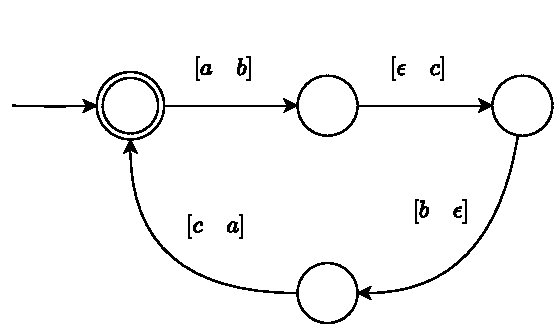
\includegraphics[scale=0.7,keepaspectratio]{jumps_synchronization-example_transducer_compact.pdf}
  \caption{
    Example of a 2-tape input/output \nft.
  }\label{fig:2_tape_nft}
\end{figure}

For example, the input word $abcabc$ is accepted on the input tape and produces a word $bcabca$ on the output tape.

\end{example}

\section{Data Structure}
\label{sec:mata_data_structure}
We propose utilizing the existing data structures in \mata (used for NFAs) for implementing finite transducers in \mata.
The main advantage is that NFAs, \nfts, and BDDs can all be implemented using the same single data structure, utilizing a lot of the existing algorithms on the data structures.

\mata provides a base class \nfaClass which encompasses both deterministic and non-deterministic finite automata and operations on them.
Class \nfaClass is a base class from which \nfts, BDDs, and register automata can inherit, including all operations on \nfaClass where only a few specific operations need to be modified for each respective type of finite state machines.
This hierarchy also allows us to add model-specific operations to each type of automata without modifying operations for the other automata.
BDDs in our representation only extend the functionality of \nfts, and can therefore inherit most of the algorithms from \nfts and only modify some of the algorithms for BDD-specific use-cases.

\begin{figure}[ht]
  \centering
  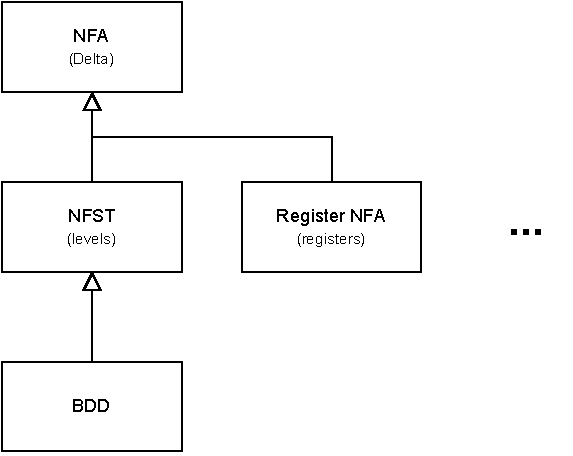
\includegraphics[scale=0.8, keepaspectratio]{jumps_synchronization-NFAs-NFSTs-BDDs-hierarchy.drawio.pdf}
  \caption{
    An inheritance hierarchy for NFAs, \nfts, BDDs, and register automata.
    All of these finite state machines utilize the same data structure, with mostly the same algorithms where only a few algorithms need to be modified for each respective type of finite state machines.
    Each type of finite state machines can further extend the set of operations by their own specific operations.
    Since BDDs only extend the functionality of transducers, BDDs can inherit directly from \nfts, modifying a few algorithms of \nfts together with the base \nfaClass algorithms.
  }
\end{figure}

Class \nfaClass defines which states in the represented automaton are initial (a set of initial states) and which are final (a set of final states).
Furthermore, \nfaClass allows for storing of arbitraty context in the automaton itself.

The most important data structure for the representation of the finite state machines and the efficiency of the algorithms run on the representation is the representation of transition relation, called \deltastruct in \mata.
\deltastruct defines the set of states of the finite automaton, and gives the transition relation of the finite automaton.
\deltastruct is designed in such a way that the often used operations such as iteration over transitions, or adding and removing transitions are performant, while the less used operations such as reversal of transition relation can be less performant.

States are represented as unsigned integers, numbered from 0.
This allows adding new states to the automaton to be as easy as getting the number of states in \deltastruct (constant time operation) and adding a number equal to the number of new states we want to add.
Such states are immediatelly allocated in \deltastruct and can be used in initial of final states sets.

Transition symbols are internally stored as unsigned integers as well, numbered from 0, where the last several unsigned integer values are reserved for epsilon symbols and special symbols (e.g., \emph{don't care} symbols in the proposed \nfts implementation).
\mata provides several alphabet types which map the actual transition symbols to their internal values.

The use of unsigned integers for states and symbols gives implicit ordering over both states and symbols and querying them by accessing index corresponding to the internal state/symbol value in an ordered vector.
\deltastruct is a three-level data structure where each level represents one element from the three-tuple $(q, s, q')$ representing a single transition as:
\begin{enumerate}
    \item source states,
    \item transition symbols,
    \item target states.
\end{enumerate}

Each level is internally stored in memory as a sorted vector of unsigned integers, stored in a low-level data structure provided by \mata called \ordvector, a wrapper over \texttt{std::vector} maintaining a set of elements inserted into \texttt{std::vector} ordered.

\ordvector therefore has constant time access to stored elements and operations on the largest element (implemented internally as \texttt{push\_back()}, \texttt{pop\_back()}), fast linear iteration over the elements, and linear union, intersection, and difference.
Since vectors are ordered, lookup for states and symbols is logarithmic using binary search.
Insertion and removal of elements are logarithmic, but they must shift elements in the memory in the underlying \texttt{std::vector} which slows the operations down.

Due to this, \mata tries to iterate over \ordvector as often as possible since internally, \texttt{std::vector} stores elements in a continuous array on heap with good memory locality, and add elements one after the other in an ascending order given by the value of the inserted elements at the end of the ordered vector.
\mata implements several algorithms for ease of use of the iteration such as synchronized traversal over multiple ordered vectors.
General insertion and removal of transitions are logarithmic, but \mata algorithms are written in such a way that the general insertion and removal are seldom used.

This pairs well with underlying data structures for sets of initial and final states, implemented as sparse sets~\cite{sparseset93} allowing for constant element lookup, insertion and removal, and fast linear iteration through elements.

The Figure~\ref{fig:delta_struct} visualizes the three-level \deltastruct data structure, as presented in~\cite{tacas24_mata_10.1007/978-3-031-57249-4_7}.
We can see that when we access by source state $q$ the index in the first vector of source states, we get a vector post of type \statepost (\statepost[q]), representing $\post(q)$, which is a vector of symbol posts for each transition symbol $a$ leading from source state $q$, of type \symbolpost.
Each symbol post for symbol $a$ represents $\post(q, a)$, storing the transition symbol $a$ and a set of target states represented as an \ordvector.

% {\tiny
\begin{figure}[ht]
  \centering
% TODO: Replace with my own image of Delta struct.
  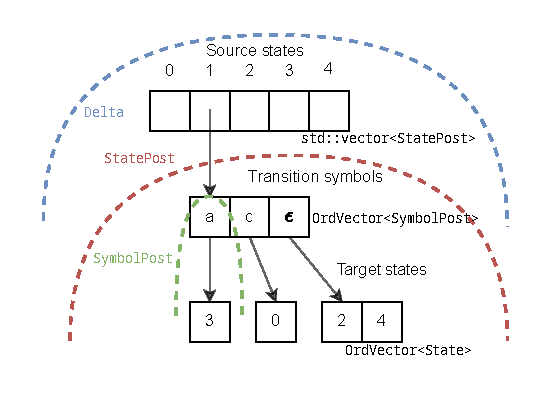
\includegraphics[keepaspectratio, scale=1]{subset_construction-delta.pdf}
  % \resizebox{0.6\textwidth}{!}{%
    % \definecolor{color1}{RGB}{54,174,124}
\definecolor{color2}{RGB}{24,116,152}
\begin{tikzpicture}[
    circ/.style={draw,circle,inner sep=0pt,minimum size=2pt,fill},
    arr/.style={->,thick,>=stealth},
    type/.style={color2,dashed,thick},
    % >=stealth,
]

\matrix[
    matrix of nodes,
    nodes={draw, minimum size=5mm},
    % column sep=-\pgflinewidth,
    row sep=0.5mm,
    nodes in empty cells,
    row 1/.style={nodes={draw=none, fill=none, minimum size=5mm}},
% row 1 column 1/.style={nodes={draw}}
] (delta) {
0 & 1 & 2 & 3 & 4 & 5 & 6 & 7 & 8 & 9\\
  &   &   &   &   &   &   &   &   &  \\
};
\node[below = 0cm of delta-2-8,xshift=4.5mm] {\code{std{::}vector{<}StatePost{>}}};
\draw[decoration={brace,amplitude=10pt}, decorate, color1, thick] (delta-1-1.north west) -- (delta-1-10.north east) node [above = 10pt, pos=0.5] {Source states};
\draw[type] plot [smooth,tension=2] coordinates {($(delta.west)+(-2,-5)$) ($(delta)+(0,1.5)$) ($(delta.east)+(2,-5)$)};
\node[right = 1cm of delta,color2] {\code{Delta}};

\matrix[
    matrix of nodes,
    nodes={draw, minimum size=5mm, anchor=center, %text centered, align=center
    },
    % column sep=-\pgflinewidth,
    % row sep=0.5mm,
    % nodes in empty cells,
    below = 1.3cm of delta-2-6
] (statepost) {
$a$ & $c$ & $e$ & $r$ & $x$ & $\epsilon$ \\
};
\draw[arr] ($(delta-2-5.north west)!0.5!(delta-2-5.south east)$) node[circ]{} .. controls +(0,-.7) and +(0,0.7) .. (statepost-1-1.north west);
\node[below = 0cm of statepost-1-5] {\ordvector{}\code{{<}SymbolPost{>}}};
\node[above = 0cm of statepost-1-4, color1] {Transition symbols};
\draw[type] plot [smooth,tension=2] coordinates {($(statepost.west)+(-1.5,-2.5)$) ($(statepost)+(0,1)$) ($(statepost.east)+(1.5,-2.5)$)};
\node[right = 0.8cm of statepost,color2] {\code{StatePost}};

\matrix[
    matrix of nodes,
    nodes={draw, minimum size=5mm, anchor=center, %text centered, align=center
    },
    % column sep=-\pgflinewidth,
    % row sep=0.5mm,
    % nodes in empty cells,
    below = 1.3cm of statepost-1-2
] (symbolpost1) {
1 & 3 & 5 & 6\\
};
\draw[arr] ($(statepost-1-2.north west)!0.5!(statepost-1-2.south east)+(0.17,0)$) node[circ]{} .. controls +(0,-.7) and +(0,0.7) .. (symbolpost1-1-1.north west);
\node[below = 0cm of symbolpost1-1-3] {\ordvector{}\code{{<}State{>}}};
\node[above = 0cm of symbolpost1-1-3, color1] {Target states};
\draw[type] plot [smooth, tension=1.1] coordinates {($(symbolpost1.south west)+(-0.2,0)$) ($(statepost-1-2)+(0,0.15)$) ($(symbolpost1.south east)+(0.2,0)$)};
\node[right = 0.2cm of symbolpost1,color2] {\code{SymbolPost}};

\end{tikzpicture}

  % }
% \vspace{-6mm}
\caption{
The vizualization of the three-level data structure representing the transition relation of a finite automaton in \mata, called \deltastruct.
}
\label{fig:delta_struct}
% \vspace{-4mm}
\end{figure}
% }

Notice that since \mata supports epsilon symbols as maximal unsigned integer values, the symbol posts for epsilons are always at the end of state posts and can be therefore accessed in constant time instead of having to search the whole state post to look them up. \mata operations utilize this fact in numerous operations using epsilon symbols such as in string solving~\cite{fm23_equations_synergy_regular_constraints_DBLP:conf/fm/BlahoudekCCHHLS23}.

\begin{example}
  Take a look at the example in Figure~\ref{fig:delta_struct_product_construction}.
  We perform an intersection of two \nfas (their transition relations at the top) using product construction, as described in Chapter~\ref{sec:Preliminaries}, constructing a product transition relation (at the bottom).
  \mata takes advantage of its $\deltastruct$ with ordered states and symbols.

  \begin{figure}
    %{r}{0.5\textwidth}
    [ht]
    \centering
  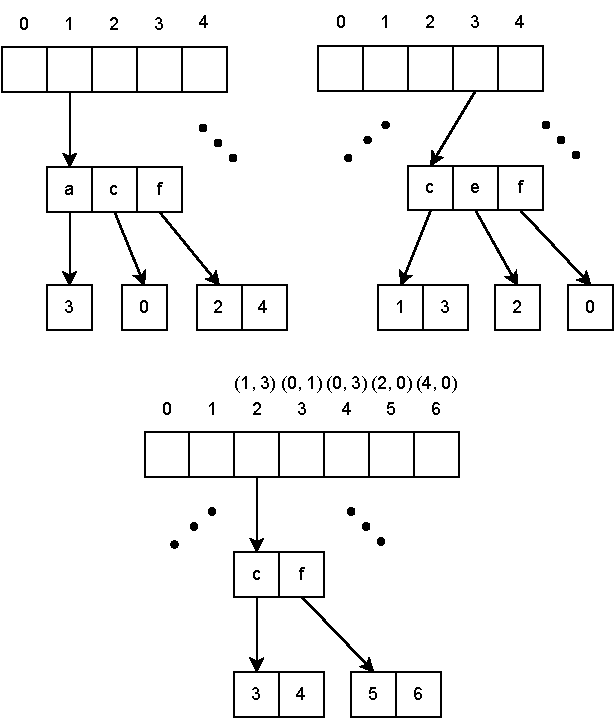
\includegraphics[keepaspectratio, scale=0.6]{subset_construction.drawio.pdf}
  \caption{
  The vizualization of intersection product construction on \nfas utilizing the advantages of the three-level transition relation \deltastruct.
  }
  \label{fig:delta_struct_product_construction}
  \end{figure}

  During the construction, new product transitions are often appended at the end of the existing vectors (algorithms try to minimize the number of binary searches in the lower levels in $\deltastruct$).
  In this example, computation of the new transitions for product state $(1, 3)$ creates $4$ new transitions, introducing new product states, e.g., $(0, 1)$ (product state $3$), and $(0, 3)$ (product state $4$).

  We can see that we first insert into a vector of target states for $\post(2, c)$ in the product product state $3$, and only then create a new product state $4$ and append it after the product state $3$.
\end{example}

\nfts and BDDs can directly utilize \nfaClass with all of the underlying data structures where one transition in \nft is represented by several transitions in \nfaClass.
The only modification of \nfaClass to support \nfts and BDDs is adding a vector of state \emph{levels} (represented by \texttt{std::vector}<unsigned>) indexed by automaton states, as in the first level in \deltastruct. The vector maps each automaton state to its level in the finite state machine.
$n$-tape \nft has $n$ levels.
Therefore, in a representation of an $n$-tape \nft, vector of state levels maps to values from $0$ to $n-1$.
One transition in \nft corresponds to $n$ transitions in \nfaClass.

Each transition in \nfaClass corresponds to one level of the \nft, i.e., one tape of the \nft.
\nft transition always starts at level $0$.
A transition from level $0$ to level $1$ represents the operation on the first \nft tape, from level $1$ to level $2$ the operation on the second \nft tape, and so on.
Finally, the transition from state with level $n-1$ back to state with level $0$ corresponds to the last tape in the \nft, finishing the sequence of \nfa transitions for a single \nft transition.

For 2-tape (input/output) \nft, the levels used will be $0$ and $1$, where transitions from states with levels $0$ represent the input transitions and transitions from states with levels $1$ represent the output transitions.

We denote a level $l$ of a state $q$ as $l = \level{q}$.
Since levels directly represent their corresponding tapes, we use terms \emph{level} and \emph{tape} interchangeably when the meaning is clear.

For this reason, \nfts can have only states $q$ with $\level{q} = 0$ as initial or final states.
This is crutial for many algorithms (more in~\ref{sec:Algorithms}) which rely on certain invariants in the representation of \nfts, such as that \nfts always synchronize in states with state level $0$ and each step in operations must consider the entire state levels sequence from $0$ to $n-1$ as a single \emph{abstract} step (a single complete \nft transition).

\subsection{Epsilon and Don't Care Transitions}

\nfts and BDDs also need suport for epsilon symbols and don't care symbols on transitions.

\mata already supports epsilon symbols as (several) last transition symbol(s) in the range of possible transition symbols given by the data type of transition symbol.
Adding support for \emph{don't care} symbols on transitions, matching any transition symbol on the tape, is similar to epsilon symbols.

An epsilon symbol on a transition from state with level $k$ to level $k + 1 \text{ mod } n$ in \nfaClass representing an \nft means that the tape corresponding to the level $k$ does not read from~/~write on the tape $k$ any symbol.

\nfts, but mainly BDDs represented as \nfaClass also require support for \emph{jumps} where the transition goes from a state with level $k$ to any other state with level $l$ where $l \neq k + 1$.
However, we restrict the jumps for $n$-tape \nft as follows:
\begin{itemize}
  \item The jump cannot jump over a state with level $0$.
  That is, if we need to jump further, the transition can at most jump to the next state with level $0$.
  \item A jump of length $k > 1$ (the length of one is a normal transition in \nfaClass which we call just a transition) is interpreted the same as if we made $k$ transitions in \nfaClass with the transition symbol on the jump transition.
  That is, a jump of length $3$ (over $3$ tapes) with transition symbol $\epsilon$ means that the transducer made $3$ normal transitions with $\epsilon$ as a transition symbol for each of them.
  \item Jumping from a state $q$ where $\level{q} = 0$ to a next state $q'$ where $\level{q'} = 0$ with transition symbol $\epsilon$ means that only the internal state of the \nft has changed (the state has changed) without reading or writing anything on any of the tapes.
  \item Jumping from a state $q$ where $\level{q} = 0$ to a next state $q'$ where $\level{q'} = 0$ with transition symbol $a \in \Sigma$ means that we performed an identity \nft transition over $a$ where all tapes read/write symbol $a$.
\end{itemize}

% TODO: Figure for jumps.




\begin{example}\label{example:2_tape_nft_in_mata}
  The \nft from Example~\ref{example:2_tape_nft} is represented in the data structure for \nfts inherited from \nfaClass as in the Figure~\ref{fig:2_tape_nft_in_mata}.

  Transitions from states with level $0$ represent the input tape, and transitions from states with level $1$ represent the output tape.

  \begin{figure}[ht]
    \centering
    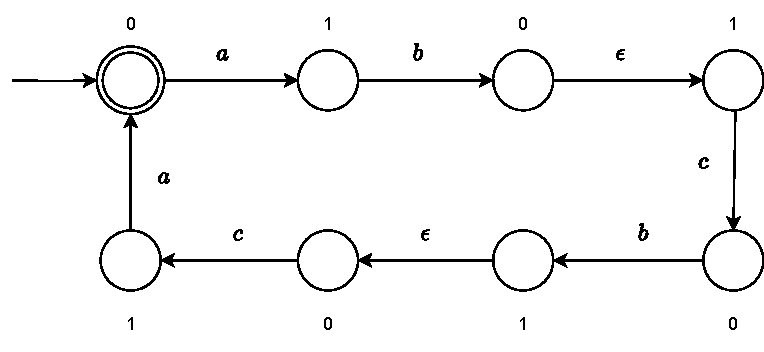
\includegraphics[scale=0.7,keepaspectratio]{jumps_synchronization-example_transducer_mata.pdf}
    \caption{
      $2$-tape \nft from Example~\ref{example:2_tape_nft} represented in \mata as an \nfaClass with states annotated by levels.
    }\label{fig:2_tape_nft_in_mata}
  \end{figure}

Intuitively, we can still see that the same rewriting rules apply.
The input word $abcabc$ is still accepted on the input tape and produces the same word $bcabca$ on the output tape.

\end{example}

\subsection{No Operation Transitions}
An epsilon transition from a state with level $k$ to $k+1 \mod n$ can be understood as a \emph{no operation transition} \nop, i.e., a transition where the current tape does not perform any operation (no reading nor writing). In essence the impact of the transition is the same as if reading an empty string on the current tape.

In constrast, an epsilon transition from a state with level $k$ to another state with level $k$ is a simple change of states (as per the usual definition of epsilon transitions in \nfas).

Depending on the application, one might prefer to use one or the other representation as needed.
In this work, we use \nop when we want to explicitly stress the distinction between a simple change of state in \nft (an epsilon transition between states with the same level), and no operation on a current tape (the tape does not read nor writes any symbol).

\section{Algorithms}
\label{sec:Algorithms}

For general uses of transducers in \mata, we have implemented general automata operations for creating, modifying, and manipulating transducers.
Furthermore, we have implemented several transducer-specific operations.

\paragraph{\nfa operations.}
The general \nfa operations such as concatenation, union, etc. can be reused from \nfa without many modifications.
We only need to remember to correctly set levels of states when renumbering states in the result \nft.

Further, we discuss several more significant modifications to existing operations and algorithms for several \nft-specific operations.

\subsection{Synchronization}

All operations performing some kind of traversal over multiple transition relations (or multiple transitions in one transition relation simultaneously) start the compution from states with level $0$.
\nfts are always synchronized on states with level $0$, that is, after each \nft transition is completed (all tape operations are handled).
If the macrostate in a worklist contains only states with levels $0$, the \nfts are synchronized and the next macrostate can be computed.
When the synchronized \nfts perform one transition, due to the supported jumps, the new macrostate may contain states with different levels.
Only the state in the macrostate with the level furthest behind is expanded (performs its transitions, if possible).
The others are at least one level ahead and therefore cannot be expanded and must wait for the states behind to get to at least their levels first before being expanded themselves.

Since jumps can jump at most to the next state with level $0$, we always know which states in the macrostate are ahead and which are behind by the following method.
If we expand a macrostate with states with levels $k$ and $l$ where $k > l$, we know that state with level $k$ must be ahead of the state with level $l$.
If any of the states has level $0$ (and there are other states with nonzero levels), we know that the state $0$ must be ahead of all the other states with nonzero levels, and synchronized with all other states with levels $0$.
That holds since the states with levels $0$ can only be the next states with levels $0$, and not the states with level $0$ behind (as the first step from the synchronized states is to move immediately out of the states with level $0$).

The same holds for BDDs utilizing the same data structure and constraints as \nfts.

\begin{example}
  If we perform synchronization over three $4$-tape \nfts, starting from macrostate with levels $(0, 0, 0)$, we perform one transition and may end up in a macrostate with levels $(3, 1, 0)$ where the first \nft made a jump of length $3$, the second performed normal transition (jump of length $0$), and the last \nft performed a jump to the next state with level $0$.
  When expanding the macrostate $(3, 1, 0)$ later on, we know that the state with level $0$ is ahead of the other states with levels $3$ and $1$. And we further know that state with level $3$ must be ahead of the state with level $1$. Therefore, the state with level $1$ must be expanded up until the level reaches $3$ or greater (the next level $0$).
  Then we may get $(3, 3, 0)$, both the first and the second state are expanded to states with levels $(0, 0, 0)$ and the macrostate is synchronized again.

  The Figure~\ref{fig:synchronization_jumps} shows an example of how may synchronization on a pair of \nfts using jumps look.
\end{example}

\begin{figure}[ht]
  \centering
  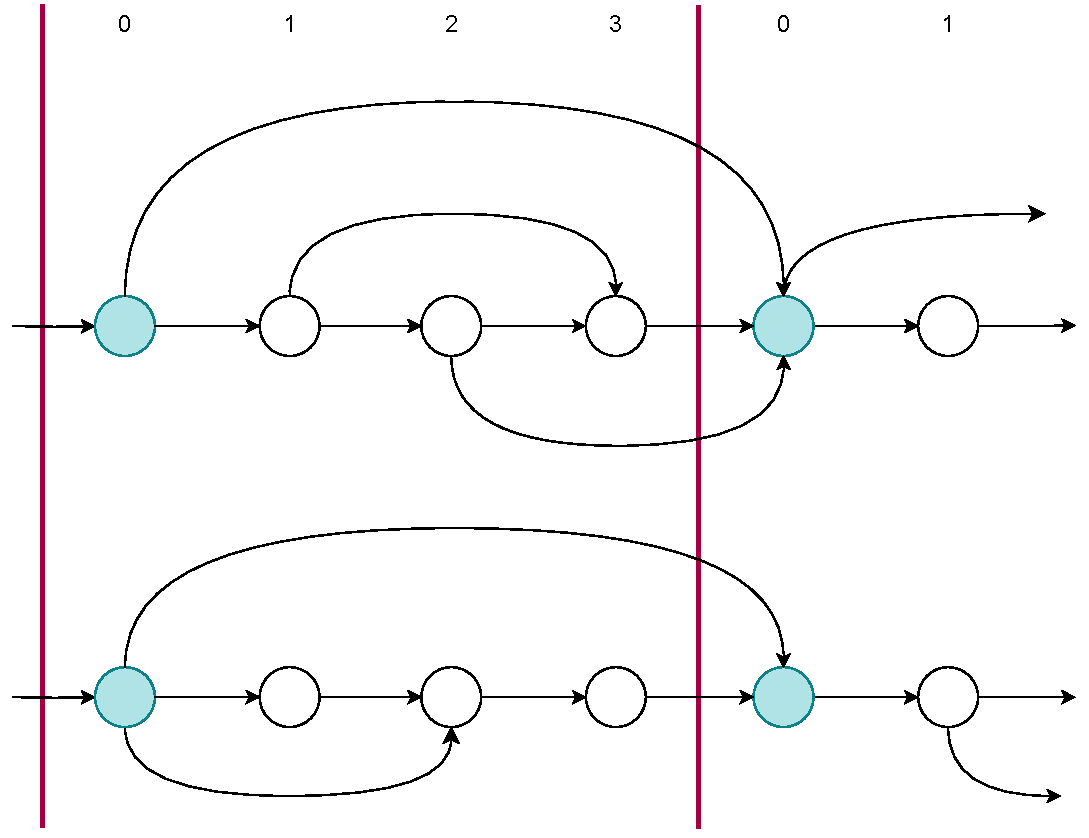
\includegraphics[scale=0.5, keepaspectratio]{obrazky-figures/jumps_synchronization.drawio.pdf}
  \caption{
    An example of $4$-tape \nfts with jumps during synchronization.
    Jumps can start in state with any level and jump up to the next state with level $0$.
    The jumps cannot jump over states with level $0$, however.
    The numbers denote the levels for the corresponding states below.
    The highlighted states depict the states with level $0$, the vertical lines visually set apart \nft transitions (there is one \nft transition, consisting of several tapes, between each pair of vertical lines).
  }
  \label{fig:synchronization_jumps}

\end{figure}

\paragraph{Alternative representation of jumps.}
If the restriction of allowed jumps being only to the next state with level $0$ is too strict, an alternative approach where jumps are allowed to jump over (potentially multiple) states with level $0$ can be chosen.
However, during operations such as product construction, an additional information must be added to the worklist containing macrostates containing a list of lengths of each jump performed during the expansion of the last macrostate in order to know how far ahead are the states jumped to in relation to the other states in the macrostate.

We deem this approach inferior to our chosen approach since it distorts the simplicity of a single data structure and algorithms on it for NFAs, \nfts, and BDDs.

% ==================================
\subsection{Projection}\label{sec:projection}

The first standard operation on transducers is \emph{projection}.
Given an $n$-tape \nft $\ft$, we can perform \emph{projection to} a specified set of tapes, or \emph{project out} a specified set of tapes.

The transitions remain the same, the only change is that we remove certain tapes (meaning that for every \nft transition we remove transition symbols on those tapes).
In \mata, this means removing all states with certain levels $k$ and their outgoing transitions and redirecting ingoing transitions to these states to the next states with levels $k + 1 \mod n$ where the outgoing transitions were previously leading to.
This can be iteratively performed on all tapes specified for removal.
When the modification is performed, all remaining levels are shifted toward $0$ to start at $0$ and end with $l - 1$ where $l$ is the new number of tapes remaining in the \nft.

Projection to, denoted $\projToSet{M}{\ft}$ where $M \subseteq \{ 0, 1, \ldots, n - 1 \} $ is an operation which keeps only tapes $t \in M$, and removes from $\ft$ all other tapes $o \notin M$.
In practice, this means that an $n$-tape \nft will be modified into an $|M|$-tape \nft.
If $|M| = 1$, we create a $1$-tape \nft (containing only states with level $0$) which is semantically equivalent to a corresponding \nfa with the same transitions.

Projection out, denoted $\projOutSet{M}{\ft}$, performs the same operation, only now instead of keeping the specified tapes $o \in M$, we remove all tapes $o \in M$, and keep only the tapes $t \in \{ 0, 1, \ldots, n - 1 \} \setminus M$.
If $|M| + 1 = n$, we project out all tapes except for one.
This creates a $1$-tape \nft, which is again semantically equivalent to a corresponding \nfa with the same transitions.

Note that for either variation, removing the first tape in \nft transitions requires setting new initial states (the original targets of transitions from the states with level $0$ become the new initial states).
Similarly, removing the last tape in \nft transitions requires setting new final states (the original source of ingoing transitions to the final states become the new final states).
If jump transitions are involved, one may need to expand the jumps into normal transitions between levels to set the correct initial and final states on the new first and last tape.

\begin{example}
  Given an \nft $\ft$ with $5$ tapes, with levels $\{ 0, 1, 2, 3, 4 \}$.

  We can perform the following operations:
  \begin{itemize}
    \item $\projOutSet{\{ 3 \}}{\ft}$ which deletes tape $3$ from $\ft$, leaving tapes $\{ 0, 1, 2, 4 \}$ which are then renumbered to $\{ 0, 1, 2, 3 \}$.
    \item On the result, we can perform $\projToSet{\{ 1, 3 \}}{\ft}$ which performs the same as if calling $\projOutSet{\{ 0, 2 \} }{\ft}$.
    Tapes $0$ and $2$ are removed, leaving tapes $\{ 1, 3 \}$, which are then renumbered to $\{ 0, 1 \}$.
    \item Now, peforming $\projToSet{\{ 1 \}}{\ft}$ gives us \nft with only one tape, which represents the \nfa for the tape $1$.
    Performing $\projOutSet{\{ 1 \}}{\ft}$ instead would give us \nft with only one tape representing the \nfa for the tape $0$.
  \end{itemize}

\end{example}

% ==================================
\subsection{Intersection}\label{sec:intersection}

For constructing the intersection of two \nfts, we make use of the inheritance of \nfts from \nfas and utilize the classic intersection computation on \nfa using the standard product construction algorithm (as described in Chapter~\ref{sec:Preliminaries}).
The only modification is adding support for proper assignment of levels to new macrostates depending on the levels of the original \nft states in the macrostate, and handling of various combinations of transition symbols during the process of adding transitions leading from the macrostates.

Given $\ft_1$ with $\states_1$ and $\ft_2$ with $\states_2$, construct the intersection $\ft = \ft_1 \cap \ft_2$.

A new level $\level{q'}$ for a new macrostate $q' = (q'_1, q'_2)$, given a current macrostate $q = (q_1, q_2) \in \states_1 \times \states_2$ where $q'_1$ and $q'_2$ are targets of transitions from $q_1$ and $q_2$, is determined as follows:
\begin{itemize}
  \item If $\level{q'_1} = 0$ or $\level{q'_2} = 0$ (holds for both equal $0$, too), $\level{q'} = \texttt{max}(\level{q'_1}, \level{q'_2})$. If both target states have levels $0$, we are finishing an entire \nft transition and enter a synchronized macrostate $q'$, $\level{q'} = 0$. Otherwise, only $q'_1 = 0$ ($q'_2 = 0$) holds, and $q'_1$ ($q'_2$) must be ''further ahead'' of $q'_2$ ($q'_1$), and must wait for $q'_2$ ($q'_1$) to catch up, therefore, $0 < \level{q'} < n$.
  \item Otherwise, $\level{q'} = \texttt{min}(\level{q'_1}, \level{q'_2})$. That is, if both $0 < \level{q'_1}, \level{q'_2} < n$, we must wait for the state further behind to catch up, so we choose the lower level as $\level{q'}$.
\end{itemize}

A new transition symbol $a \in \Sigma$ for a new transition $(q, a, q')$ is chosen by the following rules:
\begin{itemize}
  \item If $(q_1, a, q'_1) \in \post_1$ and $(q_2, a, q'_2) \in \post_2$, $(q, a, q') \in \post$.
  \item If $(q_1, \epsilon, q'_1) \in \post_1$ and $(q_2, \epsilon, q'_2) \in \post_2$, $(q, \epsilon, q') \in \post$. Epsilon symbols are handled here as normal symbols $a \in \Sigma$. This ensures that only matching $\epsilon$ symbols are synchronized.
  \item If $(q_1, \dontCare, q'_1) \in \post_1$ (or $(q_2, \dontCare, q'_2) \in \post_2$), $a$ from $(q_2, a, q'_2)$ ($(q_1, a, q'_1)$) is used.
  This holds for $(q_1, \dontCare, q'_1) \in \post_1$ and $(q_2, \dontCare, q'_2) \in \post_2$, too.
  This works if one of the symbols is $\dontCare$ and the other is $\epsilon$, too: $(q, \epsilon, q')$ is produced in such a case.
\end{itemize}

The rules are visualizated in the Table~\ref{tab:synchronization_rules}.
\begin{table}[ht]
\centering
\begin{tabular}{ |c||c|c|c|c| }
 \hline
 $\cap$ & $\dontCare$ & $\epsilon$ & a & b \\
 \hline
 \hline
 $\dontCare$ & $\dontCare$ & $\epsilon$ & a & b \\
 \hline
 $\epsilon$ & $\epsilon$ & $\epsilon$ & & \\
 \hline
 a & a &  & a &\\
 \hline
 b & b &  & & b\\
 \hline
\end{tabular}
\caption{
  Synchronization rules for transitions symbols during intersection.
  The row lists the symbols on transitions in $\ft_1$, the column in $\ft_2$.
}
\label{tab:synchronization_rules}
\end{table}

Finally, $\dontCare$ transitions must be handled separately since the classic intersection algorithm for \nfas does not match $\dontCare$ with any other symbol than $\dontCare$.

% ==================================
\subsection{Composition}

When working with \nfts as transduction machines taking some input, modifying it and outputting some output, we often encounter problems where we want to perform multiple transductions on the input, one after the other.
In the same way as we can compose mathematical functions $(f \circ g)(x)$ meaning $f(g(x))$ (perform $g$ on $x$ and perform $f$ on the result of $g(x)$),
we can perform multiple \nft transductions sequentially: $\ft_2 \circ \ft_1$
(perform the transduction of $\ft_1$ on the input, and then perform the transduction of $\ft_2$ on the result), denoted as $\compose{\ft_1}{\ft_2}$.
Using the Unix \emph{pipe} notation, we can express the same with $\ft_1 \composePipe \ft_2$
(perform the transduction of $\ft_1$ on the input, and then pipe the result to $\ft_2$ to perform the transduction of $\ft_2$ on the result).

For each \nft, we need to specify which tape(s) $T$ to synchronize on with the other \nft.
These are the tapes we expect to act as a mediator between the output of $\ft_1$ and the input of $\ft_2$.
To create a new product transition, the symbols on the corresponding tapes in both \nfts must be compatible (the same symbol, or pairs like $(\dontCare, a)$ for $a \in \Sigma$, etc.).
% TODO: Explain synchronization better.

The composition comprises the following steps:
\begin{itemize}
  \item Extending the \nfts to contain matching tapes,
  \item Adding special self-loops on states with level $0$ to allow for proper handling of $\epsilon$ and $\dontCare$ symbols on the transitions,
  \item Performing \nft intersection as described in Section~\ref{sec:intersection}, and
  \item Projecting out the synchronization tapes (as described in Section~\ref{sec:projection}) which were ''consumed'' by the composition.
\end{itemize}

\begin{example}
  Throughout this section, we will demonstrate the composition algorithm on the following example.
  Given \nft $\ft_1$ with tapes $0$, $1$, and $2$, and $\ft_2$ with tapes $2$, $3$, and $4$, we want to compute $\ft_1 \composePipe \ft_2$, synchronizing both \nfts on tape $2$.
  For clarity, we number the tapes uniquely between both \nfts in this example. Internally, each \nft has tapes with levels from $0$ to $2$ and for each \nft, we specify which tape(s) the \nfts should synchronize on.
\end{example}

\paragraph{Extending \nfts to match each other.}
The first step of the composition is to extend the input \nfts by inserting additional levels $k$ (additional states with levels $k$) into each transition with $\dontCare$ symbols on the transitions at levels $k$.
This operation balances out the \nfts so both have the same tapes in the same order.
This allows us to perform the classic \nfa intersection for each level in both \nfts during \nft intersection.
We use $\dontCare$ symbols since for each \nft $\ft_i$, the other \nft $\ft_j$ does not care what transitions over what symbols $\ft_i$ performs during the intersection.
Hence, from the point of view $\ft_j$, $\ft_i$ can perform any transition.

\begin{example}
  Continuing the example, we extend each \nft transition in $\ft_1$ with new transitions as follows: from existing states $q_2$ with level $2$ to new states $q_3$ with levels $3$ (using the original transition symbol on transitions outgoing from $q_2$), from $q_3$ to new states $q_4$ with levels $4$ using $\dontCare$ symbol, and finally from $q_4$ to the next existing states $q_0$ with levels $0$ (the orinal targets of transitions from $q_2$) using $\dontCare$ symbol (finishing the original \nft transition).

  Figure~\ref{fig:composition_nfts_extension} shows a depiction of a single transition in $\ft_1$ and $\ft_2$ before and after extension.

  \begin{figure}[ht]
    \centering
    \subfloat[\centering Before extension\label{fig:composition_nfts_extension_before}]{{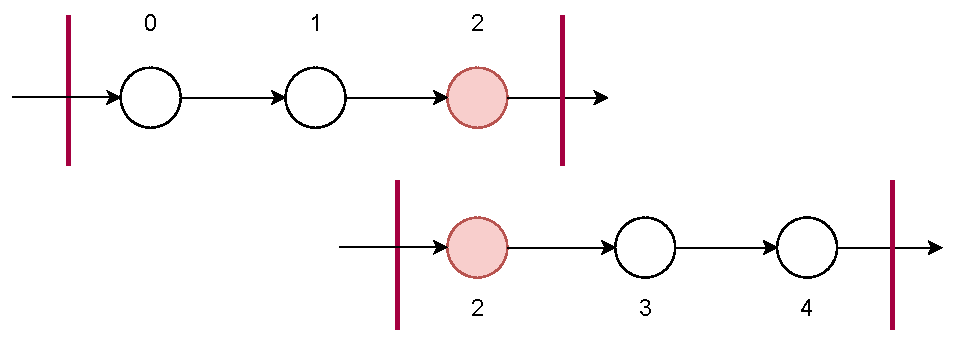
\includegraphics[keepaspectratio,width=0.45\textwidth]{jumps_synchronization-composition_nfts_extension.pdf} }}%
    \qquad
    \subfloat[\centering After extention\label{fig:composition_nfts_extension_after}]{{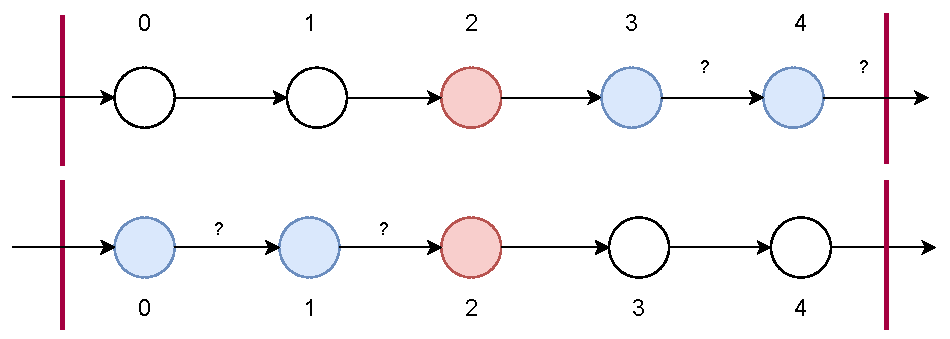
\includegraphics[keepaspectratio,width=0.45\textwidth]{jumps_synchronization-composition_nfts_extension_balanced.pdf} }}%
    \caption{
      A depiction of a single transition in \nfts $\ft_1$ (top) and $\ft_2$ (bottom) before extension (Figure~\ref{fig:composition_nfts_extension_before}) and after extension with $\dontCare$ transitions on inserted tapes to balance out the tapes in both \nfts (Figure~\ref{fig:composition_nfts_extension_after}).
      The red states together with the outgoing transitions represent the tape $\ft_1$ and $\ft_2$ are synchornized on.
      The blue states represent the newly inserted tapes with $\dontCare$ symbols on transitions.
    }
    \label{fig:composition_nfts_extension}%
  \end{figure}

  We can see that after the extension, both $\ft_1$ and $\ft_2$ have the same tapes.
\end{example}

Thanks to this general approach, we can compute compositions of any $n$-tape and $m$-tape \nfts, synchronizing on any tape(s)\footnote{When synchronizing on multiple tapes, the tapes must be in the same order in both \nfts.}, with the tapes being in an arbitrary order.

As an optimization, when adding multiple subsequent $\dontCare$ transitions during the extension, we can instead add only a single $\dontCare$ jump from the first state in the sequence leading to the last state in the sequence, without having to create new states for all inserted tapes being jumped over.

\paragraph{Adding self-loops.}
The next step is to add self-loops to all states with level $0$ in both \nfts.
These self-loops serve the purpose of nondeterministic ''waiting'' loops for waiting at the beginning of an \nft transition in one \nft for the other \nft for epsilon transitions on the tapes being synchronized on.

The self-loops is a symbolic name since they are self-loops in the sense of \nft transitions (from state with level $0$ back to the same state), but they lead over several tapes (i.e., several states with transitions).

The symbols on the self-loops are added as follows:
\begin{itemize}
  \item For the transitions on the synchronization tapes, the symbol $\epsilon$ is used, being handled as a normal transition symbol the other \nft can synchronize with the $\epsilon$ symbol on any non-self-loop transition.
  \item For the transitions on tapes added by the extension, the symbol $\dontCare$ is used.
  $\dontCare$ here has the same role as $\dontCare$ symbols added during extension.
  \item For the transitions on the remaining tapes (the original non-synchronizing tapes), $\epsilon$ symbol is used to represent the waiting on all \nft's own transitions.
\end{itemize}

\begin{example}
  Figure~\ref{fig:composition_nfts_extension_loops} shows how a single transition in \nfts looks after adding the ''waiting'' self-loops.
  \begin{figure}[ht]
    \centering
    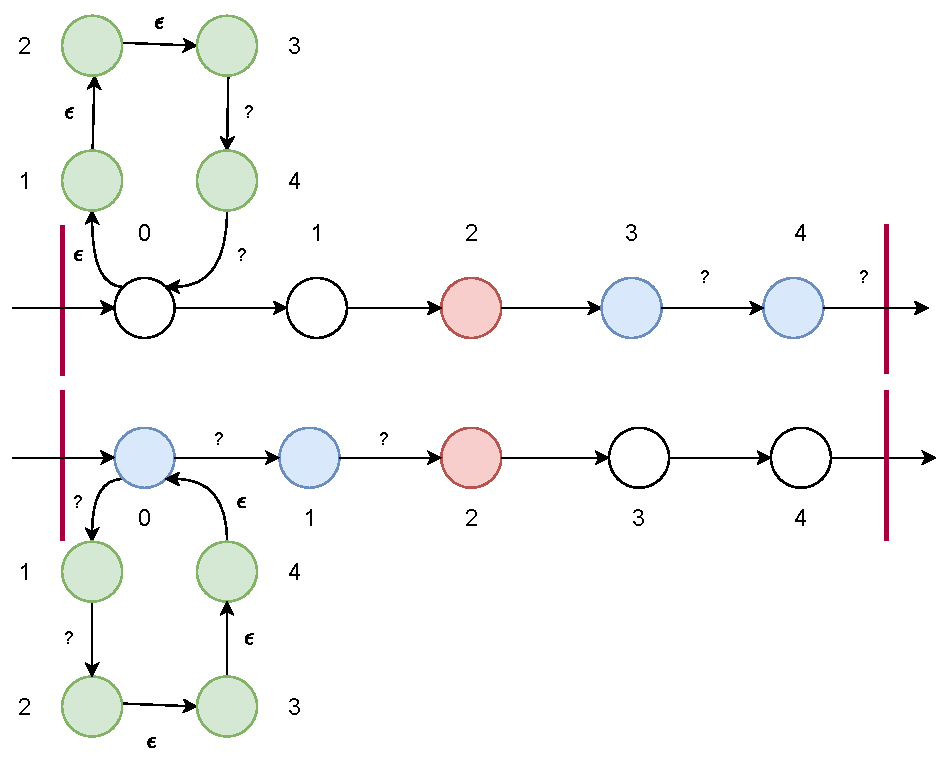
\includegraphics[keepaspectratio, width=0.5\textwidth]{jumps_synchronization-composition_nfts_extension_loops.pdf}
    \caption{
      A depiction of a single transition in \nfts $\ft_1$ (top) and $\ft_2$ (bottom) after adding the ''waiting'' self-loops.
    }
    \label{fig:composition_nfts_extension_loops}
  \end{figure}
\end{example}

\paragraph{Intersection.}
When the \nfts are balanced out and self-loops are added, we can perform an \nft intersection, as per Section~\ref{sec:intersection}.
The intersection produces a new \nft representing the composition of $\ft = \ft_1 \composePipe \ft2$, only currently $\ft$ still contains all the tapes from the balanced $\ft_1$ and $\ft_2$.
Other that that, the composition is complete.

Note that since we added the self-loops, we no longer need to separately handle $\epsilon$ transitions.
$\epsilon$ symbols are handled as normal transitions, producing an $\epsilon$ transition in the product iff both \nfts perform an $\epsilon$ transition, or one of them performs a $\dontCare$ transition.

Furthermore, we prevent self-loops in both \nfts from synchronizing with each other.
 That is, we cannot construct a new macrostate $q' = (q_{l1}, q_{l2})$ where both $q_{l1}$ and $q_{l2}$ are self-loop states.
This would represent a situation where both \nfts are waiting for the other, but none moves forward.
Since these macrostates are not useful, we prevent their creation entirely.

\paragraph{Projecting out the tapes the composition synchronized on.}
To clean up $\ft$, we need to project out the tapes we synchronized on as these are the tapes that have been ''consumed'' by the composition (used as the link between the output of $\ft_1$ and input of $\ft_2$).

\begin{example}
  To finish out example, Figure~\ref{fig:composition_nfts_extension_final} depicts a single product transition after composition is performed and the synchronization tapes are projected out.
  \begin{figure}[ht]
    \centering
    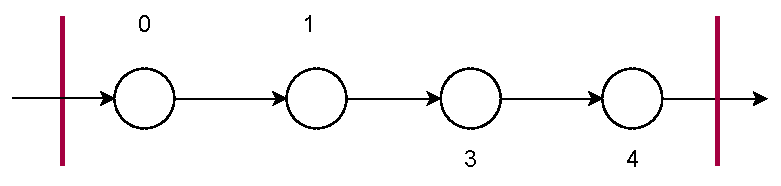
\includegraphics[keepaspectratio, width=0.5\textwidth]{jumps_synchronization-composition_nfts_extension_final.pdf}
    \caption{
      A depiction of a single product transition in $\ft = \ft_1 \composePipe \ft_2$ synchonized on tape $2$.
      The levels at the top represent the original tapes before renumbering.
      The levels at the bottom represented the final tapes after renumbering.
    }
    \label{fig:composition_nfts_extension_final}
  \end{figure}
\end{example}

\paragraph{Optimization for $2$-tape \nfts.}
For working with only $2$-tape \nfts, a specialized algorithm for composition can be utilized.
We presume that input/output \nfts always input on the first tape and output on the second tape.
The algorithm would still utilize the general idea of \nft intersection, but now no extension of \nfts and no self-loops are necessary.
For each macrostate, we would first perform a step in $\ft_1$ on level $0$, then perform the synchronized step on levels $1$ in $\ft_1$ and $0$ in $\ft_2$ (if such a step is possible as per \nft intersection rules), then finish the composition of the current transition by performing a step in $\ft_2$ on level $1$, constructing a new macrostate from targets of transitions on levels $1$ of both \nfts.
Handling of jumps is similar to \nft intersection: waiting for the state ''left behind'' to catch up with the state jumped to.
This approach no longer handles $\epsilon$ symbols as normal symbols $a \in \Sigma$, but instead uses the classic synchronization on $\epsilon$ symbols used in the intersection for \nfas.

When adding support for transducers to \noodler, it may be advantageous to utilize this specialized variation of composition as string replace operations in \noodler only ever work with $2$ tapes.

% ==================================
\subsection{Application}

When we construct an \nft $\ft$, the most intuitive use of $\ft$ is to perform the transduction $\ft$ encodes (reading the input on the input tapes and outputting the output on the output tapes) .
This operation is called \emph{application}.

We can \emph{apply} a word $w$ on $\ft$, or a regular language $\langof{\aut}$ for some $\aut$.

\paragraph{Application of a word.}
We can either apply a word $w \in \Sigma^*$ on a given tape (at level $k$), or apply an $l$-tuple of words $(w_i)$ where $l < n$, $i \in \{ 0, \ldots, n - 1 \}$ and $i$ specifies on which tape (level) we want to apply the respective words (one word $w_i$ for tape $i$).

The result of the application of a word (or a tuple of words) is a set of tuples of size $(n - l)$ of words.
We read the word(s) being applied and move through the \nft according to the transition symbols in the applied word(s) on the corresponding tapes, similarly to performing a run on a word in \nfa, only now to potentially multiple tapes (multiple words).
During the traversal, we construct the result by appending the transition symbols on the remaining tapes to the result constructed so far for the current state.
This gives us the corresponding word on the remaing tapes when the words on the given tapes are $(w_i)$.

Focusing on $2$-tape \nfts $\ft$, the application equals to translation from the input word $w$ to the output word $w'$ (similarly to what a natural language translator does) where $w' = \apply{\ft}{w}$.
By convention, we presume the input tape is at level $0$ and the output tape is at level $1$.

The application of a word is equivalent to $\idNft{\aut} \composePipe \ft$ where $\aut$ represents a \dfa accepting only $w$.
This gives us an \nft encoding the result.
For $2$-tape $\ft$, we get a $1$-tape \nft, equal to the corresponding \nfa encoding the set of words in the result.

\paragraph{Application of a language.}
Applying a regular language $\langof{\aut}$ on $n$-tape \nft $\ft$ instead of a single word is performed similarly to the application of a single word, but now the result is a regular language (for $2$-tape \nfts) or an \nft $\ft'$ with $n-1$ tapes.

The application of a language $\langof{\aut}$, similarly to the application of a word, is equivalent to $\idNft{\aut} \composePipe \ft$.
The resulting \nft encodes the result.
For $2$-tape $\ft$, we get a $1$-tape \nft, equal to the corresponding \nfa encoding the regular language of the result.

\chapter{Transducers for String Solving}

We discuss in this chapter how to utilize finite transducers in \noodler to solve SMT string constraints \texttt{str.replace}, \texttt{str.replace\_re}, \texttt{str.replace\_all} and\\\texttt{str.replace\_re\_all}.

\section{Replace Operations}
A general regular replacement operation has the following form:
\begin{center}
\begin{verbatim}
  replaced_string = replace(input_string, pattern, replacement)
\end{verbatim}
\end{center}
where \texttt{replace} determines the type of the regular replacement (the semantics of the replacement operation).
\texttt{input\_string} represents the original input string where we want to replace some regular \texttt{pattern} with a \texttt{replacement} literal.
Regular \texttt{pattern} can be a string literal (a word) or a regular language describing the substring (or substrings) of \texttt{input\_string} we are trying to replace.

There are various replacement semantics for replace operations. The popular regular replacement types are \emph{reluctant replacement}, \emph{greedy replacement}, \emph{possessive replacement}, or \emph{declarative replacement}.
For example, the reluctant replacement matches a given \texttt{pattern} (a regular language) with the shortest substring of the \texttt{input\_string}, while the greedy replacement matches the longest substring. These types produce the same result when \texttt{pattern} is a string literal.
Possessive replacement semantics is that of the greedy one, but without backtracking on the substring matched so far (we match on the first longest match).
Declarative replacement matches every occurrence of regular \texttt{pattern} in the given \texttt{input\_string}.

A \emph{procedural} regular replacements enforce the matching of the left-most occurrence of \texttt{pattern}.
Procedural replacements encompass the greedy and reluctant replacements since both match in \texttt{input\_string} from the left to the right.
They start with the first character in the word and by using backtracking continue through the word until the end of the word.

Since SMT-LIB defines only replacement operations of type reluctant replacement with the left-most matching and other types of the replacement operations are not allowed in SMT formulae in SMT-LIB format (which \noodler solves), we focus in this work solely on the reluctant replacement type.

We denote reluctant regular replacement as $x_{\pi \rightarrow y}$ where $x$ is the \texttt{input\_string}, $\pi$ is the regular \texttt{pattern} (a literal or a regular language) and $y$ is the \texttt{replacement}.

\section{Encoding Reluctant Replacement as Transducers}

SMT-LIB suports two types of reluctant replacements: a \emph{reluctant all replacement} which replaces all occurrences of the shortest left-most matches of \texttt{pattern}, and \emph{reluctant single replacement} which replaces only the first shortest left-most occurrence of \texttt{pattern}.

\paragraph{Empty word in \texttt{pattern}.}
If the \texttt{pattern} contains an empty word $\epsilon$, a special handling of $\epsilon$ matching needs to be performed. In such a case, one encodes the replacement operation as if $\epsilon \notin \pi$, and solves the replacement for two options:
\begin{itemize}
  \item Tries solving for just $\epsilon$ manually, and alternatively
  \item Solves the reluctant replacement without the epsilon if the $\epsilon$ match fails.
\end{itemize}
Since SMT-LIB works only with reluctant replacements, the reluctant replacement would always pick the shortest replacement, i.e., the $\epsilon$ replacement. The reluctant match of $\epsilon$ will always succeed and longer matches will not be needed nor accepted. SMT-LIB declares results to such patterns with $\epsilon$ to be equal to $\texttt{replacement} \concat \texttt{input\_string}$ (prepending the replacement to the \texttt{input\_string}).
No replacement \nft needs to be constructed in this case.

% Define reluctant replacement.

\begin{definition}[\textbf{Reluctant all replacement}] \hfill \newline
  A \emph{reluctant all replacement} $x^{+}_{\pi \rightarrow y}$ is defined as follows: \newline
  $$x^{+}_{\pi \rightarrow y} = \{ u \concat y \concat w^{+}_{\pi \rightarrow y} \}$$
  where $u, v, w, x, y \in \Sigma^*$, $\pi$ is a regular language (regex), $x = u v w$, $u \notin \Sigma^* \pi \Sigma^*$, $v \in \pi$, and to ensure the shortest left-most matching, the following must hold: $\forall u = u_1 u_2, v = v_1 v_2, w = w_1 w_2:$ if $v_2 \neq \epsilon$ then $v_1 \notin \pi$ (the shortest match---if $v_1$ is not a match, then surely the shortest match is $v = v_1v_2$);
  if $u_2 \neq \epsilon$ then $u_2 v_1 \notin \pi \land u_2 v w_1 \notin \pi$ (the left-most match is $v$ since there is no match of $\pi$ before $v$).
\end{definition}

A reluctant single replacement is defined similarly, only the recursive replacement of $w$ is no longer performed since after the first replacement of $v$, no more pattern matchings are tried on the substring $w$ after the replaced substring $v$.
\begin{definition}[\textbf{Reluctant single replacement}] \hfill \newline
  A \emph{reluctant single replacement} $x^{1}_{\pi \rightarrow y}$ is defined as reluctant all replacement, only with the recursive replacement removed:
  $$x^{1}_{\pi \rightarrow y} = \{ u \concat y \concat w \} \text{.}$$
\end{definition}

\begin{example}
  For $a, b, c \in \Sigma$: $(aabaaba)^{+}_{aa \rightarrow c} = \{ cbcba \}$; $(aabaaba)^{1}_{aa \rightarrow c} = \{ cbaaba \}$.
\end{example}

\section{Transducers for Regex Reluctant Replacement}

First, we introduce a method for constructing a finite transducer $\ftRegexRelucAll$ for the most general case of reluctant regular replacement, a \emph{regex reluctant all replacement} $x^{+}_{\pi \rightarrow y}$, where the pattern $\pi$ being replaced is specified as a regular language and we replace all occurrences of $\pi$.

We follow the idea of the existing procedure for constructing \nft for regex reluctant all replacement operation taken from~\cite{replace_nfts_model_ModelingRegularReplacementForStringConstraintSolving_DBLP:conf/nfm/FuL10}, but we modify the method to fit SMT-LIB requirements for replacement operations and our implemented representation of \nfts in \mata.

The approach constructs two main \nfts where one non-deterministically finds a possible beginning of a pattern match and inserts a special symbol $\marker$ at the found location in the input word $x$. The symbol $\marker$ serves as a \emph{begin marker} for the searched pattern.

Since we have a reluctant replacement matching the shortest left-most pattern match, we know that when we insert the correct begin marker into the input word (followed by a match of $\pi$), we can simply read the characters following $\marker$ until we read a matching pattern. There is no need for us to explicitly mark the end of the pattern with another special symbol.\footnote{
  This would not be the case for, e.g., the greedy replacement, however.
}

However, in order to construct the \nft for the begin marker, we first construct a \dft to find a possible \emph{end marker} $\marker$\footnote{For simplicity, we use the same symbol to denote both the begin marker and the end marker. Reason for this is that these two markers are never used simultanously and there is a close connection between them. The connection will be further explained later.} which denotes the end of a pattern.
The end marker \dft is however constructed for the reverse of the searched pattern $\pi$, $\reverse{\pi}$.
This way, we deterministically find the ends of $\reverse{\pi}$.
This gives us the potential beginning of the reverse of $\reverse{\pi}$, that is, the original $\pi$ in $x$.

We will explain the construction on a running example.
Given $x^{+}_{\pi \rightarrow y}$ where $\pi = a^+b^+c$, construct $\ft_{x^{+}_{\pi \rightarrow y}}$.

\subsection{End Marker \dft}
Here, we construct a \dft $\ftEndMarker$ marking the end of a regular pattern $\reverse{\pi}$.

First, we construct \dfa $\aut_{\reverse{\pi}}$ for $\reverse{\pi}$.
Note that here we treat $\epsilon$ as a special transition symbol used in the construction of $\ftRegexRelucAll$.
Hence, $\aut_{\reverse{\pi}}$ cannot contain $\epsilon$ symbols.
Also note that we require $\aut_{\reverse{\pi}}$ to be deterministic.

See Figure~\ref{fig:end_marker_dfa} for \dfa $\aut_{cb^+a^+}$ for $\reverse{\pi} = cb^+a^+$.

% \begin{wrapfigure}{r}{0.2\textwidth}
%   \centering
%   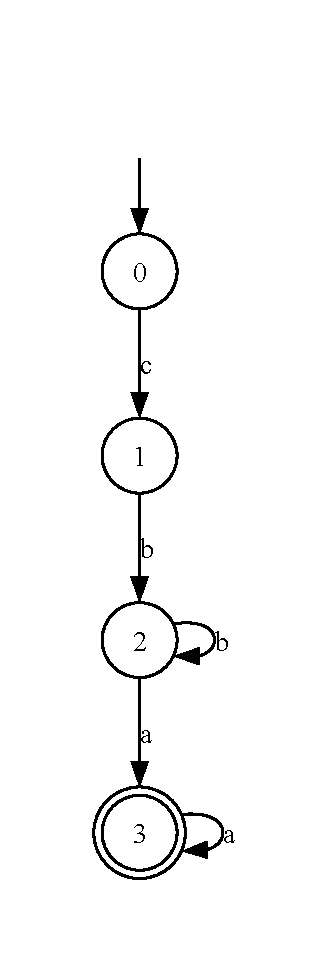
\includegraphics[keepaspectratio, scale=0.5]{reverse_regex.pdf}
%   \caption{\dfa $\aut_{cb^+a^+}$, serving as a basis for constructing $\ftEndMarker$.}
%   \label{fig:end_marker_dfa}
% \end{wrapfigure}

$\aut_{\reverse{\pi}}$ accepts $\reverse{\pi}$, but for replace operations, we need the $\ftRegexRelucAll$ to read any $x \in \Sigma^*$ and replace only the requested pattern, leaving the rest of $x$ unmodified.
Therefore, we \emph{generalize} $\aut_{\reverse{\pi}}$, producing $\aut^{\text{gen}}_{\reverse{\pi}}$, which accepts any word $x \in \Sigma^*$.
Think of $\aut^{\text{gen}}_{\reverse{\pi}}$ as the input tape of an \nft which needs to read any word on its input, and only perform a specific operation (replacement here) for a specified pattern in the input word.

Given $\aut_{\reverse{\pi}} = (\states, \Sigma, \post, \{ q_0 \}, \finalStates)$, we construct $\aut^{\text{gen}}_{\reverse{\pi}} = (\states^{\text{gen}}, \Sigma, \post^{\text{gen}}, \{ s_0 \}, \finalStates^{\text{gen}})$ where $\states^{\text{gen}} = \{ t \,\mid\, t \subseteq \states \}$ following these rules:\newline
We define a bijective mapping $\mathcal{M}: \states^{\text{gen}} \rightarrow 2^{\states }$ such that $\forall s \in \states^{\text{gen}}, a \in \Sigma: s' \in \post^{\text{gen}}(s, a)$
iff $\mathcal{M}(s') = \{ q_0 \} \cup \{ q' \,\mid\, \exists q \in \mathcal{M}(s): q' \in \post(q, a) \}$
and $\mathcal{M}(s_0) = \{ q_0 \}$.

Intuitively, we construct a new \dfa from $\aut_{\reverse{\pi}}$ where each state $s$ maps to a set of states in $\aut_{\reverse{\pi}}$ which can be reached from $q_0$ with the same substrings of $\langof{\aut_{\reverse{\pi}}}$.
Since $\aut_{\reverse{\pi}}$ is deterministic, each substring will end in at most one state $s$.
Thus, $\aut^{\text{gen}}_{\reverse{\pi}}$ remains deterministic.

However, when we encounter state $s$ where $\finalStates \cap \mathcal{M}(s) \neq \emptyset$, we know that we have reached a state in the constructed $\aut^{\text{gen}}_{\reverse{\pi}}$ where the substring corresponding to $s$ is accepted by $\aut_{\reverse{\pi}}$.
That means that we have reached an end of an accepted word in $\aut_{\reverse{\pi}}$ which we want to mark (insert an end marker $\marker$ after this substring).
Therefore, during the construction, we create a new final state $s_f$, and each time we encounter such a state $s$, we add a transition $\move{s}{\epsilon}{s_f}$, and redirect all transitions which would normally go from $s$ to start in $s_f$.
Thus the only outgoing transition from $s$ is the epsilon transition and we did not introduce a non-determinisctic choice of transitions from $s$.
Then, all states except for states $s$ where $\finalStates \cap \mathcal{M}(s) \neq \emptyset$ are made final since we want to accept any arbitrary input.
We omit the original final states since reaching these states is a significant event in reading an arbitrary input which we need to handle separately.

$\aut^{\text{gen}}_{\reverse{\pi}}$ represents an \dfa which states how ''far'' into $\reverse{\pi}$ we are when reading an arbitrary input.
Each symbol either resets the \dfa (simulating manual backtracking) to some previous matched state or all the way up to $s_0$ (no even partial match was found, we start from the beginning of the pattern), or advances to the next state in the \dfa following the pattern.

Now, $\aut^{\text{gen}}_{\reverse{\pi}}$ accepts any string $x$ on its input.
During the run of $x$ on $\aut^{\text{gen}}_{\reverse{\pi}}$, each time an end of a substring $x_2$ is encountered where $x_2 \in \reverse{\pi}$ and $x = x_1 x_2 x_3$, an epsilon transition is taken.
If we were to insert $\marker$ into $x$ each time an epsilon transition is taken, we would modify $x$ in such a way that the word would remain the same, only interspersed with $\marker$ after each end of $x_2$ (since $\aut^{\text{gen}}_{\reverse{\pi}}$ is deterministic, no other transition can be taken from the source state of the epsilon transition).
These $\marker$ represent the end markers we want to insert with $\ftEndMarker$.

See Figure~\ref{fig:generalized_end_marker_dfa} showing a generalized modification of \dfa $\aut_{cb^+a^+}$, $\aut^{\text{gen}}_{cb^+a^+}$.
For example, a word $cbcbba\marker a\marker a\marker bcb$ would be accepted by this automaton where the imaginery string symbol $\marker$ symbolically represents places where an epsilon transition was taken in the automaton.

% \begin{wrapfigure}{r}{0.3\textwidth}
%   \centering
%   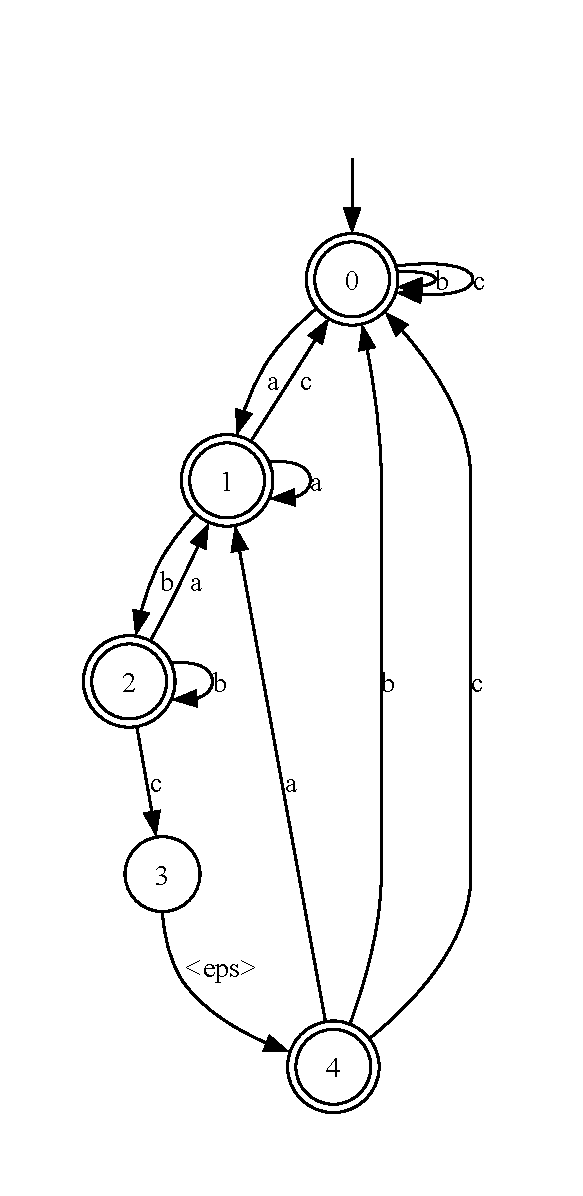
\includegraphics[keepaspectratio, scale = 0.5]{generalized_end_marker.pdf}
%   \caption{\dfa $\aut^{\text{gen}}_{cb^+a^+}$, a generalized version of $\aut_{cb^+a^+}$.}
%   \label{fig:generalized_end_marker_dfa}
% \end{wrapfigure}

Next, we can construct $\ftEndMarker$ from $\aut^{\text{gen}}_{\reverse{\pi}}$.
We simply consider the current transitions as the input tape of $\ftEndMarker$,
and we add transition symbols for output tape: for all $a \in \Sigma$, the symbol on the output tape is $a$ again, only for input symbol $\epsilon$, the output symbol is $\marker$.

We can see the final $\ftEndMarker$ for $\aut^{\text{gen}}_{cb^+a^+}$ in Figure~\ref{fig:generalized_end_marker_dft}.
% \vspace*{-1cm}
\begin{figure}[ht]
    \centering
    \subfloat[
      \dfa $\aut_{cb^+a^+}$, serving as a basis for constructing $\ftEndMarker$.
      \label{fig:end_marker_dfa}
    ]{{
      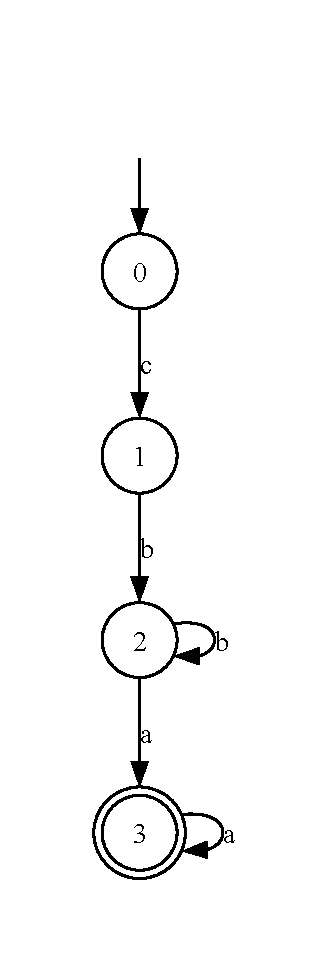
\includegraphics[keepaspectratio, width=0.2\textwidth]{reverse_regex.pdf}
    }}%
    \quad
    \subfloat[
      \dfa $\aut^{\text{gen}}_{cb^+a^+}$, a generalized version of $\aut_{cb^+a^+}$.
      \label{fig:generalized_end_marker_dfa}
    ]{{
      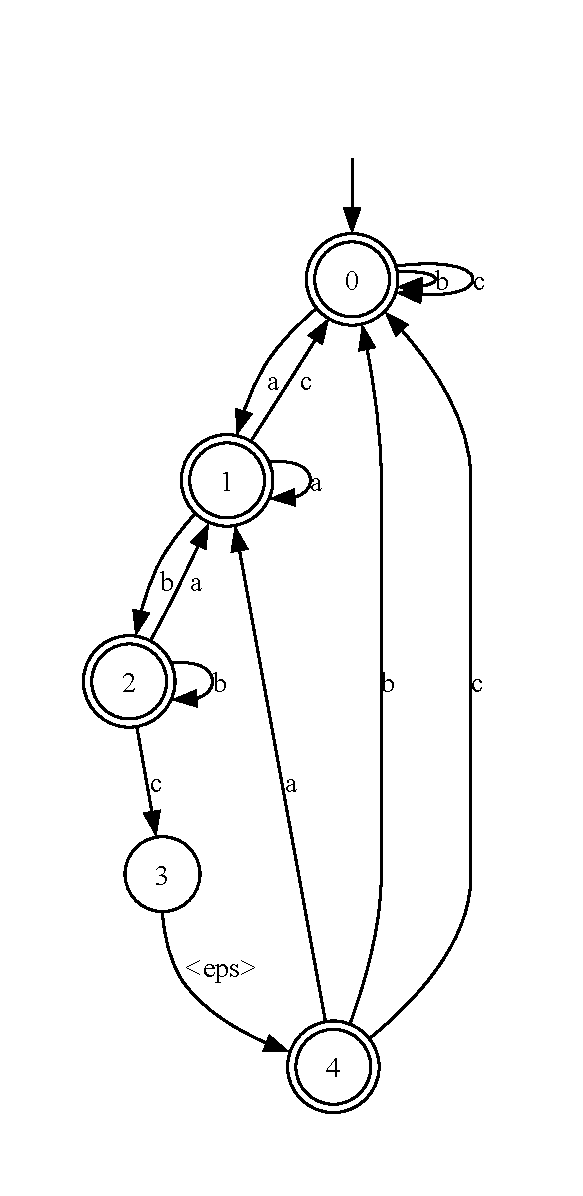
\includegraphics[keepaspectratio, width=0.33\textwidth]{generalized_end_marker.pdf}
    }}%
    \quad
    \subfloat[
      \dft $\ftEndMarker$ for $\aut^{\text{gen}}_{cb^+a^+}$ inserting the end markers $\marker$ at the correct locations in the read input word.
      \label{fig:generalized_end_marker_dft}
    ]{{
      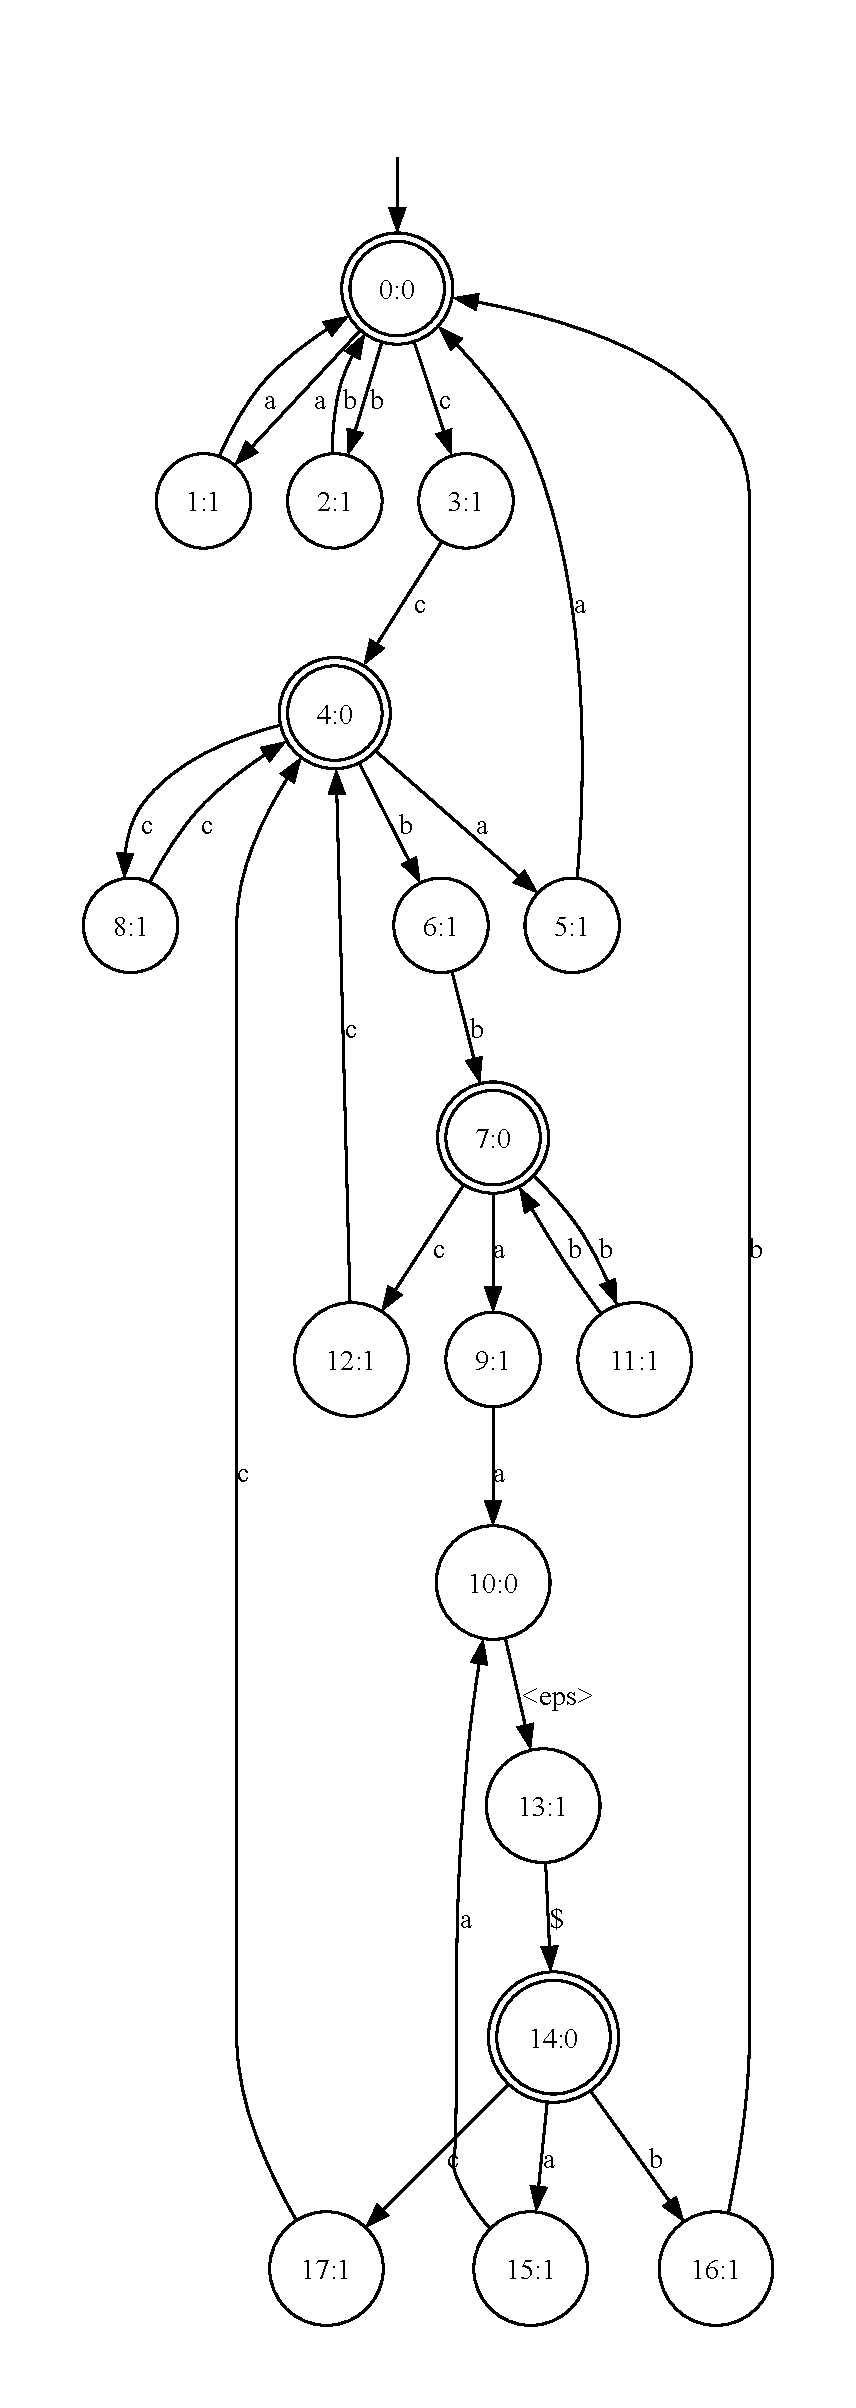
\includegraphics[keepaspectratio, width=0.33\textwidth]{end_marker_dtf.pdf}
    }}%
    \caption{
      Automata created during $\ftEndMarker$ construction.
    }
    \label{fig:end_marker_auts}%
\end{figure}

\subsection{Begin Marker \nft}

We could start constructing the \emph{begin marker} \nft $\ftBeginMarker$ from $\ftEndMarker$ by reversing all transitions in $\ftEndMarker$.
However, considering reversing a single transducer transition (consisting of operations on the input and output tapes), represented as a sequence of two \nfa transitions in \mata from state with level $0$ to $1$ and back to some state with level $0$, we instead utilize $\aut^{\text{gen}}_{\reverse{\pi}}$ before its conversion to $\ftEndMarker$ (and $\ftEndMarker$ is therefore never truly constructed in \mata).

We reverse all transitions in $\aut^{\text{gen}}_{\reverse{\pi}}$, effectively obtaining the foundation for an \nfa for marking beginnings of $\pi$.
We can now construct $\ftBeginMarker$ the same way as we constructed $\ftEndMarker$ from $\aut^{\text{gen}}_{\reverse{\pi}}$, except now $\marker$ as the output symbol for the epsilon symbol on the input tape represents the begin marker instead of the end marker.
This is why we use the same marker for symbols for both the begin and end marker, as noted earlier.
They mark the same location, only once operating on $\reverse{\pi}$, then on $\pi$.

However, marking beginnings is a non-deterministic operation.
We cannot know in advance whether the currently read symbol in an arbitrary input string marks a beginning of a full match in $\pi$.
Henceforth, we have to introduce another source of non-determinism, which gives us the smart ''look-ahead'' ability for marking beginnings for only those inputs that will later on truly match in $\pi$.
All potentially incorrectly inserted begin markers in the input word end in a non-accepting run for the word with such begin markers.
We add a new initial state $s'_0$ and add $\epsilon$ transducer transitions $\move{s'_0}{\epsilon}{s}$ ($\epsilon$ as the transition symbol on all tapes) leading to all states $s$ which are final in $\aut^{\text{gen}}_{\reverse{\pi}}$, that is, all except those which map to set of states containing the original final state from $\aut_{\reverse{\pi}}$.
The previous initial state of $\ftBeginMarker$ is set as the only final state and is removed from the initial states.

The Figure~\ref{fig:begin_marker_nft} shows a $\ftBeginMarker$ for $\reverse{\aut^{\text{gen}}_{cb^+a^+}}$.

% \vspace*{-5cm}
\begin{figure}[ht]%{r}{0.3\textwidth}
  \centering
  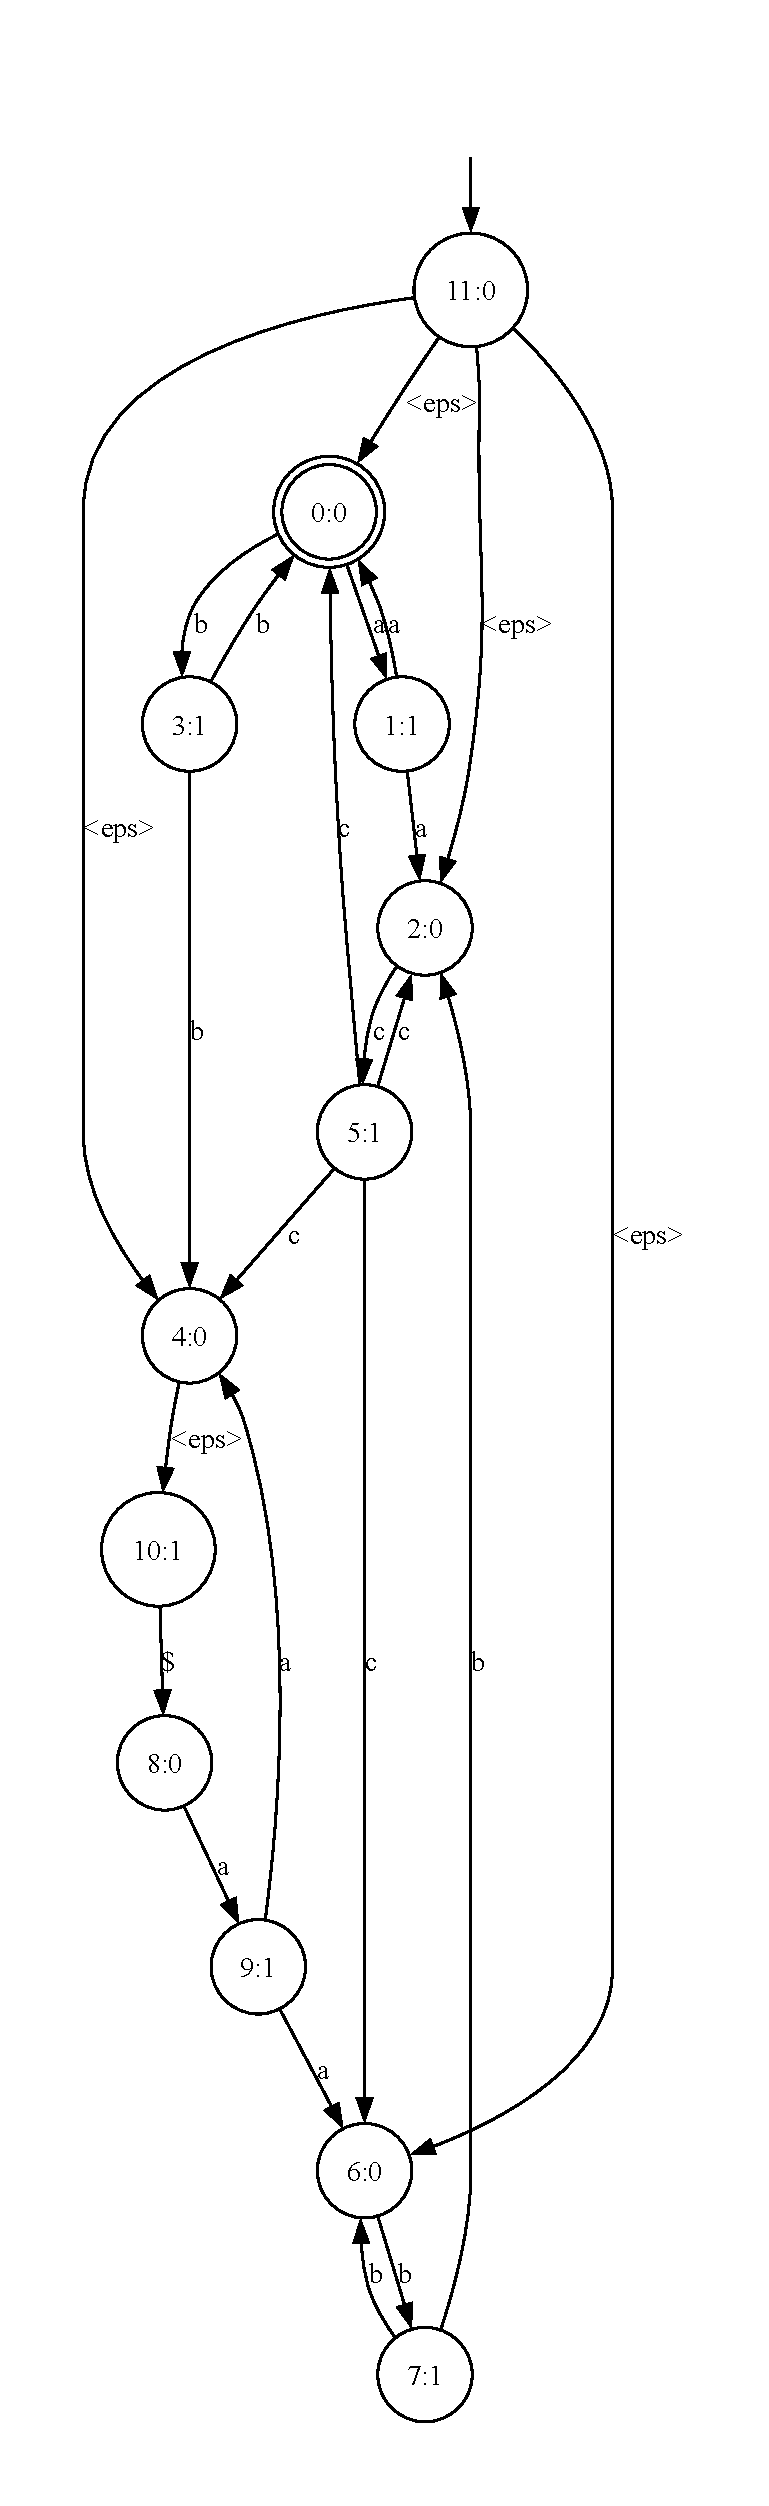
\includegraphics[keepaspectratio, scale=0.3]{nft_begin_marker.pdf}
  \caption{\nft $\ftBeginMarker$ for $\reverse{\aut^{\text{gen}}_{cb^+a^+}}$ inserting non-deterministically the begin markers $\marker$ at the beginning of matches in $a^+b^+c$ for the read input word.}
  \label{fig:begin_marker_nft}
\end{figure}

\subsection{Reluctant Replacement \nft}
\label{sec:reluctant_replacement_nft}

When we have the begin marker \nft $\ftBeginMarker$, we can construct the second \nft performing the actual replacement.
These two \nfts are used to finally construct the whole $\ftRegexRelucAll$.

We already can non-deterministically find the correct begin markers, but we now need to perform the actual replacement(s) on the input string annotated with begin markers.

We construct an \nft $\ftRegexRelucReplaceAll$ which models the actual reluctant replacement.
The idea is that we read the input string annotated with begin markers and output the same symbols unmodified on the output tape.
Once we encounter the begin marker, we know we have found the first left-most match which needs to be replaced.
Therefore, we switch to a ''replacement'' mode where we read the match without outputting anything, removing all symbols of the match and all additional begin markers inside the match.
After the match is read, we can insert the replacement for the match onto the output tape.
When the replacement is inserted, we return to the beginning to potentially perform replacement on another match.

First, we convert the $\aut_{\pi}$ into a new \nfa $\aut^{\text{short}}_{\pi}$ which accepts (matches) only the shortest input words.
This can be easily performed by removing all outgoing transitions from all final states in $\aut_{\pi}$.
Clearly,
$$\langof{\aut^{\text{short}}_{\pi}} = \{ u \in \langof{\aut_{\pi}} \,\mid\, \neg \exists u', v \in \Sigma^*: u' \in \langof{\aut_{\pi}}^{<|u|} \land u = u'v \land v \neq \epsilon \}\text{.}$$

$\aut^{\text{short}}_{\pi}$ now matches the shortest words in the language of $\aut_{\pi}$, but does not allow skipping over additional $\marker$ encountered during the reading of the match.
Such $\marker$ need to be skipped since $\marker$ inside the shortest left-most match represent beginnings of potential matches further to the right than the left-most match.
We need to therefore add a self loop to every state in $\aut^{\text{short}}_{\pi}$ with transition symbol $\marker$.

Now, the final modification is to keep the next begin marker for the next shortest left-most match. $\aut^{\text{short}'}_{\pi}$ can be constructed given $\Sigma^*_\marker = \Sigma^* \cup \{ \marker \}$ as $\aut^{\text{short}'}_{\pi} = \aut^{\text{short}}_{\pi} \cap \overline{\Sigma^*_\marker \concat \{ \marker \}}$.

$\aut^{\text{short}'}_{\pi}$ can be converted into $\ft^{\text{short}'}_{\pi}$ where the existing transitions are the input tape transitions, and the output symbols are all $\epsilon$ (\nft only reading the input word---the match---and consuming the whole match including $\marker$ inside the match).

Figure~\ref{fig:ft_regex_reluc_replace_all} symbolically shows how to construct $\ftRegexRelucReplaceAll$ for replacing all shortest left-most occurrences of regular language $\pi$ with $y$.

To replace only one occurrence (the first shortest left-most match), a variation of $\ftRegexRelucReplaceAll$, $\ftRegexRelucReplaceSingle$ can be constructed, as seen in Figure~\ref{fig:ft_regex_reluc_replace_single}.
Here we do not return to the beginning after the first replace, but move to a new state with just reads the rest of the word unmodified while removing the additional $\marker$.

% \vspace*{-1cm}
\begin{figure}[ht]
    \centering
    \subfloat[
      Symbolic representation of $\ftRegexRelucReplaceAll$ for replacing all shortest left-most occurrences of $\pi$ with $y$. All occurrences of $\pi$ are being replaced.
      \label{fig:ft_regex_reluc_replace_all}
    ]{{
      \includegraphics[keepaspectratio, width=0.45\textwidth]{{jumps_synchronization-regex_reluctant_replace_all.pdf}}
    }}%
    \quad
    \subfloat[
      Symbolic representation of $\ftRegexRelucReplaceSingle$ for replacing single shortest left-most occurrence of $\pi$ with $y$. the remaining occurrences of $\pi$ are left unmodified.
      \label{fig:ft_regex_reluc_replace_single}
    ]{{
      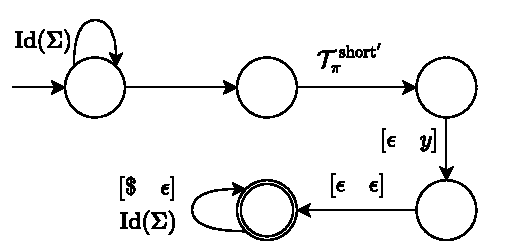
\includegraphics[keepaspectratio, width=0.45\textwidth]{jumps_synchronization-regex_reluctant_replace_single.pdf}
    }}%
    \caption{
      Symbolic representations of $\ftRegexRelucReplaceAll$ and $\ftRegexRelucReplaceSingle$.
    }
    \label{fig:regex_reluc_replace_all_single}%
\end{figure}

\subsection{Whole Regex Reluctant Replace \nft}

We have constructed $\ftBeginMarker$ to insert non-deterministically begin markers into the input word and constructed $\ftRegexRelucReplaceAll$ (or $\ftRegexRelucReplaceSingle$) to perform the replacement upon encountering matches prepended with $\marker$.
$\ftRegexRelucAll$ (and similarly $\ftRegexRelucSingle$) can be constructed by connecting these two \nfts into a sequence using composition: $\ftRegexRelucAll = \ftBeginMarker \composePipe \ftRegexRelucReplaceAll$ and $\ftRegexRelucSingle = \ftBeginMarker \composePipe \ftRegexRelucReplaceSingle$.
$\langof{\ftRegexRelucAll} = \{ (u, v) \in \Sigma^* \times \Sigma^* \,\mid\, v = u^{+}_{\pi \rightarrow y} \} $ and $\langof{\ftRegexRelucSingle} = \{ (u, v) \in \Sigma^* \times \Sigma^* \,\mid\, v = u^{1}_{\pi \rightarrow y} \} $.

\section{Transducers for Literal Reluctant Replacement}

Constructing \nfts for regex reluctant replacement is expensive.
Therefore, when the \texttt{pattern} to be replaced is of a simpler form, namely a string literal, or even a single symbol, a corresponding \nft for reluctant replacement can be constructed faster.

\subsection{Single Symbol Replacement}

We can construct a replacement \dft for a single symbol reluctant replacement by creating a single-state \dft with $\id{\Sigma}$ self-loop transducer transitions.
Then only modify the output transition for the input symbol by replacing it with a transition (or a sequence of transitions) outputting $y$ on the output tape ($y$ can be either a single symbol or a literal) to produce the replacement.
The handling of all and single reluctant replacement variations is the same as for regex reluctant replacement: we either return to the original state, or create a new final state with $\id{\Sigma}$ self-loop transitions.

\subsection{Replacement of Finite String Literal}

To construct an \nft for the replacement of a string literal $z$ with $y$, we need to construct two \nfts.

First, we want to annotate the end of the input words $x$ similarly to how $\ftEndMarker$ annotates the end of the patterns, but now a simple \nft $\ft_\marker$ with an initial state $q_0$, final state $q_f$, and transitions $(q_0, \id{\Sigma}, q_0)$, and $(q_0, (\epsilon, \marker), q_f)$ will suffice. $(u, u\marker) \in \langof{\ft_\marker}$.

Second, we need to construct an \nft $\ftLiteralRelucReplaceAll$ for replacing all literals, or $\ftLiteralRelucReplaceSingle$ for replacing only the first left-most shortest literal.

$\ftLiteralRelucReplaceAll = (\states, \Gamma, \post, \{ q_0 \}, \{ q_f \})$ can be constracted using the following method.
We construct an \nft for $z$ where $z$ represents the input tape and a sequence of $\epsilon$ symbols represents the corresponding output tape.
Each state $q$ uniquely maps to its corresponding substring of $y$: $\mathcal{M}: \states \rightarrow \Sigma^*$ is a bijection where $\mathcal{M}(q_0) = \epsilon$, $\mathcal{M}(q_1) = y[0:1]$, $\mathcal{M}(q_1) = y[0:2]$, $\mathcal{M}(q_2) = y[0:3]$, etc.
Each state therefore represents a ''buffer'' of symbols read so far on the input tape which have not been outputted on the output tape yet.
We already have transitions as constructed from $z$ for each state.

Now we add additional transitions as follows:\newline
\begin{itemize}
  \item If $\marker$ is read on the input tape, we output the contents of the buffer $\mathcal{M}(q)$ where $q$ is the current state (symbols read from the input word but not outputted onto the output tape yet) and move to $q_f$.
  \item If $a \in \Sigma$ and $z = \mathcal{M}(q) \concat a$ ($a$ is the last symbol in $y$), we perform the replacement: outputting $y$, and move to the beginning $q_0$ to continue replacing the next match.
  \item If $a \in \Sigma$ and $a \neq z[|\mathcal{M}(q)|:|\mathcal{M}(q)| + 1]$ ($a$ is not the next symbol in $z$---those transitions are already in  $\ftLiteralRelucReplaceAll$), we determine the longest prefix $p$ of $z = pv$ such that $up = \mathcal{M}(q) \concat a$ from left to right.
  We output $u$ onto the output tape (as a sequence of transition symbols) and move to state $q' = \mathcal{M}(p)$ which represents the longest prefix of $z$ currently being ''buffered'' and not processed yet.
\end{itemize}

When constructing $\ftLiteralRelucReplaceSingle$, instead of moving to $q_0$ after reading $z$ and outputting the replacement $y$, we move to a final state $q_f$, and add transitions to simply read the rest of the input word and output the word unmodified onto the output tape, removing $\marker$ at the end: $(q_f, \id{\Sigma}, q_f)$ and $(q_f, (\marker, \epsilon), q_f)$.

To construct $\ftLiteralRelucAll$ (or $\ftLiteralRelucSingle$), a composition of $\ft_\marker$ and $\ftLiteralRelucReplaceAll$ (or $\ftLiteralRelucReplaceSingle$) is performed: $\ftLiteralRelucAll = \ft_\marker \composePipe \ftLiteralRelucReplaceAll$ or $\ftLiteralRelucSingle = \ft_\marker \composePipe \ftLiteralRelucReplaceSingle$.

\begin{example}
  For literal reluctant all replacement $x^{+}_{cc  \rightarrow a}$, we can see that $\mathcal{M}(0) = \epsilon$, $\mathcal{M}(1) = c$, $\mathcal{M}(2) = cc$.

  Figure~\ref{fig:literal_reluctant_replace} shows both variations (replace all and replace single) \nfts for $x^{+}_{cc \rightarrow a}$.

  Thanks to our approach, $\ftLiteralRelucAll$ and $\ftLiteralRelucSingle$ maintain the same structure after composition as $\ftLiteralRelucReplaceAll$ and $\ftLiteralRelucReplaceSingle$.
  The only difference is that marker symbols $\$$ are replaced with $\epsilon$.

\begin{figure}[ht]
    \centering
    \subfloat[
      $\ftLiteralRelucReplaceAll$ for replacement $x^{+}_{cc  \rightarrow a}$.
      \label{fig:literal_reluctant_replace_all}
    ]{{
      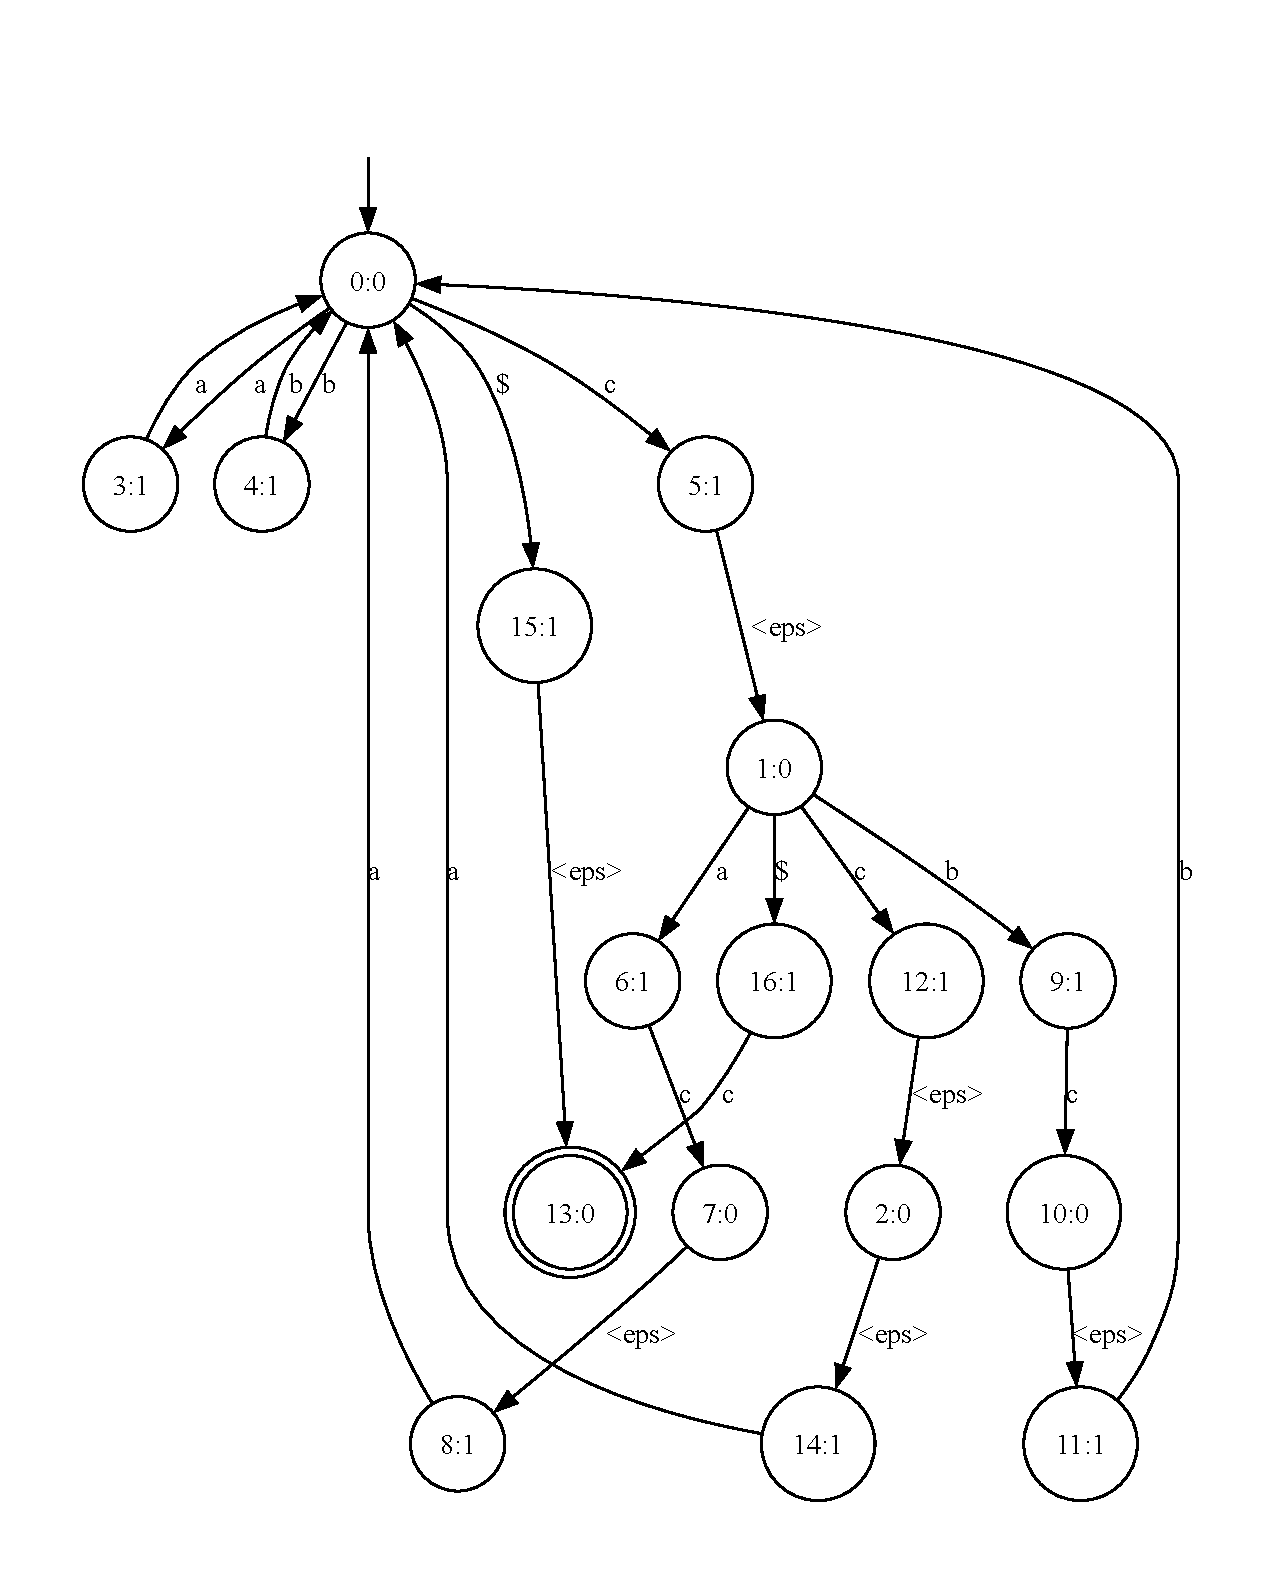
\includegraphics[keepaspectratio, width=0.50\textwidth]{reluctant_replace_literal_all.pdf}
    }}%
    \quad
    \subfloat[
      $\ftLiteralRelucReplaceSingle$ for replacement $x^{1}_{cc  \rightarrow a}$.
      \label{fig:literal_reluctant_replace_single}
    ]{{
      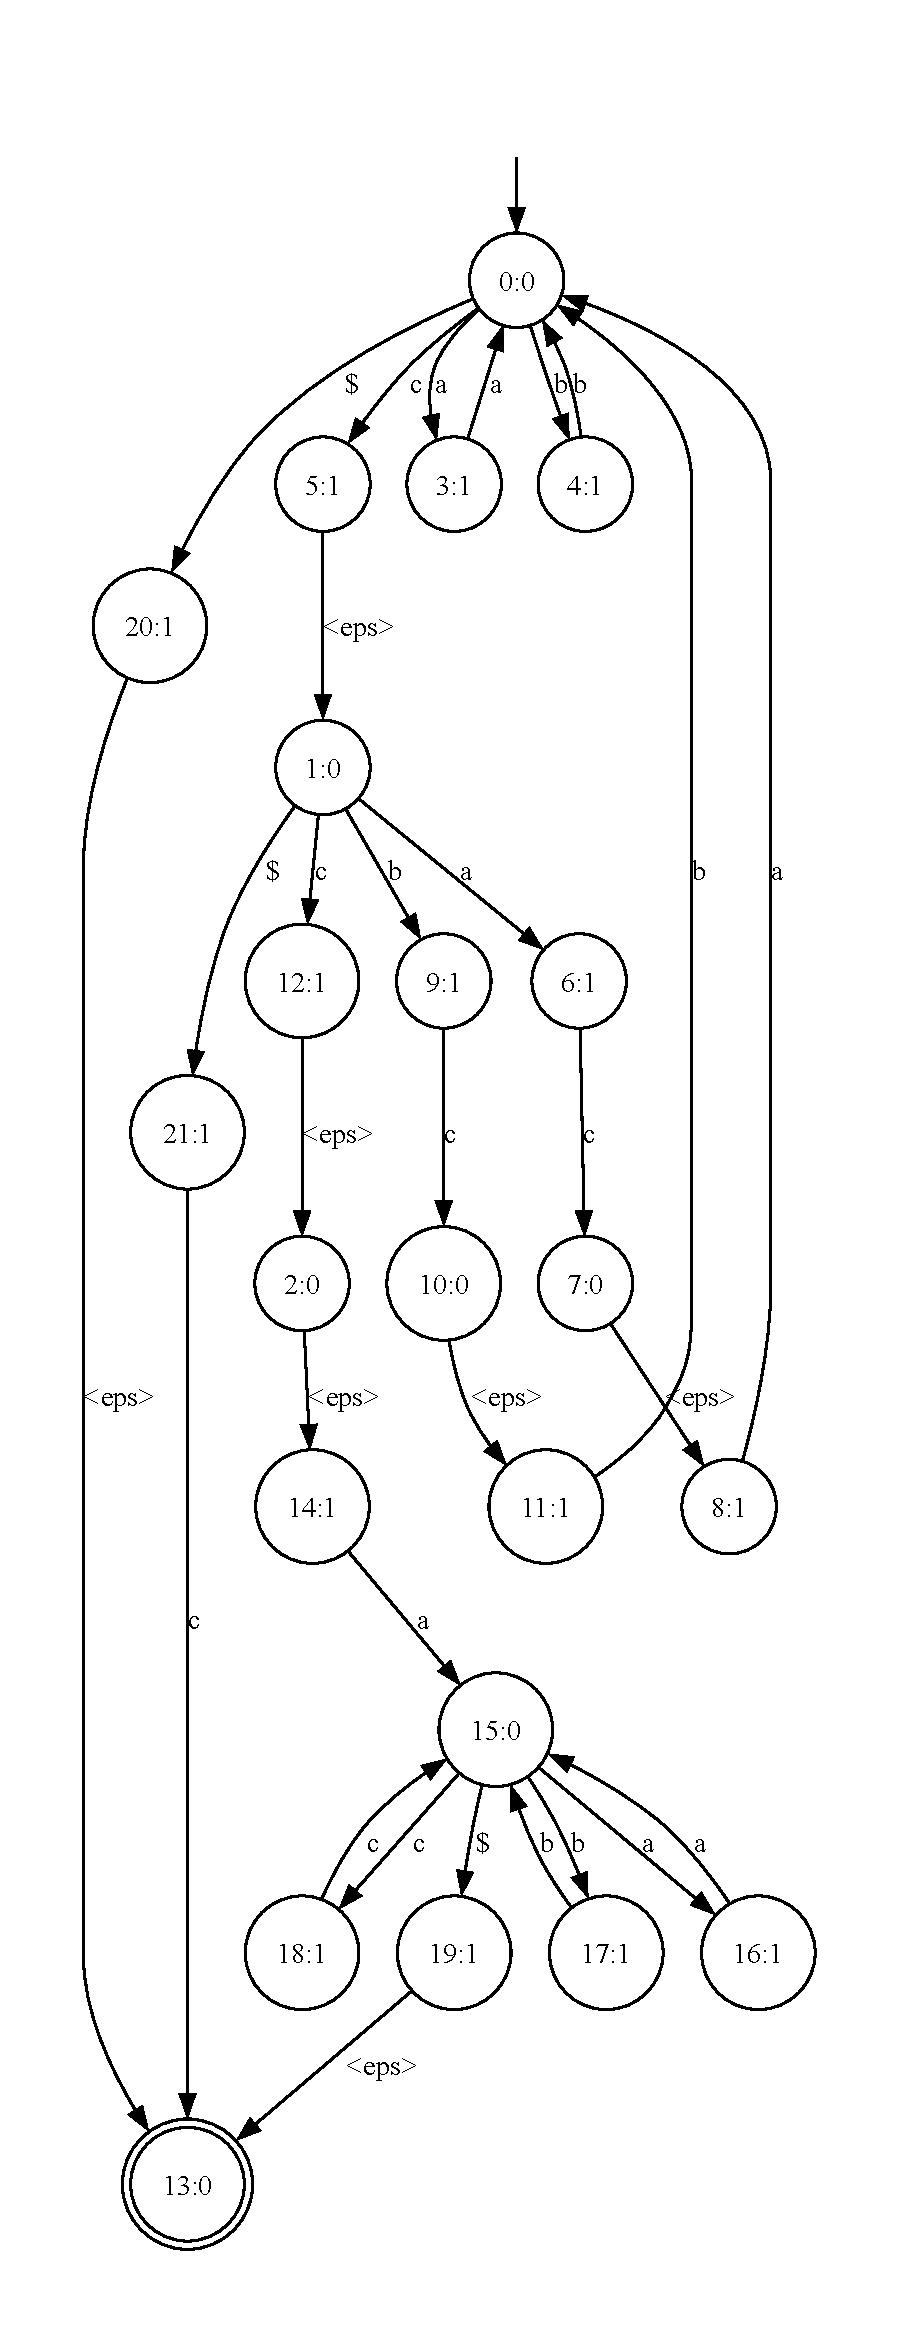
\includegraphics[keepaspectratio, width=0.33\textwidth]{reluctant_replace_literal_single.pdf}
    }}%
    \caption{
      $\ftLiteralRelucReplaceAll$ and $\ftLiteralRelucReplaceSingle$ for $x^{+}_{cc \rightarrow a}$ and $x^{1}_{cc \rightarrow a}$ replacements.
    }
    \label{fig:literal_reluctant_replace}%
\end{figure}

\end{example}

Note that this approach could be generalized to a regex replacement where the regex has finite length, similarly to how~\cite{replace_nfts_model_ModelingRegularReplacementForStringConstraintSolving_DBLP:conf/nfm/FuL10} models finite regex replacements.
However, for our uses in \noodler, we currently do not solve any industry benchmarks where finite regex replacement occurs.
Further, when modelling finite regex replacement for regex $\pi$ with the maximal length $n$ of a string $u \in \langof{\pi}$, one needs to create states for all possible substrings of $\Sigma^{\leq n}$, each with the transitions similar to those in $\ftLiteralRelucAll$.
This is computationally costrly and the constructed state space increases dramatically.

\section{Solving SMT Formulae with Replace Operations}
\label{sec:string_solving_with_replace}

The main decision procedure of \noodler rewrites SMT formulae into a form where the formula contains regular constraints (where both the variables and the regular constraints have assigned regular languages) and \noodler checks whether the languages for variables after restricting the languages by the string constraints are non-empty.
If during the procedure a language of some variable becomes empty, there is no assignment for the formula which could assign the variable a word satisfying the constraints.

The formulae solved by \noodler which contain replace operations always follow the following general structure:
$$ x \in \ldots \land u = \texttt{replace}(\ldots (\texttt{replace}(\texttt{replace}(x, \pi_1, y_1), \pi_2, y_2)\ldots), \pi_n, y_n) \land u \in \ldots \text{.}$$

We have a sequence of nested replace operations.
There can be between one and about 200 nested replace operations on the benchmarks from industry solved by \noodler, usually working with small tens of unique transition symbols\footnote{This is thanks to that our decision procedure in \noodler substitutes transition symbols not explicitly worked with in the formula with just two ''dummy'' transition symbols.}.

\begin{example}\label{ex:smt_replace_sequence}
  An encoding for operation \texttt{toUpper} which replaces all lowercase letters in $x$ with uppercase letters looks like this:
  $$ x \in \ldots \land u = \texttt{replace}(\ldots (\texttt{replace}(\texttt{replace}(x, `\text{a}`, `\text{A}`), `\text{b}`, `\text{B}`)\ldots), `\text{z}`, `\text{Z}`)\land u \in \ldots \text{.}$$.

  Another often performed operation is \texttt{HTMLEscape} which properly escapes special HTML symbols from the input string $x$ so as not to break the HTML when the user input gets inserted into the HTML webpage:
  \begin{multline*}
  x \in \ldots \land u = \texttt{replace}(\ldots (\texttt{replace}(\texttt{replace}(x, `\text{<}`, ``\text{\&lt;}``), `\text{\&}`, ``\text{\&amp;}``)\ldots), \\
  \texttt{from\_code}(39), ``\text{\&\#39;}``)\land u \in \ldots
  \end{multline*}
  where \texttt{from\_code}($n$) performs a conversion from integer code $n$ to its corresponding Unicode character.

  And finally, there are operations working with regexes $\pi$:
  $$
    x \in \ldots \land u = \texttt{replace}(x, ``\texttt{.d}^+\texttt{.}``, ``\text{\_\$1}``)\land u \in \ldots
  $$
where regex $``\texttt{.d}^+\texttt{.}``$ represents a regex describing one or more occurrences of \texttt{d} surrounded by one character from both sides. For example \texttt{adde} matches, but \texttt{aed} does not.

All of these examples come with variants for replacing all or only the first occurrence of the regex or literal, and with varying number of nested replacements.

The general approach to extend string solvers with support for replace operations and string transformations in general has already been pioneered in the context of monadic decomposition-based algorithms, as seen in~\cite{AnthonyReplaceAll2018, Flatten, ChainFree, StringAFA}.
However, adding this support for \noodler for its stabilization decision procedure is a challenging task with interesting qualities.

\end{example}

As seen in Example~\ref{ex:smt_replace_sequence}, we often reason about regular languages for both the input and output language of a sequence of nested replace operations.
Internally in \noodler, each level of the nested hierarchy will get assigned a new fresh variable $x_i$, so we obtain from
$$
x \in \ldots \land u = \texttt{replace}(\ldots (\texttt{replace}(\texttt{replace}(x, \pi_1, y_1), \pi_2, y_2)\ldots), \pi_n, y_n) \land u \in \ldots \text{.}
$$
a formula similar to
\begin{multline*}
x \in \ldots \land u_1 = \texttt{replace}(x, \pi_1, y_1) \land u_2 = \texttt{replace}(u_1, \pi_2, y_2) \land \ldots \land \\u = \texttt{replace}(u_{n-1}, \pi_n, y_n) \land u \in \ldots \text{.}
\end{multline*}

Since we need to propagate the properties of $x$ over all the replace operations to $u$, we need a method to propagate the information over the replace operation.
Remember that now we consider both $u$ and $x$ to be string variables with an assigned regular language, $\langof{u}$ and $\langof{x}$.
The problem can be therefore split into smaller problems of form $ u = x^{+}_{\pi \rightarrow y}$ (representing a single replace operation from above) and propagating the information from $x$ to $u$.

In string solving, we work with \nfts with two tapes: the input tape and the output tape.
Thefore, we define $\projInput{\ft}$ and $\projOutput{\ft}$ as special cases of projections, performing $\projToSet{\{ 0 \}}{\ft}$ and $\projToSet{\{ 1 \}}{\ft}$, respectivelly.
Performing projection on either tape produces an \nfa representing the language of the corresponding tape.
The projection of \nft $\ft$ to its output tape, $\projOutput{\ft}$, gives us the forward image of $\ft$, \nfa $\aut_{\text{out}}$.
Similarly, the projection of \nft $\ft$ to its input tape, $\projInput{\ft}$, gives us the backward image of $\ft$, \nfa $\aut_{\text{in}}$.

For the given problem $ u = x^{+}_{\pi \rightarrow y}$ with $\aut_x$ and $\aut_u$ being the \nfas representing the regular languages assigned to variables $x$ and $u$, we can compute the language (the corresponding \nfa) of the forward image as $\projOutput{\idNft{\aut_x} \composePipe \ft_{x^+_{\pi \rightarrow y}}}$, i.e., the forward application (propagation) of $\aut_x$ on $\ft_{x^+_{\pi \rightarrow y}}$ which gives us the admissible $\langof{u}$ for the given $\langof{x}$.
The backward image can be computed as $\projInput{\ft_{x^+_{\pi \rightarrow y}} \composePipe \idNft{\aut_u}}$, that is, backward application (propagation) of $\aut_u$ on $\ft_{x^+_{\pi \rightarrow y}}$ which gives us the admissible $\langof{x}$ for the given $\langof{u}$.

\paragraph{Languages of variables as concatenations of regular languages}
A decision procedure in \noodler, called \emph{stabilization}~\cite{oopsla23_stabilization_DBLP:journals/pacmpl/ChenCHHLS23}
performs automata operations on languages for variables which may be represented as a concatenation of multiple regular languages for other variables.
For an algorithm called \emph{noodlification} performed as a part of this procedure, we need to concatenate these languages with special epsilon symbols (different from those used in construction of \nfts for replace operations).
Therefore, we need to handle these symbols during replace operations as regular symbols, not epsilon symbols, in order to maintain a clear separation of languages of each individual variables in the concatenation.\footnote{The epsilon nature of these special symbols is utilized only in noodlification to indicate move between languages of variables in the concatenated language.}.

\paragraph{Flattening of the nested hierarchy of replace operations.}
To further optimize the computation of $u$ from $x$ through a nested hierarchy of replace operations, one can precompute $\ft_\text{seq}$ as a sequential composition of all \nfts for the corresponding replace operations.

Then, the hierarhcy is flattened into a single $\ft_\text{seq}$ performing all the replace operations simultanously: $u = \ft_\text{seq}(x)$.

Note that in the benchmarks solved by \noodler, the patterns being replaced are unique in that the replacement of one \nft is never later in the sequence matched to the pattern of another \nft.
E.g., operation \texttt{toUpper} performs sequence of transductions, each matching one of the lowercase letters of the alphabet and replacing it with its uppercase version.
It never happens that the uppercase letter replacing the lowercase one is later replaced with some other letter.
Therefore, an optimization of flattening a sequence of transducers satisfying this property can be utilized: the transductions in the whole sequence are associative.
We can construct intermediate \nfts for composition of any combination of \nfts in the sequence, disregarding the order of the \nfts in the sequence to more quickly construct the final \nfts for the whole sequence.
The reason for why the nested hierarchy is necessary for SMT formulae encoded in SMT-LIB format is that since the SMT-LIB format does not allow specifying a single replace operation with multiple (\texttt{pattern}, \texttt{replacement}) pairs, performing operations such as \texttt{toUpper} can be encoded only as a sequence of independent replacements which is however an unoptimal encoding for SMT solvers, especially those which can utilize the abilities of \nfts for the representation of replace operations.

\paragraph{Length constraints.}
Some variables may be length constrainted in addition to the string constraints.
Length constraints for variables are in \noodler solved separately using a LIA (linear integer arithmetic) solver provided by \ziii.
If the variables $u$ and $x$ are length variables, we need to maintain the information about lengths through the replace operation (which can in general change the length of words between $u$ and $x$).
To propagate lengths of words through the replace operations, an option would be to compute an existential Presburger formula $\phi$ based on a computation of a Parikh image of $x^{+}_{\pi \rightarrow y}$, as described in~\cite{ChainFree}.

We compute the standard Parikh image~\cite{DBLP:conf/icalp/SeidlSMH04} on the \nft for replace operation with the whole $n$-tuples of transition symbols being handled as single macrosymbols (obtaining an \nfa over the language of said $n$-tuples).
$\phi$ now encodes the relationship between the number of occurrences of $n$-tuples (macrosymbols) in $s \in \langof{\ft_{x^{+}_{\pi \rightarrow y}}}$.
To get the relationship between the actual letters $a \in \Sigma$ inside the $n$-tuples $\alpha$, we must extend $\phi$ with variables $a_i$ counting the number of occurrences of each $a$ on each tape $i$ ($i$-th element of $\alpha$), and compute the relationship between each $a_i$ and $\#\alpha$, representing the number of $\alpha$ symbols in the Parikh image, as: $a_i = \sum_{\alpha \in \Sigma^n_{\epsilon}: \alpha[i] = a} \#\alpha$ where it must hold that $|x_i| = \sum_{a \in \Sigma} a_i $ is the length of words on each tape $i$.

% TODO: What needs to be modified.
The existing decision procedure of \noodler will have to be modified further as follows:
\begin{itemize}
  \item Adding saturation of replace operations, similarly to how \noodler saturates other string functions,
  \item Inclusion graph~\cite{fm23_equations_synergy_regular_constraints_DBLP:conf/fm/BlahoudekCCHHLS23} used by \noodler will have to be extended to support replace operations.
\end{itemize}

\chapter{Implementation}

The proposed data structures for finite transducers, standard operations on finite transducers, and algorithms for modelling replace operations were implemented in \mata.
The code is accessible in a \href{https://github.com/Adda0/mata/tree/transducers}{GitHub repository}\footnote{\url{https://github.com/Adda0/mata/tree/transducers}} and will be merged into the main \mata \href{https://github.com/VeriFIT/mata/}{GitHub repository}\footnote{\url{https://github.com/VeriFIT/mata/}}.

The majority of the operations on finite transducers closely follow the implementation of the corresponding operations on \nfas already existing in \mata.
These operations are modified only in places where it is necessary to handle the differences between \nfas and \nfts, such as correctly setting and resetting the vector of levels for transducer states, or handling epsilon, \nop and don't care symbols.

Furthermore, several algorithms specific for \nfts are added to \mata, namely composition of two \nfts, application (of both an \nfa and a word) on an \nft, projection (to a specified subset of \nft tapes---producing a new \nft---or to only a single tape---producing the corresponding \nfa for the specified tape).

\paragraph{Levels.}
The vector of levels is a vector of unsigned integers representing the levels indexed by states.

Each \nft also stores the number of tapes (levels) in the \nft.
The number of tapes defaults to $1$, which means that the \nft is equivalent to \nfa and the operations on \nfts with number of levels set to $1$ will behave the same as a corresponding \nfa (with an equivalent transition relation where all don't care transitions are replaced with transition between the same states over the whole alphabet).

This is useful as it keeps the data structures in \mata consitent with the behaviour expected by many potential users of \mata.

\paragraph{Epsilon and no operation transitions.}
We have decided to unify the symbols for epsilon transitions and \nop transitions used in \mata.
We represent both transitions with a transition over an epsilon symbol $\epsilon$, corresponding to the largest unsigned integer value of a symbol in \mata.

To distinguish between both, we check whether the epsilon transition leads from a state with level $k$ to a state with level $k + 1 \mod n$ or not whenever we encounter the symbol in algorithms.
This operation has constant complexity since a set of levels in \mata is a state-idexable vector of levels.

We decided for this approach since all operations in \mata already support epsilon transitions, checking for existence of epsilon transitions and accessing them has constant complexity, and adding handling for yet another special transition symbol further complicates the logic for many operations which do not have to distinguish between epsilon and no operation transitions.

\paragraph{Words and identity insertion.}
We also implemented a few utility functions which are useful when constructing or modifying \nfts\footnote{Especially during construction of \nfts for the replace operations and other often used operations in string solving.} such as
\begin{itemize}
  \item \emph{inserting an identity transition} over all tapes (all tapes read/write the same symbol) over the given alphabet for a specified state.

  This is specially useful for string solving where usually one specially handles a small subset of transitions symbols, but wants to leave the remaining symbols in the input word unmodified.

  \item \emph{inserting a word} for specified tapes or \emph{inserting words}, one for each tape.

  This allows one to quickly create transducers which read a specific word, replace a specific string literal with a given literal, or remove a specified literal from the input word.
\end{itemize}

\paragraph{Specifying tapes to work on.}
Since we aim to implement \nfts in \mata so they are usable for general purposes, not only limited to string solving, we allow for the majority of operations to specify what is the interpretation of each tape: e.g., which tapes are to be the input tapes, and which are to be the output tapes in application of a word or a language; or which tape(s) to use for synchronization during composition.

Be mindful that using different tapes for some operations may affect the performance of these operations. For example, application on the first tape is more performant than the application on the last tape in an $n$-tape \nft.

\section{Similarities with operations on BDDs}
Since the idea of data structures and operations for \nfts in \mata was to provide the same underlying data structures as well as the interface for both \nfts and BDDs, many of the operations on \nfts and BDDs follow the same general algorithm with just slight modification in how \nfts and BDDs interpret the same instance of an \nft automaton.
For example, when using BDDs, one will interpret jumps over several levels to represent a sequence of transitions where the first transition has the transition symbol given by the jump, but the remaining transitions have $\dontCare$ symbols as opposed to the \nft interpretation where all transitions in the jump have the jump symbol.

% \paragraph{Support for BDDs.}
For the implementation of the current interface and algorithms specific for \nfts (composition and projection), I used the existing implementation for a simple prototype BDD representation using \nfas with levels (supporting simple composition and projection operations), which was implemented previously in \mata.
I further modified the interface for the existing operations, expanded the interface with new operations, added string solving-specific operations (construction of typical \nfts used in string solving, \nfts for replace operations, \ldots).
I collaborated with our colleagues to define the same interface for \nfts and future proper implementation of BDDs, inherited from \nfts.

As a result of discussions and collaboration, I add support for \nfts (this work, utilizing the existing implementations for projection and composition) and we plan adding support for BDDs in the future: using the defined common interface, where BDDs inherit operations from \nfts where the cores of the \nft- and BDD-specific operations from Section~\ref{sec:Algorithms} (composition, projection) are modified and extended versions of the existing implementations for BDD operations.

Thanks to this collaboration, we are able to add official support for BDDs into \mata easily by inheriting \nft and modifying handling of jump transitions and several additional changes.
Therefore, \nft projection will be similar to BDD projection, \nft composition similar to BDD composition, etc.
The proper support for BDDs inheriting from \nfts is planned to be implemented when the current implementation for \nfts matures enough.

\chapter{Experimental Evaluation}
\label{chap:experiments}

For our experiments, we are interested in how \mata performs when running operations on \nfts modelling the replace operations required by \noodler.
Modelling replace operations in \noodler is not the only use case for \nfts in \mata, but it is the first domain where \nfts will be used.
% Since our main indent is to use \nfts in \mata as models to replace operations in \noodler, we need to optimize the \nft algorithms primarily to this use case, while keeping the \nft algorithms general enough for other use cases.

We compare the performance of \nfts implemented in \mata with a state-of-the-art automata library \mona~\cite{mona}.

Even if \mona does not support finite transducers directly, we have chosen \mona to compare \mata against because \mona is a well-optimized library which, thanks to its ability to encode transition relation into MTBBs, provides a reasonable model for encoding finite transducers.
Each tape in a transducer can be encoded as a single variable in the BDD for a given transition.
A sequence of variables then encodes an \nft transition, where the leaves of the BDD are target states and edges represent the transition symbols.
Each transition symbol is encoded as a bit vector (a sequence of bits).
An \nft transition is then encoded as \texttt{dummy\_1|bitvec\_1|dummy\_2|bitvec\_2} where \texttt{|} denotes the concatenation of bit vectors. \texttt{bitvec\_i} represents a bit vector for a transition symbol on the tape $i$.
\texttt{dummy\_i} are additional dummy symbols used for determinization (as \mona implicitly determinizes after every operation).

Performing operations such as composition, projection, or application on \nfts is, thanks to how \mata encodes \nfts as a representation very close to the representation of BDDs, a natural operation for \mona in the encoding explained above.

Intuitively, \mata performs modified \nfa operations on \nfts while \mona performs its BDD operations with the proper encoding.

Our goal in these experiments is not to outperform \mona, but to compare how techniques for \nfts using explicit alphabets with support for nondeterminism (\mata) perform against symbolic alphabets with binary representation of transition relations (binary bit vectors in \mona) without support for nondeterminism.

\section{Benchmarks.}

For the first group of benchmarks, we have generated a new set of benchmarks from runs of \noodler on benchmarks from SMT-LIB~\cite{SMTLIB} which contain string replace operations \texttt{str.replace}, \texttt{str.replace\_all}, \texttt{str.replace\_re} and \texttt{str.replace\_re\_all}.
The replace operations appear in SMT-LIB benchmarks
\\\texttt{
non-incremental/QF\_SLIA/20230331-transducer-plus}\\(\transducerPlus, called \texttt{transducer plus} in our experiments), and\\\texttt{
non-incremental/QF\_SLIA/20230403-webapp}\\(\webapp, called \texttt{webapp} in our experiments).

We compare the performance of \mata and \mona on benchmarks for the following operations
\begin{itemize}
  \item projection to input/output tapes,
  \item application of a literal (forward/backward),
  \item application of a language (forward/backward),
  \item composition of two \nfts, and
  \item composition of \nfts used during replace \nft construction.
\end{itemize}

We collect \nfts for each unique replace operation in benchmarks from SMT-LIB solved by \noodler.
Furthermore, we extend this list by constructing \nfts for partial compositions of a sequence of replace operations (various subsequences) which appear in the SMT-LIB benchmarks.

\paragraph{Projection benchmark.}
The projection benchmark consists of unique single $2$-tape \nfts for replace operations found in SMT-LIB formulae solved by \noodler.
We perform projection to tape $0$ (projecting out the tape $1$), and projection to tape $1$ (projecting out the tape $0$).
We remove duplicated \nfts in each benchmark which in total produces $1749$ instances ($202$ from \webapp, $1547$ from \transducerPlus).

\paragraph{Application of a literal benchmark.}
The application of a literal benchmark consists of pairs ($u$, $\ft$) where $u$ is a string literal and $\ft$ is a $2$-tape \nft for replace operations found in SMT-LIB formulae solved by \noodler.
$u$ is constructed as the longest word in the \texttt{pattern} of the replace operation constrainted to the maximal length of word $5$ ($5$ is up to a few exception a sufficient length for all replace operations in SMT-LIB).
We perform the forward application of $u$ to $\ft$ ($\id{u} \composePipe \ft $).
This simulates the forward image propagation, as described in~\ref{sec:string_solving_with_replace}, which is an operation to be used in \noodler.
We remove duplicated pairs ($u$, $\ft$) in each SMT-LIB benchmark which leaves us in total with $2027$ instances ($211$ from \webapp, $1816$ from \transducerPlus).

In addition, we create a second benchmark performing the backward application of $u$ to $\ft$ ($ \ft \composePipe \idNft{u}$).
This simulates the backward image propagation, as described in~\ref{sec:string_solving_with_replace}, which is an operation to be used in \noodler.
We remove duplicated pairs ($\ft$, $u$) in each SMT-LIB benchmark which leaves us in total with $2030$ instances ($214$ from \webapp and $1816$ from \transducerPlus).

\paragraph{Application of a language benchmark.}
The application of a language benchmark consists of pairs ($\idNft{\Sigma^*}$, $\ft$) where $\idNft{\Sigma^*}$ is a regular language $\Sigma^*$ converted into an indentity \nft, and $\ft$ is a $2$-tape \nft for replace operations found in SMT-LIB formulae solved by \noodler.
We choose $\idNft{\Sigma^*}$ as the regular language being applied since $\Sigma^*$ is the most difficult case for our method to compute (for each state in $\ft$, we need to compute operations for all symbols in the language).
We perform the forward application of $\idNft{\Sigma^*}$ to $\ft$ ($\idNft{\Sigma^*} \composePipe \ft $).
This simulates the forward image propagation, as described in~\ref{sec:string_solving_with_replace}, which is an operation to be used in \noodler.
We remove duplicated pairs ($\idNft{\Sigma^*}$, $\ft$) in each benchmark which in total produces $1750$ instances ($203$ from \webapp, $1547$ from \transducerPlus).

In addition, we create a second benchmark from forward language application benchmark, performing the backward application of $\idNft{\Sigma^*}$ to $\ft$ ($ \ft \composePipe \idNft{\Sigma^*}$).
This simulates the backward image propagation, as described in~\ref{sec:string_solving_with_replace}, which is an operation to be used in \noodler, too.
The number of instances is the same as for the forward language application benchmark.

\paragraph{Composition.}
Last but not least, we compare the performance of \mata and \mona on the composition operation.
The composition benchmark contains pairs ($\ft_1$, $\ft_2$) where we perform composition $\ft_1 \composePipe \ft_2$.
We performed composition of various \nfts appearing in a sequence in SMT-LIB benchmarks including composition of pre-constructed partial compositions of \nfts for replace operations in these sequences.

We remove duplicated pairs ($\ft_1$, $\ft_2$) in each SMT-LIB benchmark which leaves us in total with $2879$ instances ($130$ from \webapp, $2749$ from \transducerPlus).

Moreover, we collect intermediate \nfts $\ftBeginMarker$ and $\ftRegexRelucReplaceAll$ (or $\ftRegexRelucReplaceSingle$) from all $\ftRegexRelucAll$ (or $\ftRegexRelucSingle$).
We remove duplicated pairs ($\ftBeginMarker$, $\ftRegexRelucReplaceAll$) in each SMT-LIB benchmark which leaves us in total with $2282$ instances ($252$ from \webapp, $2030$ from \transducerPlus).

\paragraph{Pattern matching benchmark.}

For a second benchmark, we introduce a regular pattern with counters, appearing often in works on pattern matching~\cite{10.1007/978-3-031-30829-1_19}.
The pattern looks similar to the following regular expression:
\texttt{\#.*u.\{i, j\}u.\{k, l\}\$} where
\texttt{\#} denotes the beginning of a line, \texttt{.} matches any character, \texttt{*} denotes Kleene star (zero or more repetitions), \texttt{\{i, j\}} denotes a repetition where the number of repetitions is between $i$ and $j$, and $\$$ denotes the end of line. \texttt{u} stands here for an arbitrary specific string, e.g., \texttt{<script>}.
The pattern reads as follows: Starting with any sequence of characters, we match words that end with two strings \texttt{u} separated by $i$ to $j$ characters and followed by another $k$ to $l$ characters until the end of the line.

This is one of many examples of such regular patterns.
For the purpose of experimental evaluation, we simplify the pattern as follows: \texttt{\#.*a.\{i\}\$} where \texttt{a} stands for a single symbol and \texttt{\{ i \}} for a fixed number $i$ of repetitions.
The pattern reads as: match any word that have symbol \texttt{a} $i$ symbols away from the end of the word.

Usually, the integers for repetitions in pattern matching are parametrtic, giving us a parametric benchmark \symbolFromEnd with varying numbers of repetitions.
We have limited our benchmark to numbers $i$ between $1$ and $150$
We construct $\ftRegexRelucAll$ and $\ftRegexRelucSingle$ for the regular pattern \texttt{\#.*a.\{i\}} replacing the pattern with an empty string.
In total, we create $300$ instanes in \symbolFromEnd benchmark.

We compare the performance of \mata and \mona on operations application of a language (applying a language of the matched pattern), and composition constructing the resulting \nft for replace operation.

\paragraph{Rationale for chosen benchmarks.}
All of these are the operations which will often be used on \nfts created for replace operations in \noodler and will make up the main set of operations on \nfts once support for transducers is introduced in \noodler as well.

Furthermore, these are the operations usually performed in any general use of transducers, since they comprise all the transducer-specific operations one needs when working with transducers.

Note that since self-loops cannot be easily added to an existing \nft in \mona, for all operations using composition, we extend the \nfts from benchmarks with additional tapes to synchronize the tapes in both \nfts and add self-loops manually before measuring the runtimes of operations.

The generated benchmarks are accessible in a \href{https://github.com/Adda0/smt-lib-replace-transducers-benchmarks}{GitHub repository}\footnote{\url{
https://github.com/Adda0/smt-lib-replace-transducers-benchmarks}}.

\section{Results}

The experiments were run on GNU/Linux system Ubuntu 22.04.4 LTS (with the Linux kernel GNU/Linux 5.15.0-106-generic x86\_64, CPU AMD Ryzen 5 5600G @ 3.892GHz) with timeout set to 120 seconds. Due to small runtimes on the majority of instances (a few milliseconds and less), each benchmark instance was run $3$ times and the resulting runtime is computed as the mean of the $3$ runs which mitigates unexpected runtime deviations caused by waiting for the assignment of computation unit.

The experimental pipeline and all the raw results of run experiments are accessible in a \href{https://github.com/Adda0/Transducers-in-Automata-Library-Mata_experiments}{GitHub repository}\footnote{\url{
https://github.com/Adda0/Transducers-in-Automata-Library-Mata_experiments}}.

After computing the number of timeouts for each tool, the instances with timeouts are dropped from the results.
Therefore, the tables show runtimes for instances where both tools finished.
All tables in this chapter show the tool used; number of timeouts; and runtimes: minimal, maximal, mean, quantile 0.25, median (quantile 0.50), quantile 0.75, and standard deviation.
The times shown in the tables are in milliseconds.

\subsection{Projection}

We show the performance of projection on a $2$-tape \nfts on the input tape (projecting out the output tape), and the output tape (projecting out the input tape) separately, since in $2$-tape \nfts, both cases project the first or the last tape, which requires a more complex modification of the \nft than projection of a tape in the middle between another tapes.
This results in a different runtimes for each projection.

Table~\ref{tab:projection} shows comparison of performance of \mata and \mona on the projection operation on both benchmarks.

\begin{table}[ht]
  \centering
  \begin{tabular}{lrrrrrrr}
\hline
 method   &   min &     max &   mean &   q(0.25) &   median &   q(0.75) &   std. dev \\
\hline
 mata-0   &  0.07 &  285.33 &   3.20 &      1.37 &     2.66 &      3.96 &      10.43 \\
 mona-0   &  0.01 &  324.46 &   1.56 &      0.11 &     0.82 &      1.54 &      11.25 \\
 mata-1   &  0.10 & 2681.06 &  54.57 &      7.64 &    60.68 &     69.92 &      94.94 \\
 mona-1   &  0.01 &  351.74 &   1.32 &      0.08 &     0.64 &      1.22 &      11.47 \\
\hline
\end{tabular}

  \caption{
    Projection on both benchmarks. $-i$ after the tool name specifies which tape was projected out.
  }
  \label{tab:projection}
\end{table}

The figures in Figure~\ref{fig:projection} show the same comparison between \mata and \mona with scatter plots: Figure~\ref{fig:projection_0} shows the projection to tape $1$ (projecting out the tape $0$) and Figure~\ref{fig:projection_1} the projection to tape $0$ (projecting out the tape $1$).

\begin{figure}[ht]
    \centering
    \subfloat[
      Projection to tape $1$ (projecting out the tape $0$).
      \label{fig:projection_0}
    ]{{
      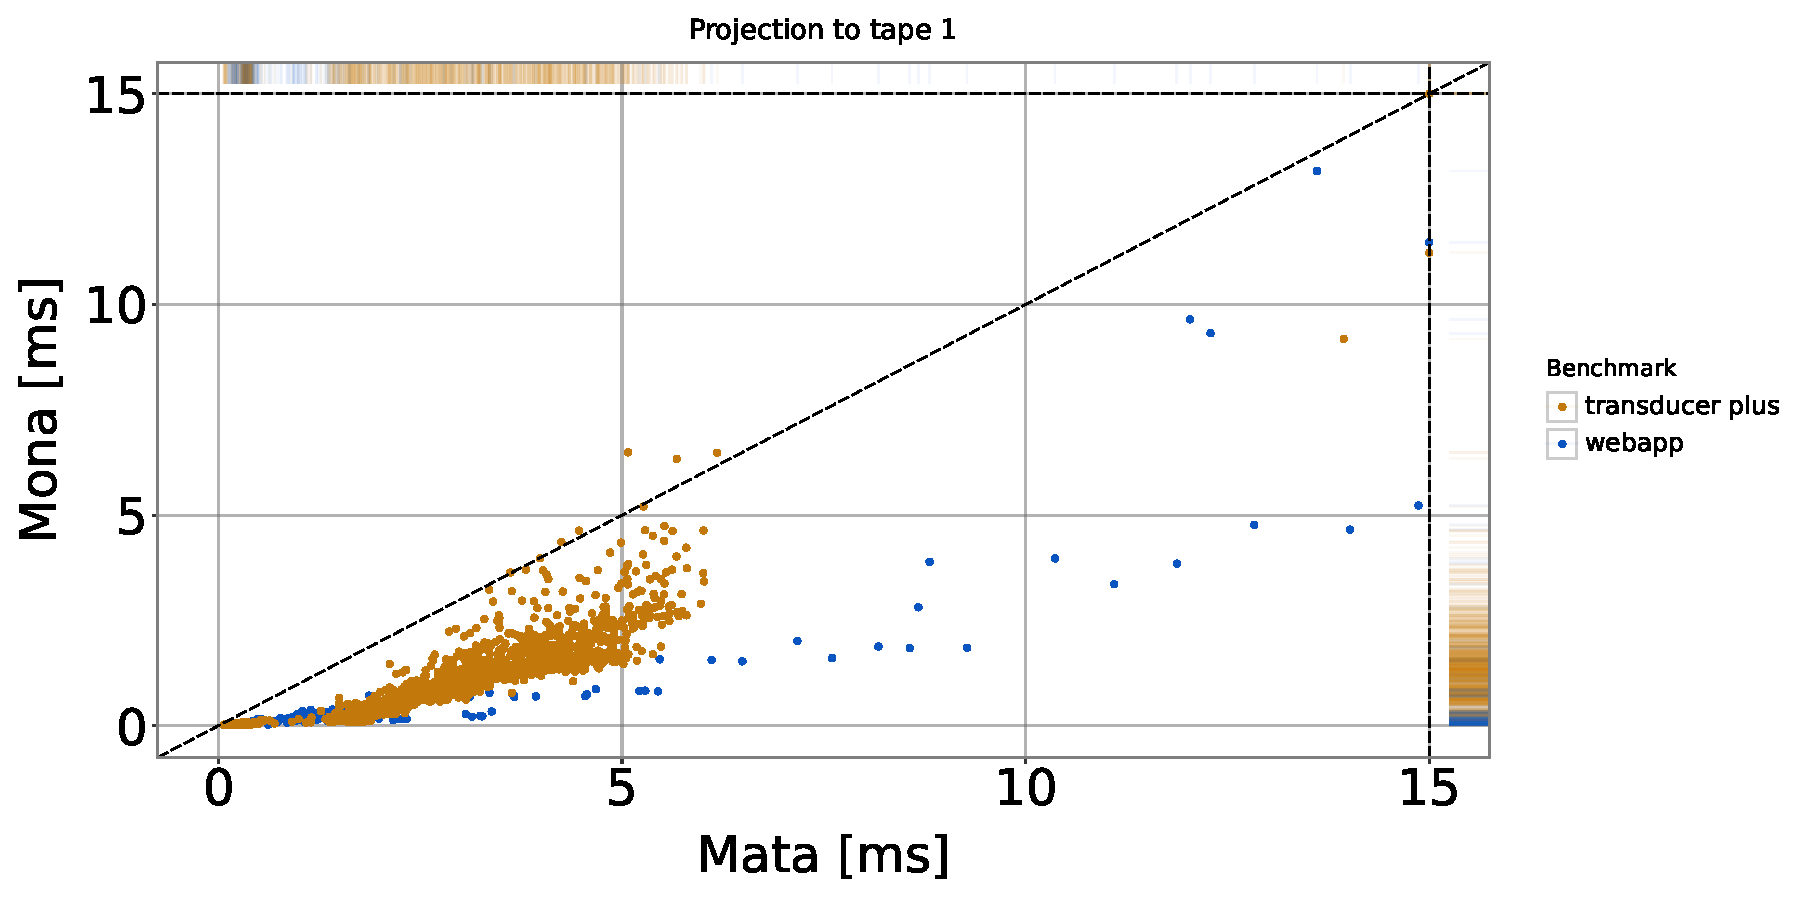
\includegraphics[keepaspectratio, width=0.45\textwidth]{projection_scatter_0.pdf}
    }}%
    \quad
    \subfloat[
      Projection to tape $0$ (projecting out the tape $1$).
      \label{fig:projection_1}
    ]{{
      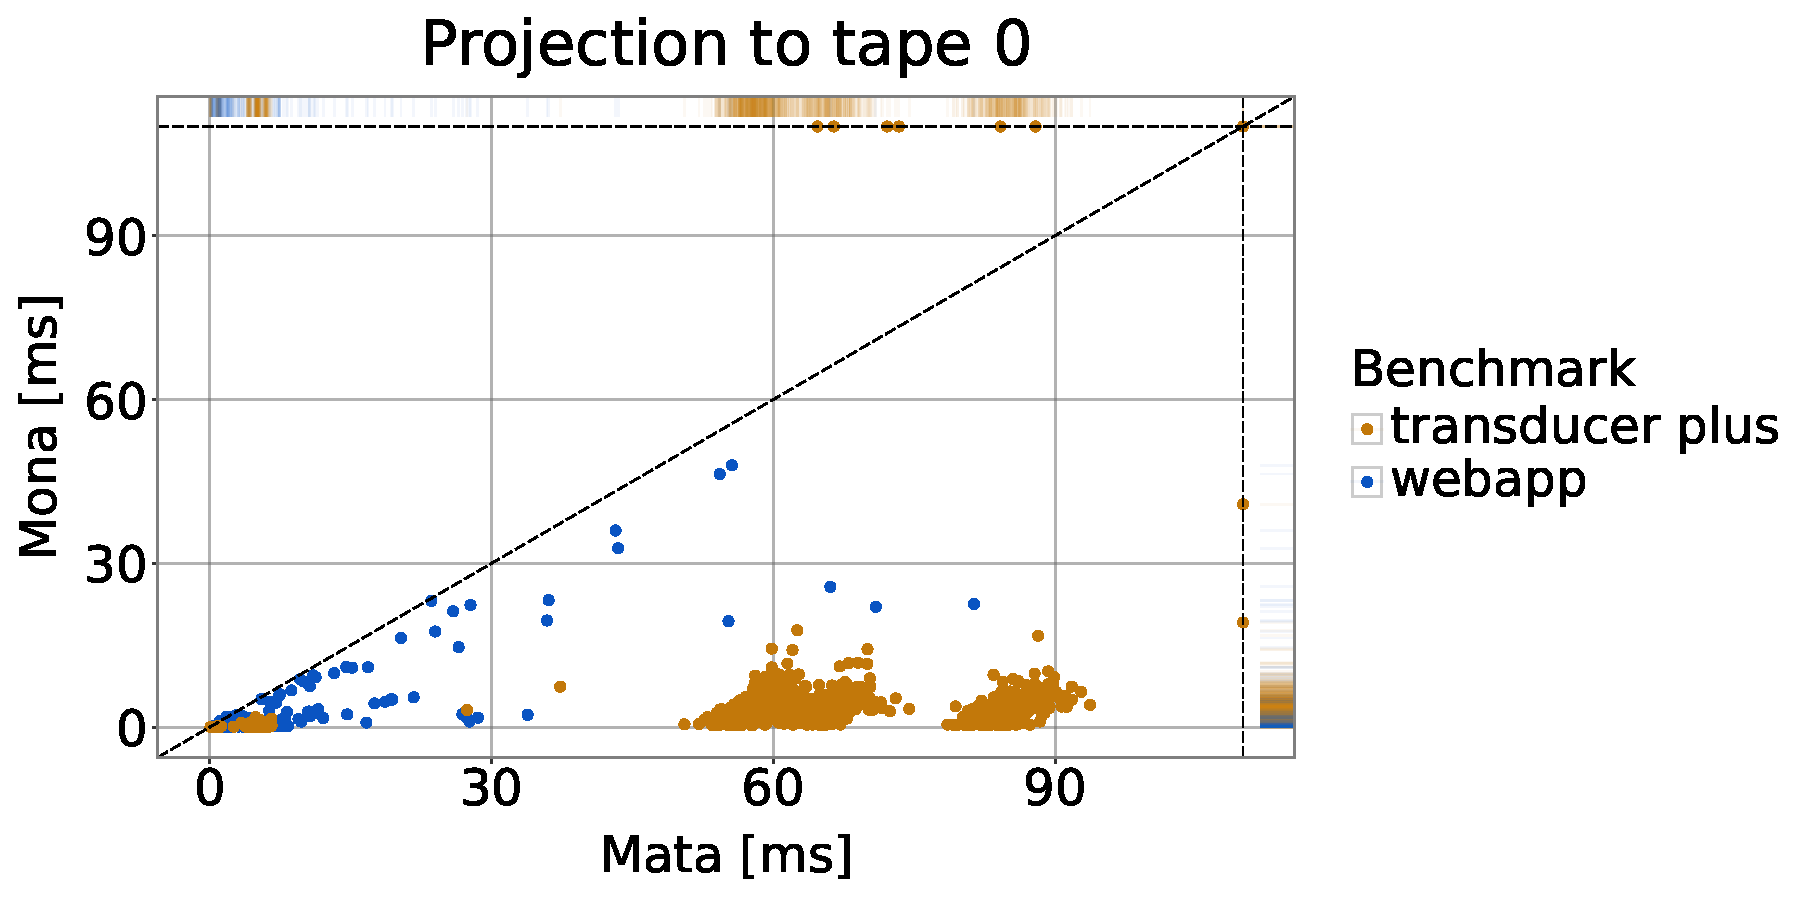
\includegraphics[keepaspectratio, width=0.45\textwidth]{projection_scatter_1.pdf}
    }}%
    \caption{
      Scatter plots comparing performance of \mata and \mona on operation projection.
    }
    \label{fig:projection}%
\end{figure}

We can see that all projections to tape $1$ finish in under $350$ ms in \mata.
By comparing means, we can see that the \mata is about 2 times slower than \mona, but is still fast, finishing $75\%$ of executions in under $4$ ms, compared to \mona's runtime under $3$ ms.

On the other hand, projecting to tape $0$, i.e., projecting out the tape $1$ is more expensive operation for \mata in the implemented data structure.
However, even than \mata finishes $0.75\%$ of executions in under $70$ ms.
Comparing to \mona, encoding of \nfts in \mona ensures that the projecting out the tape $1$ is similarly expensive to projecting out the tape $0$.
If the performance of \mata on projection to tape $0$ proves insufficient when support for \nfts is added in \noodler, one can omit projecting synchronization levels after every composition (and keep the synchronization levels inside the \nft), or apply the suggested specialization for composition for $2$-tape \nfts which does not need to perform projection at all.

\subsection{Application}

On each unique \nft, we applied a word and a language using \nft application.

% \subsubsection{Application of a Language}

Table~\ref{tab:language_application} shows comparison of performance of \mata and \mona on the application operation on both benchmarks applying a language $\Sigma^*$.
The language is forward applied to the \nft ($\idNft{\Sigma^*} \composePipe \ft $).
This simulates the forward image propagation, as described in~\ref{sec:string_solving_with_replace}.

Table~\ref{tab:language_application_backward} shows comparison of performance of \mata and \mona on the application operation on both benchmarks applying a language $\Sigma^*$.
The language is backward applied to the \nft ($\ft \composePipe \idNft{\Sigma^*}$).
This simulates the backward image propagation, as described in~\ref{sec:string_solving_with_replace}.

\begin{table}[ht]
  \centering
  \begin{tabular}{lrrrrrrrr}
\hline
 method   &   TOs &   min &   max &   mean &   q(0.25) &   median &   q(0.75) &   std. dev \\
\hline
 mata     &  1 &  0.12 &  7.59 &   3.72 &      1.37 &     4.47 &      4.92 &       1.87 \\
 mona     &  1 &  0.03 &  0.98 &   0.37 &      0.24 &     0.44 &      0.47 &       0.16 \\
\hline
\end{tabular}

  \caption{
    Language application on both benchmarks where the language is forward applied ($\idNft{\Sigma^*} \composePipe \ft$), simulating the forward image propagation.
  }
  \label{tab:language_application}
\end{table}

\begin{table}[ht]
  \centering
  \begin{tabular}{lrrrrrrrr}
\hline
 method   &   TOs &   min &      max &   mean &   q(0.25) &   median &   q(0.75) &   std. dev \\
\hline
 mata     &  5 &  0.20 & 98138.12 & 436.31 &      5.95 &    31.09 &     50.79 &    4598.41 \\
 mona     &  5 &  0.05 &  8186.49 &  45.42 &      1.18 &    17.19 &     46.31 &     298.65 \\
\hline
\end{tabular}

  \caption{
    Language application on both benchmarks where the language is backward applied on the \nft ($\ft \composePipe \id{\langof{\pi}}$), simulating backward image propagation.
  }
  \label{tab:language_application_backward}
\end{table}

% \subsubsection{Application of a Literal}

Table~\ref{tab:literal_application} shows comparison of performance of \mata and \mona on the application operation on both benchmarks applying a literal.

\begin{table}[ht]
  \centering
  \begin{tabular}{lrrrrrrrr}
\hline
 method   &   TOs &   min &   max &   mean &   q(0.25) &   median &   q(0.75) &   std. dev \\
\hline
 mata     &  0 &  0.14 &  0.69 &   0.24 &      0.22 &     0.24 &      0.26 &       0.05 \\
 mona     &  0 &  0.17 &  0.52 &   0.25 &      0.24 &     0.25 &      0.26 &       0.05 \\
\hline
\end{tabular}

  \caption{
    Literal application on both benchmarks.
  }
  \label{tab:literal_application}
\end{table}

Table~\ref{tab:literal_application_backward} shows comparison of performance of \mata and \mona on the application operation on both benchmarks backward applying a literal to $\ft$.

\begin{table}[ht]
  \centering
  \begin{tabular}{lrrrrrrrr}
\hline
 method   &   TOs &   min &      max &    mean &   q(0.25) &   median &   q(0.75) &   std. dev \\
\hline
 mata     & 17 &  0.16 & 97877.41 & 1041.72 &      4.93 &    26.39 &     48.24 &    8292.23 \\
 mona     &  5 &  0.05 &  8692.85 &   82.55 &      0.86 &    12.67 &     42.16 &     547.51 \\
\hline
\end{tabular}

  \caption{
    Backward literal application on both benchmarks.
  }
  \label{tab:literal_application_backward}
\end{table}

\begin{figure}[ht]
    \centering
    \subfloat[
      Literal application.
      \label{fig:apply_literal}
    ]{{
      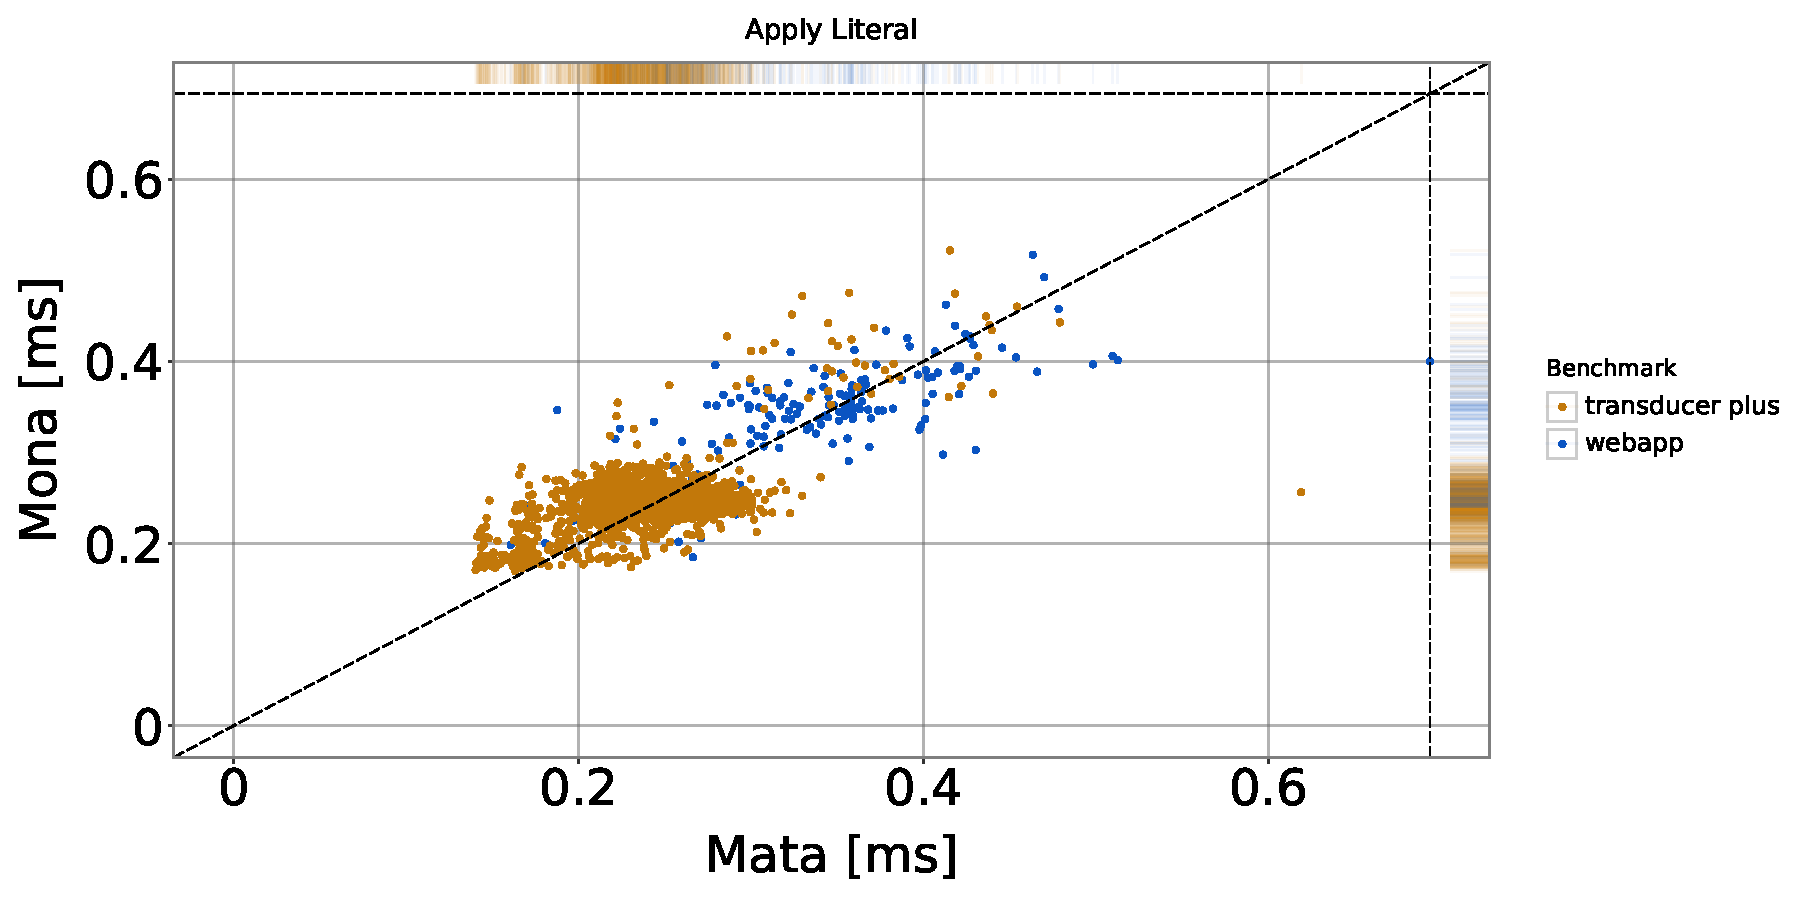
\includegraphics[keepaspectratio, width=0.45\textwidth]{apply_literal_scatter.pdf}
    }}%
    \quad
    \subfloat[
      Language application.
      \label{fig:apply_language}
    ]{{
      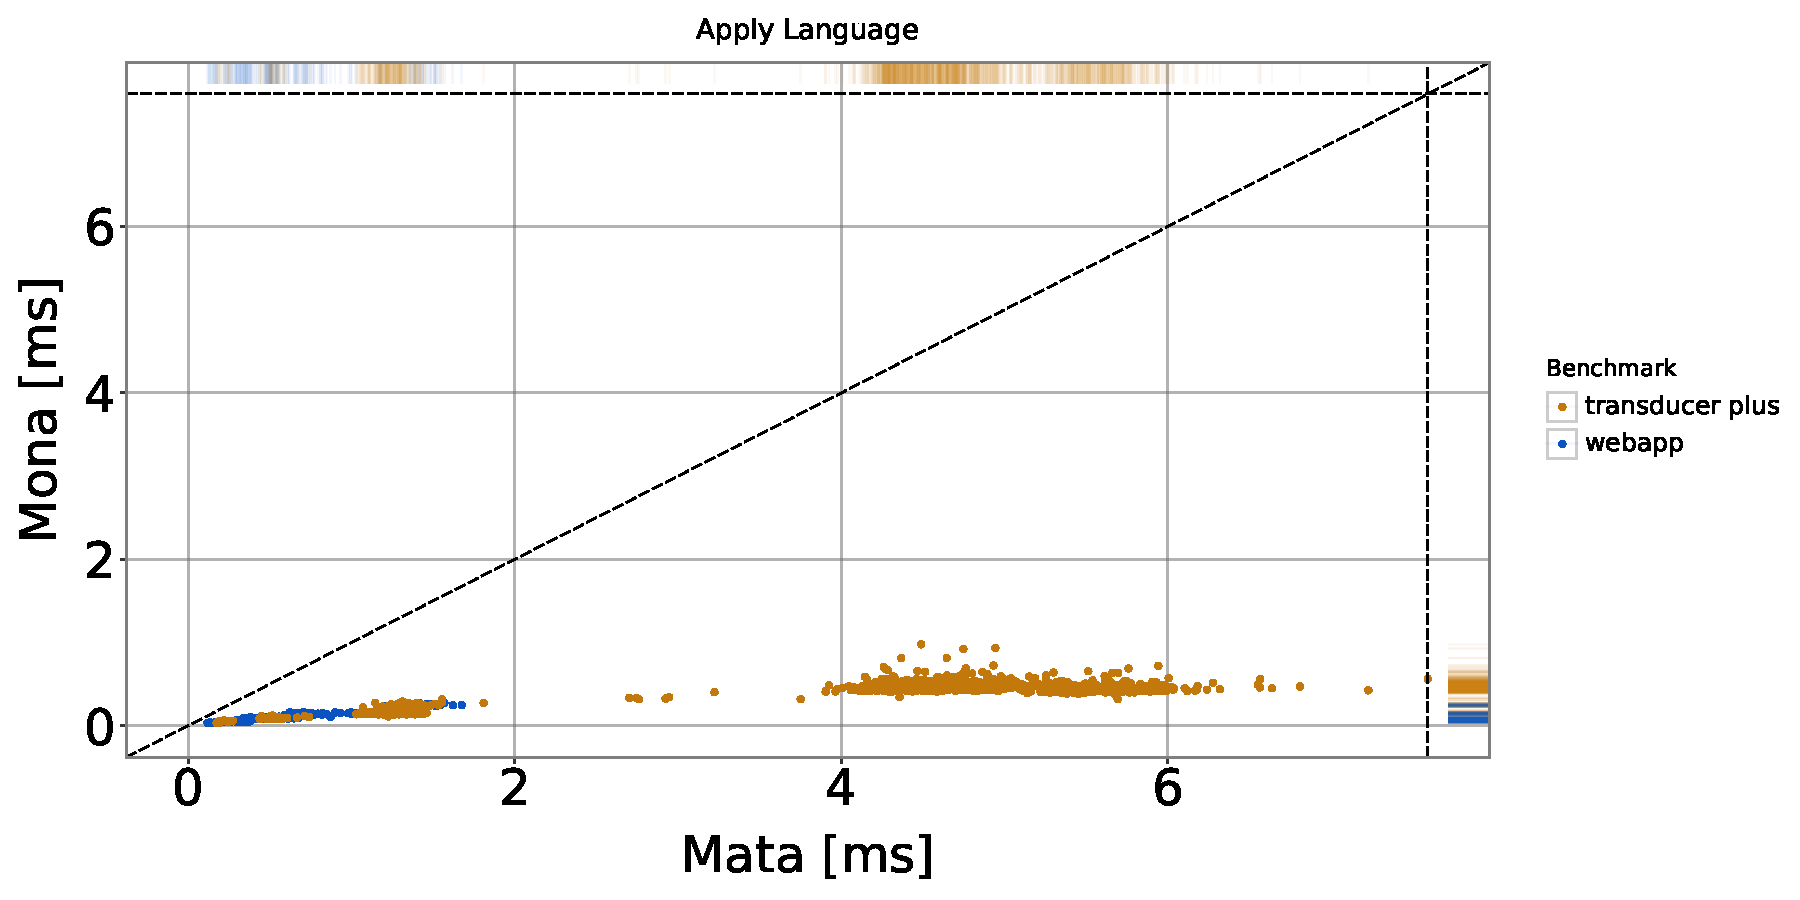
\includegraphics[keepaspectratio, width=0.45\textwidth]{apply_language_scatter.pdf}
    }}%
    \caption{
      Scatter plots for comparing the performance of \mata and \mona on forward application operation on both benchmarks.
    }
    \label{fig:apply_operation}%
\end{figure}

\begin{figure}[ht]
    \centering
    \subfloat[
      Literal application
      \label{fig:apply_literal_backward}
    ]{{
      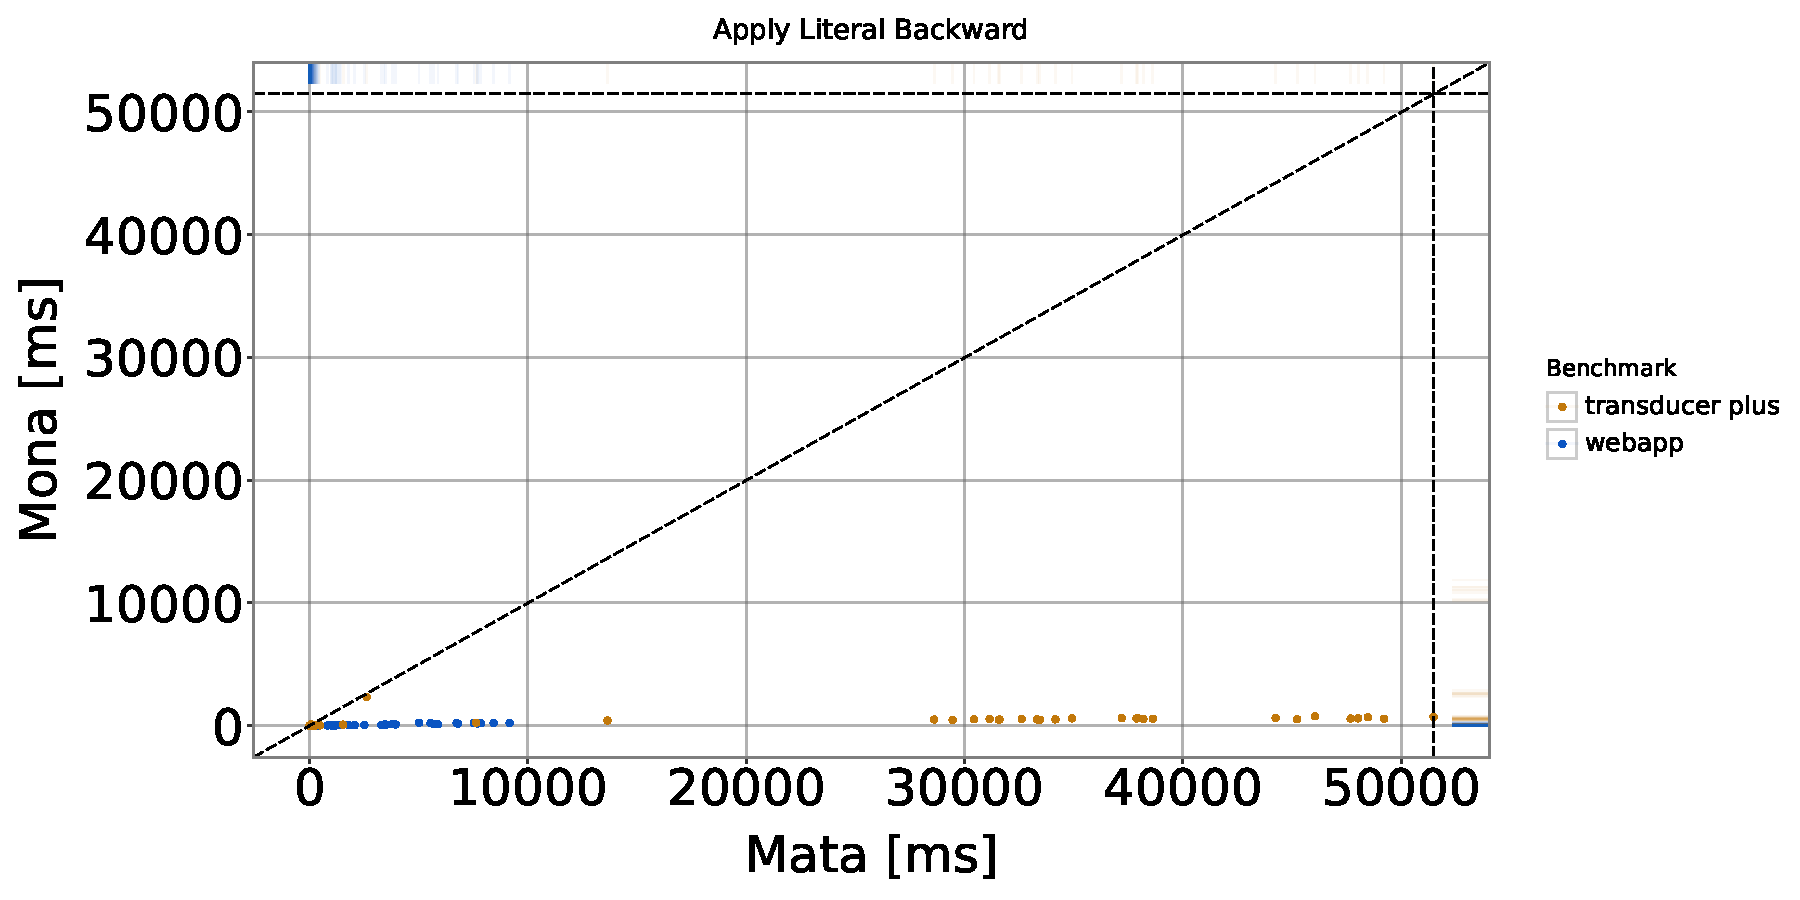
\includegraphics[keepaspectratio, width=0.45\textwidth]{apply_literal_backward_scatter.pdf}
    }}%
    \quad
    \subfloat[
      Language application
      \label{fig:apply_language_bacward}
    ]{{
      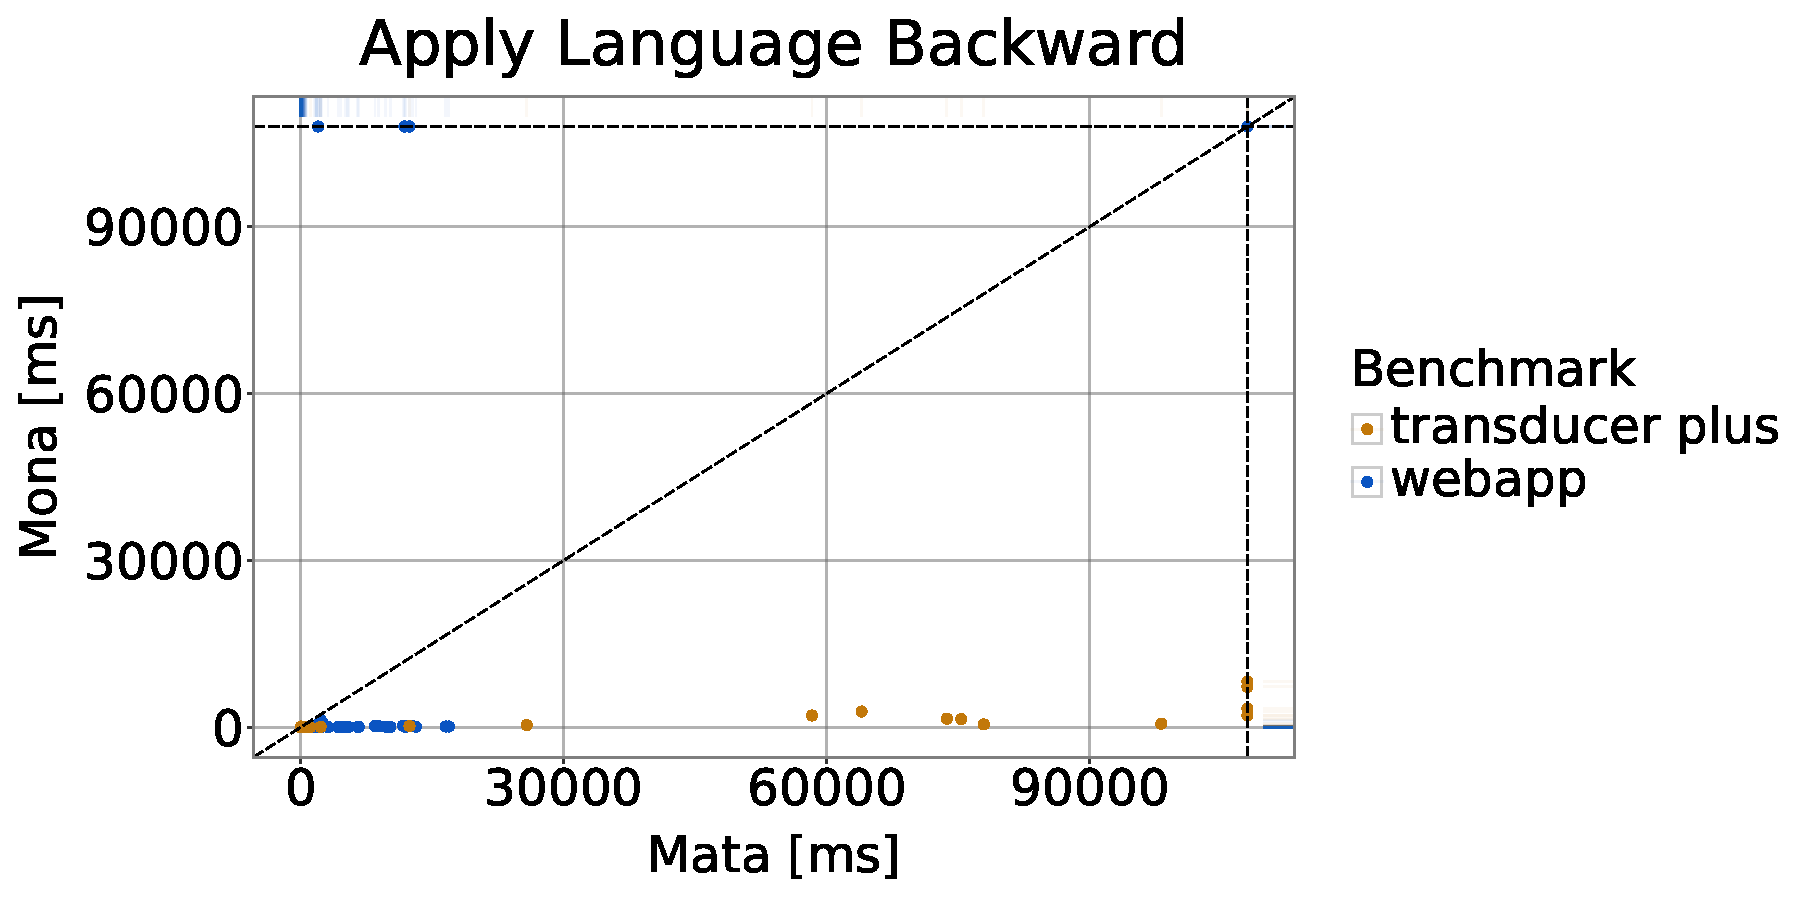
\includegraphics[keepaspectratio, width=0.45\textwidth]{apply_language_backward_scatter.pdf}
    }}%
    \caption{
      Scatter plots for comparing the performance of \mata and \mona on backward application operations on both benchmarks.
    }
    \label{fig:apply_operation_backward}%
\end{figure}

From the results in Table~\ref{tab:literal_application} and Table~\ref{tab:language_application} and scatter plots in Figures~\ref{fig:apply_operation} and~\ref{fig:apply_operation_backward}, we can see that applying a fairly constrainted language (in our case directly a literal) is a quick operation where \mata performs comparably with \mona.
However, applying a large language such as $\Sigma^*$ (used in our experiments), the application gets considerably more expensive for \mata.

This application of $\Sigma^*$ is actually the word case scenario for \mata, as with $\Sigma^*$, \mata must to apply all transition symbols $a \in \Sigma$ for each state $s \in \states$ of $\ft$.
Nevertheless, the computation for both the forward and backward application operations for both the literal and the language finishes in $75\%$ cases in at most $50$ ms, which should be fast enough for \noodler, especially considering the results of the applications and computations can be cached and reused during a run of \noodler.
Notice that for literal application, \mata is about $2$ to $3$ times slower, however, when the language applied gets larger ($\Sigma^*$ in our case), the performance on the 3rd quartile is comparable to \mona on the bacward language application, and only $2$ times slower on the forward language application.

Considering our future uses for application operation in \noodler, we will sometimes apply the whole language $\Sigma^*$, but more often we will apply a more constrained subset $L \subset \Sigma^*$ which should therefore perform better on \noodler runs.
If the performance is then still insufficient, we can implement the aforementioned optimization for composition for $2$-tape \nfts and use in \noodler this version instead of the general application implementation for multi-tape \nfts.

\subsection{Composition}

Table~\ref{tab:composition} shows comparison of performance of \mata and \mona on the composition operation on both benchmarks.

\begin{table}[ht]
  \centering
  \begin{tabular}{lrrrrrrrr}
\hline
 method   &   TOs &   min &      max &   mean &   q(0.25) &   median &   q(0.75) &   std. dev \\
\hline
 mata     & 15 &  0.07 & 54411.24 & 434.64 &      3.20 &     4.16 &     28.52 &    3977.53 \\
 mona     &  0 &  0.05 & 10476.19 &  51.04 &      1.26 &     1.93 &     20.97 &     542.09 \\
\hline
\end{tabular}

  \caption{
    Composition on both benchmarks.
  }
  \label{tab:composition}
\end{table}

Table~\ref{tab:composition_construct_replace} shows comparison of performance of \mata and \mona on the composition operation constructing \nfts for replace operations on both benchmarks.

\begin{table}[ht]
  \centering
  \begin{tabular}{lrrrrrrrr}
\hline
 method   &   TOs &   min &   max &   mean &   q(0.25) &   median &   q(0.75) &   std. dev \\
\hline
 mata     &  0 &  0.15 & 25.52 &   6.35 &      2.48 &     7.89 &      8.89 &       3.49 \\
 mona     &  0 &  0.18 & 25.44 &   2.59 &      1.01 &     2.73 &      3.52 &       1.81 \\
\hline
\end{tabular}

  \caption{
    Composition constructing \nfts for replace operations on both benchmarks.
  }
  \label{tab:composition_construct_replace}
\end{table}

\begin{figure}[ht]
    \centering
    \subfloat[
      Composition operation.
      \label{fig:composition_pair}
    ]{{
      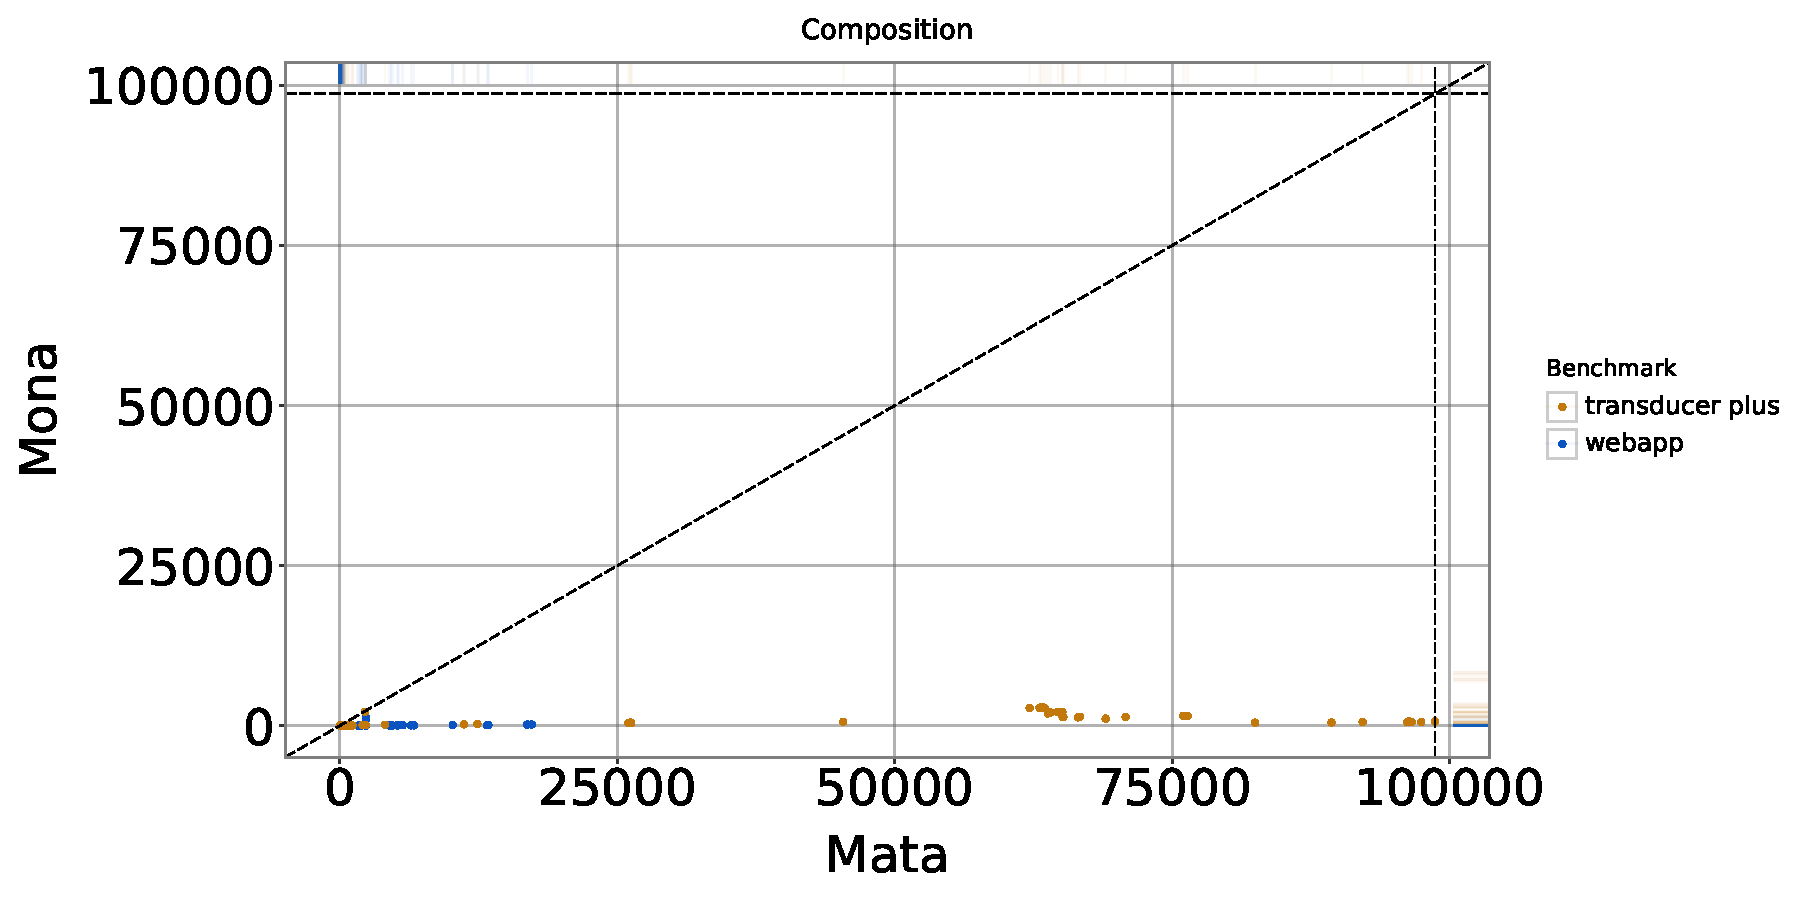
\includegraphics[keepaspectratio, width=0.45\textwidth]{composition_scatter.pdf}
    }}%
    \quad
    \subfloat[
      Composition constructing replace operations.
      \label{fig:composition_construct_replace}
    ]{{
      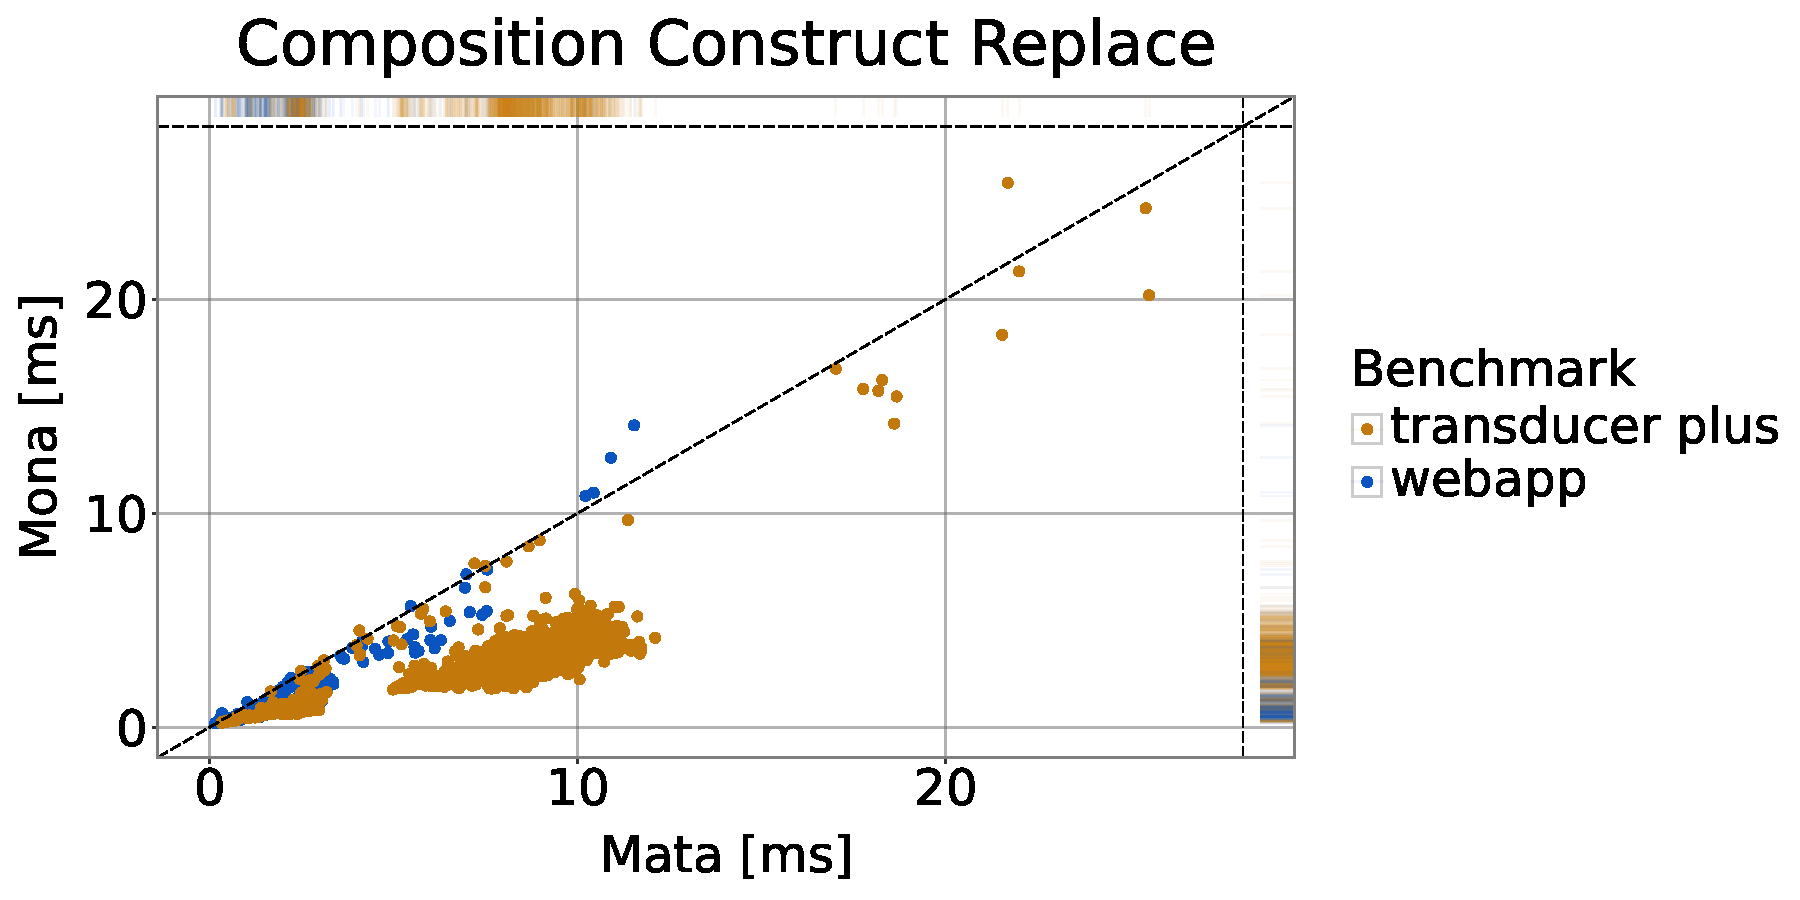
\includegraphics[keepaspectratio, width=0.45\textwidth]{composition_construct_replace_scatter.pdf}
    }}%
    \caption{
      Scatter plots for comparing the performance of \mata and \mona on composition operations on both benchmarks.
    }
    \label{fig:composition}%
\end{figure}

We can see that performance of \mata is comparable to the performance of \mona on a large number of instances for composition constructing replace \nfts, but there is also a similarly large group of instances in the \transducerPlus benchmark where \mata runs slower.
\mata also has 15 timeouts on the largest compositions created as a partial compositions of a long sequence of compositions.

In general, the runtime of \mata is sufficient.
We can see that $75 \%$ of instances common in string solving are solved in less than $28$ ms in \mata compared to $21$ ms in \mona.
Only the partial compositions containing considerably larger \nfts show noticeable slowdown for \mata.

As mentioned earlier, if the performance of \nfts in \mata proves to be a bottleneck in string solving, a specialized algorithm for composition of $2$-tape \nfts can be used instead of the general algorithm for multi-tape \nfts.

\subsection{Pattern matching benchmark.}

The Table~\ref{tab:symbol_from_end_apply_language} shows the comparison of \mata and \mona on pattern matching benchmark \symbolFromEnd on language application operation.

\begin{table}[ht]
  \centering
  \begin{tabular}{lrrrrrrrr}
\hline
 method   &    TOs &   min &      max &    mean &   q(0.25) &   median &   q(0.75) &   std. dev \\
\hline
 mata     &   0 &  0.97 &  8070.18 & 2397.81 &    461.98 &  1743.10 &   4035.48 &    2233.84 \\
 mona     & 272 &  0.29 & 13095.06 & 1614.42 &      2.39 &    39.25 &    970.33 &    3485.11 \\
\hline
\end{tabular}

  \caption{
    Language application on \symbolFromEnd.
  }
  \label{tab:symbol_from_end_apply_language}
\end{table}

The Table~\ref{tab:symbol_from_end_construct_replace} shows the comparison of \mata and \mona on pattern matching benchmark \symbolFromEnd on the construction of the replace \nft operation.

\begin{table}[ht]
  \centering
  \begin{tabular}{lrrrrrrrr}
\hline
 method   &    TOs &   min &      max &    mean &   q(0.25) &   median &   q(0.75) &   std. dev \\
\hline
 mata     &   0 &  1.79 &  7900.85 & 2211.33 &    446.27 &  1623.44 &   3680.46 &    1983.68 \\
 mona     & 232 &  1.04 & 12664.70 & 2987.85 &     79.46 &  1304.86 &   4614.69 &    3791.32 \\
\hline
\end{tabular}

  \caption{
    Composition for replace construction on \symbolFromEnd.
  }
  \label{tab:symbol_from_end_construct_replace}
\end{table}

\begin{figure}[ht]
    \centering
    \subfloat[
      Language application.
      \label{fig:symbol_from_end_apply_language}
    ]{{
      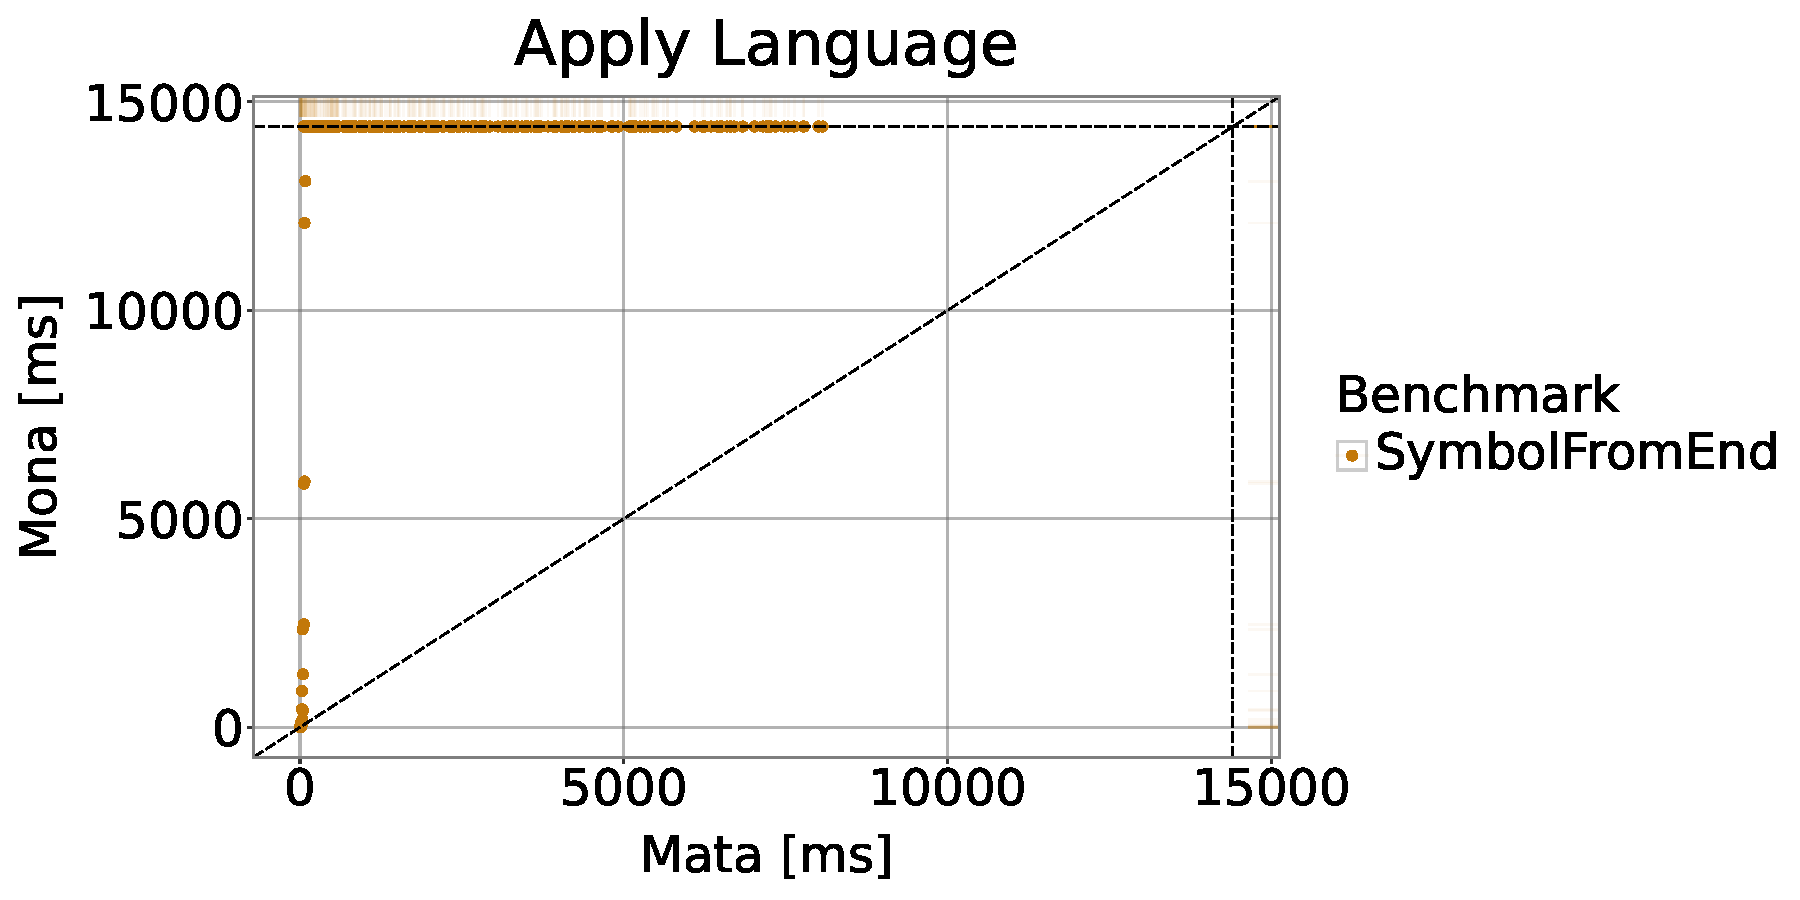
\includegraphics[keepaspectratio, width=0.45\textwidth]{symbol_from_end_apply_language_scatter.pdf}
    }}%
    \quad
    \subfloat[
      Composition constructing replace operations.
      \label{fig:symbol_from_end_composition_construct_replace}
    ]{{
      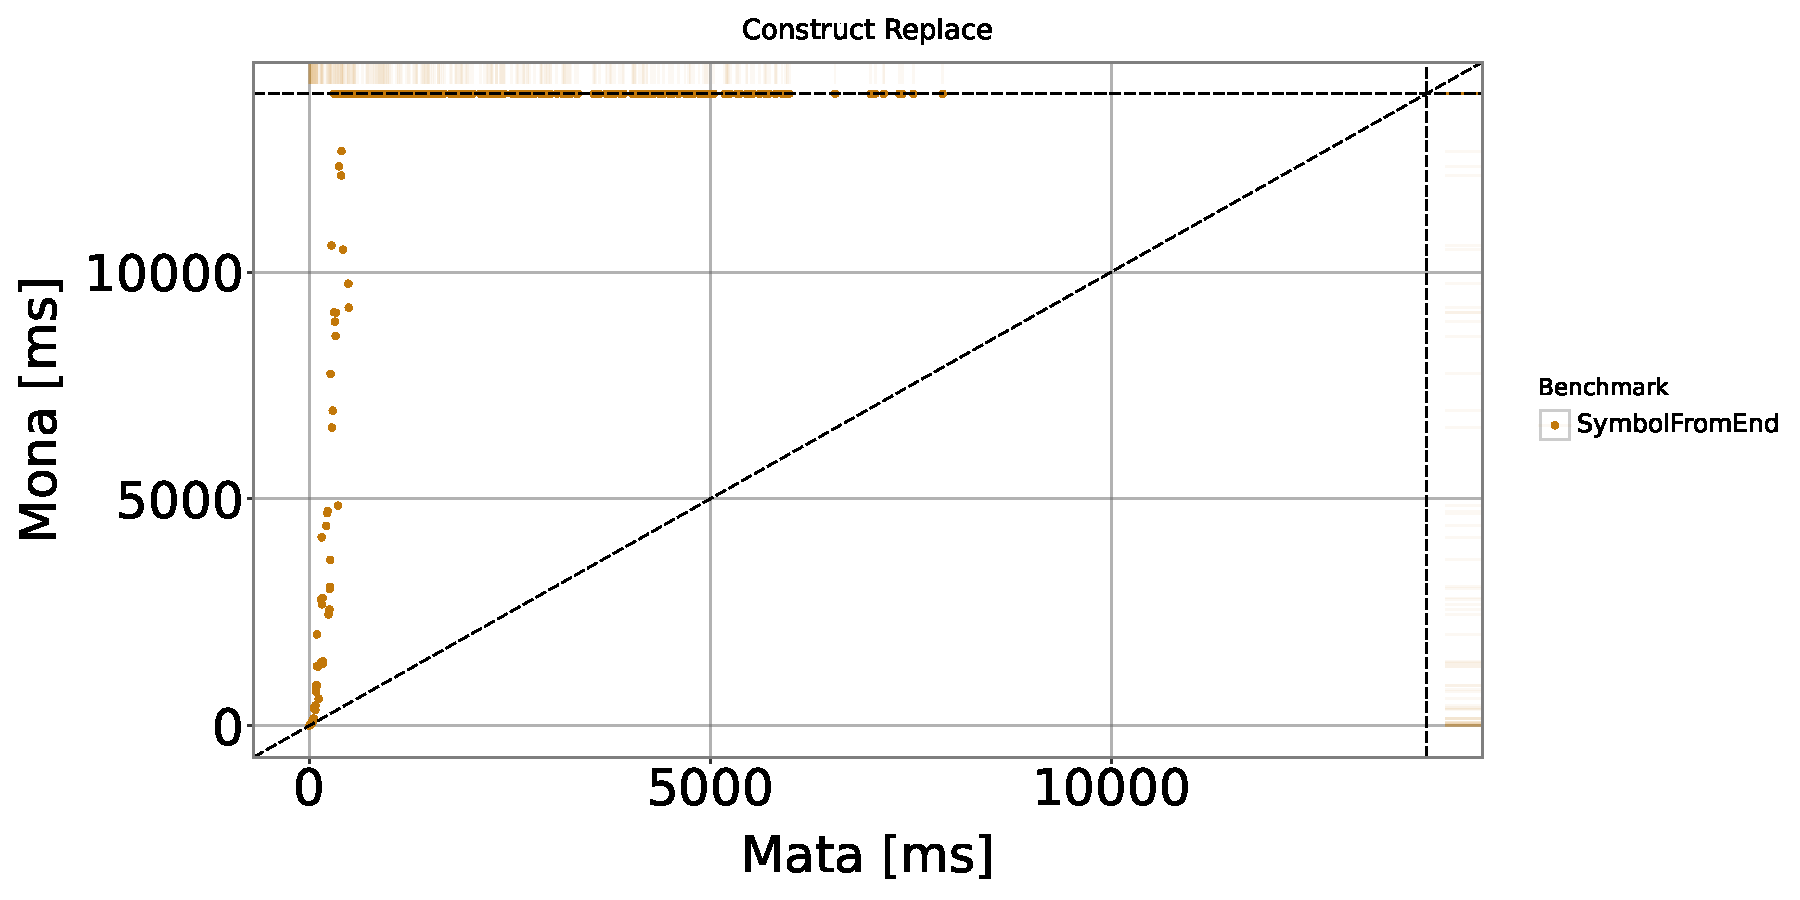
\includegraphics[keepaspectratio, width=0.45\textwidth]{symbol_from_end_construct_replace_scatter.pdf}
    }}%
    \caption{
      Scatter plots for comparing the performance of \mata and \mona on \symbolFromEnd.
    }
    \label{fig:symbol_from_end}%
\end{figure}

\mata computed all pattern matching benchmarks quickly, running at most $8$ s on the largest instance with $150$ repetitions on the language application operation.
\mona managed to compute only the first smallest $14$ instances (for both the replace single and replace all variants, in total finishing $28$ on instances).
In the remaining $272$ instances, \mona fails to determinize the pattern and runs out of memory.

The similar results can be seen in construction of replace \nfts. Even if the intermediate \nfts are small compared to the final \nfts for replace operations, \mona manages to compute only the first smallest $35$ instances (for both the replace single and replace all variants, in total finishing on $70$ instances).
In the remaining $232$ instances, \mona fails to determinize the pattern and runs out of memory.

This benchmark clearly shows that once you start using \nfts on problems from practice more complex than the simple replace operations in string solving benchmarks from SMT-LIB, the ability to use explicit symbols on transitions and handling nondeterminism becomes crutial to all tools applicable to these problem domains.

\section{Summary}

The experiments show that \mata has higher base runtime in comparision with \mona, but in general, $75 \%$ of examples are finished in about the same time in \mata as in \mona, finishing in under $50$ ms.
\mata runs comparably with \mona on application of a literal and projection to tape $1$.
Otherwise, \mata runs slower than \mona, but even then its runtime is reasonable.
There are a few instances where \mata fails to compute the composition and times out whereas \mona succeeds in computing the composition.

Considering that \mona is a well-optimized library for applications on binary representations of transition symbols, we consider a success that \nfts in \mata are able to get close to the performance of \mona, and even outperform \mona in some cases.

For most cases, the performance of \mata should be improved by implementing the optimized composition specialized for $2$-tape \nfts which omits having to insert self-loops and additional levels into the composed \nfts.

The experiments shown are not the only use cases for \nfts in \mata, but they represent a selection of operations that will be performed in \noodler.
Furthermore, the instances of replace operations appearing in SMT-LIB benchmarks are relatively small and easy to compute.
When applying \nfts to examples from practice from other domains, e.g., pattern matching~\cite{10.1007/978-3-031-30829-1_19}, the patterns being matched get progressively larger and introduce more nondeterminism.
With the larger patterns, the advantage of \mata being able to handle nondeterminism naturally should prove to be crutial for efficient creation and handling the corresponding \nfts, quickly outperforming tools without proper support for nondeterminism.
That is because the complexity of determinization of similar patterns usually increases exponentially to the number in counters.

We conclude that \nfts in \mata are prepared and ready to be used in \noodler and the experimental evaluation shows that the performance of \mata should be sufficient for the uses in string solving.
Moreover, we conclude that \nfts in \mata are capable of handling complex tasks such as working with regular expressions with counting operations and are generally applicable to a large group of domains beside string solving.

\chapter{Conclusion}

To summarize this thesis, we have added support for a new model for finite state machines, finite state transducers, to \mata, explained the principles behind \nfts and specifically \nfts in the context of \mata and \noodler for string solving.

We have created a new data structures derived from the existing data structures for \nfas in \mata, which fit well in the overall structure and design decision of \mata.
The introduced algorithms on \nfts are closely related to the corresponding algorithms on BDDs and maintain the two main goals of \mata: simplicity and efficiency, while keeping \mata easily extensible and understandable for a wide variety of users and applicable to both the areas of automata research and industry.

Thanks to these design decision, further extending \mata with support for handling BDDs will be effortless.

We further focussed on utilizing \nfts in string solving by adding algorithms to model string replace operations defined in SMT-LIB which will be used in \noodler for solving SMT formulae with string replace operations, previously unsolvable by \noodler.

We compared the performance of \nfts in \mata with a natural encoding of transducers in the automata library \mona.

The experiments show that \mata performs slower than \mona in string solving, but still runs reasonably fast.
When applied on complex regular expressions such as pattern matching, \mata clearly outperforms approaches without proper handling for explicit alphabets with nondeterminism.
The performance of \mata on $2$-tape \nfts can be further improved by applying the specialized algorithm for composition for $2$-tape \nfts, or by sometimes preventing execution of projection.

Overall, the design and implementation of \nfts in \mata is feasible, functional, performs sufficiently enough, and is widely usable, with ready-for-use support for solving SMT formulae with string replace operations in \noodler.

\paragraph{Future work.}
We continue optimizing and developing \mata and the implementation of \nfts.
In the future, we want to apply \nfts to solving string SMT formulae in \noodler.
Furthermore, depending on the performance of \nfts in \noodler, we intend to add support for symbolic representations for large alphabets using bit vectors representing sequences of bits, as used in tool \lash~cite{lash} and transition representation specific to \nfts to encode \nft operations such as identity more easily.

If the performance of composition of \nfts in \noodler proves to be a bottleneck, we can implement the optimized algorithm specialized for $2$-tape \nfts.

Since the representation of \nfts in \mata is close to BDDs, we intend to study various optimizations used for BDDs to further improve the performance of \nfts in \mata.

Finally, we intend to inherit the current structure for \nfts with the corresponding operations and add support for BDDs to \mata for future uses.


%=========================================================================

% For compilation piecewise (see projekt.tex), it is necessary to uncomment it
% \end{document}
